% Suggested LaTeX style template for Masters project report submitted at the
% Department of Computer Science and Technology
%
% Markus Kuhn, May 2022
% (borrowing elements from an earlier template by Steven Hand)

\documentclass[12pt,a4paper,twoside]{report}
% append option ",openright" after "twoside" if you prefer each chapter
% to start on a recto (odd-numbered) page in a double-sided printout

\usepackage[pdfborder={0 0 0}]{hyperref}  % turns references into hyperlinks
\usepackage[vmargin=20mm,hmargin=25mm]{geometry}  % adjust page margins
\usepackage{graphicx} % allows inclusion of PDF, PNG and JPG images
\usepackage{subcaption}
\usepackage{parskip}  % separate paragraphs with vertical space
                      % instead of indenting their first line
\usepackage{setspace} % for \onehalfspacing
\usepackage{refcount} % for counting pages
\usepackage{upquote}  % for correct quotation marks in verbatim text

\usepackage{amsmath}
\usepackage{amssymb}
\usepackage{float}
\usepackage{svg}
\usepackage[numbers,sort&compress]{natbib}
\usepackage{tcolorbox}

\usepackage{algorithm}
\usepackage{algpseudocode}

\newif\ifsubmission % Boolean flag for distinguishing submitted/final version

% Change the following lines to your own project title, name, college, course
\title{\protect\textsc{Carico}: Scheduling via Federated Workload Capacity Estimation}
\author{Luca Choteborsky}
\date{June 2025}
\newcommand{\candidatenumber}{1234N}
\newcommand{\college}{Selwyn College}
\newcommand{\coursethe}{Computer Science Tripos, Part III}
\newcommand{\coursefor}{Part III of the Computer Science Tripos}

% Select which version this is:
% For the (anonymous) submission (without your name or acknowledgements)
% uncomment the following line (or let the makefile do this for you)
%\submissiontrue
% For the final version (with your name) leave the above commented.

\begin{document}
\pagenumbering{roman}

\begin{sffamily} % use a sans-serif font for the pro-forma cover sheet

\begin{titlepage}
\makeatletter

% University logo with shield hanging in left margin
\hspace*{-14mm}
\includegraphics[width=65mm]{logo-dcst-colour}

\ifsubmission

% submission proforma cover page for blind marking
\begin{Large}
\vspace{20mm}
Research project report title page

\vspace{35mm}
Candidate \candidatenumber

\vspace{42mm}
\textsl{``\@title''}

\end{Large}

\else

% regular cover page
\begin{center}
\Huge
\vspace{\fill}

\@title
\vspace{\fill}

\@author
\vspace{10mm}

\Large
\college
\vspace{\fill}

\@date
\vspace{\fill}

\end{center}

\fi

\vspace{\fill}
\begin{center}
Submitted in partial fulfillment of the requirements for the\\
\coursethe
\end{center}

\makeatother
\end{titlepage}

\newpage

Total page count: \pageref{lastpage}

% calculate number of pages from
% \label{firstcontentpage} to \label{lastcontentpage} inclusive
\makeatletter
\@tempcnta=\getpagerefnumber{lastcontentpage}\relax%
\advance\@tempcnta by -\getpagerefnumber{firstcontentpage}%
\advance\@tempcnta by 1%
\xdef\contentpages{\the\@tempcnta}%
\makeatother

Main chapters (excluding front-matter, references and appendix):
\contentpages~pages
(pp~\pageref{firstcontentpage}--\pageref{lastcontentpage})

Main chapters word count: 467

Methodology used to generate that word count:

[For example:

\begin{quote}
\begin{verbatim}
$ make wordcount
gs -q -dSAFER -sDEVICE=txtwrite -o - \
   -dFirstPage=6 -dLastPage=11 report-submission.pdf | \
egrep '[A-Za-z]{3}' | wc -w
467
\end{verbatim}
\end{quote}

]

\end{sffamily}

\vspace{\fill}
\onehalfspacing
\textbf{\Huge Declaration}
\vspace{40pt}

I,
\makeatletter\ifsubmission
\candidatenumber,
\else
\@author\ of \college,
\fi\makeatother
being a candidate for \coursefor, hereby declare that this report and
the work described in it are my own work, unaided except as may be
specified below, and that the report does not contain material that
has already been used to any substantial extent for a comparable
purpose.
In preparation of this report, I adhered to the
\href{https://www.cst.cam.ac.uk/files/ai_policy.pdf}{Department of
Computer Science and Technology AI Policy}. I am content for
my report to be made available to the students and staff of the
University.

% Remove the [...] sentence or just the brackets, as appropriate.
% Substitute the {insert name of technology} text above as required.

% Add here things like: Figure X is the work of Y, etc.

\ifsubmission\else
\bigskip
\textbf{Signed:}
\fi

\bigskip
\textbf{Date:}
\vspace{\fill}

\chapter*{Abstract}

Kubernetes is an existing widely-used open-source container orchestration system
that automates the deployment, scaling and management of containerized
applications. Efficient scheduling is a critical component of Kubernetes,
dictating an optimal allocation of pods across nodes to maximise a set of goals.
Kubernetes schedulers generally fall into two categories: pod-descriptive and
telemetric-based. Pod-descriptive schedulers, like the default
\texttt{kube-scheduler}, rely on accurately defined Pod resource requests for
optimal performance. In contrast, telemetric-based schedulers leverage collected
Node metrics to identify under or over-utilized Nodes. While these are often
used to refine decisions made by existing pod-descriptive schedulers, this
dissertation focuses on exploring the potential of a telemetric-only scheduler.

Scheduling in Kubernetes without explicit Pod resource requests remains largely
unexplored due to its complexity. Traditional bin-packing approaches are
insufficient; instead, a telemetric-only scheduler requires a novel strategy to
derive optimal plans from collected telemetry.

PRONTO offers a promising direction. This federated, asynchronous, and
memory-limited algorithm schedules tasks across hundreds of workers. It enables
individual workers to build local workload models from telemetry, which are then
aggregated to form a global system view. For a telemetric-only scheduler,
maximizing information aggregation is crucial. However, in very large clusters,
centralizing all this data quickly becomes a bottleneck. By distributing the
knowledge federation workload across the cluster, we can significantly reduce
the load on a central scheduler.

Unfortunately, PRONTO's direct application to Kubernetes proved unfeasible due
to its communication latency assumptions and early empirical findings.
Consequently, I propose CARICO (Italian for "load"), a novel scheduler that
shares PRONTO's core properties but accounts for communication latency. CARICO
enables Nodes to perform FSVD on capacity-based metrics, modeling past resource
usage to estimate future workload capacity.

To evaluate CARICO, I implemented a prototype within the Kubernetes ecosystem.
This involved extensive investigation into various metrics and filters to
generate a precise capacity signal. Finally, I benchmarked CARICO's overall
performance against the default kube-scheduler on a Kubernetes cluster with
diverse workloads. While CARICO achieved comparable throughput, it significantly
outperformed kube-scheduler as a QoS scheduler, demonstrating lower Pod
Completion times and improved workload isolation.

\ifsubmission\else
% not included in submission for blind marking:

\chapter*{Acknowledgements}

I would like to thank both my supervisors, Andreas Grammenos and Eva
Kalyvianaki, for their guidance and assistance during this project and their
work with \textsc{Pronto}, the foundation on top of which this dissertation is
based. I would also like to thank my Director of Studies, Richard Watts, for his
support throughout my academic studies.

\fi
\cleardoublepage % preserve page numbers after missing acknowledgements

\tableofcontents
\listoffigures
%\listoftables

\chapter{Introduction (961)}
\label{firstcontentpage} % start page count here

% This is the introduction where you should introduce your work. In
% general the thing to aim for here is to describe a little bit of the
% context for your work -- why did you do it (motivation), what was the
% hoped-for outcome (aims) -- as well as trying to give a brief overview
% of what you actually did.
%
% It's often useful to bring forward some ``highlights'' into this
% chapter (e.g.\ some particularly compelling results, or a particularly
% interesting finding).
%
% It's also traditional to give an outline of the rest of the document,
% although without care this can appear formulaic and tedious. Your
% call.

% Kubernetes is a widely-used open-source container orchestration system that
% automates the deployment, scaling and management of containerized applications.
% It can run production workloads, having becoming the foundation for many cloud
% computing services like Google Cloud and AWS, while also being portable and
% extensible with a rapidly growing ecosystem of support and tools. Efficient
% scheduling is a critical component of Kubernetes, dictating how deployments
% are best allocated across nodes and ensuring no individual node is overloaded.
% Existing Kubernetes schedulers can be classified according to the input data
% they use to inform scheduling decisions: pod-description vs. telemetry. The
% performance of pod-description based schedulers relies on accurate workload
% estimations which is not always available. Meanwhile, telemetry-based schedulers
% use live information to maximise resource utilisation of nodes and prevent them
% from becoming overloaded. These telemetry-based schedulers typically use
% utilisation metrics which can be overly sensitive and generate false
% notifications of full capacity.
%

Kubernetes has firmly established itself as the leading platform for container
orchestration, experiencing widespread adoption across diverse industries and
organizations of all scales~\cite{kubernetes-adoption-statistics}. From
stateless microservices to complex stateful databases, Kubernetes serves as the
infrastructure backbone for cloud computing services like Google
Cloud~\cite{google-gke} and Azure~\cite{azure-aks}. Its versatility, from
supporting machine learning (ML) deployments~\cite{kubernetes-ai}, edge
computing~\cite{cloudraft} end serverless functions~\cite{knative, openwhisk},
solidifies Kubernetes' position as a cornerstone of the cloud-native industry.

A core function of container orchestration is the efficient scheduling of
containers across a cluster. Kubernetes performs online scheduling, a
particularly challenging subset of the NP-hard task-scheduling problem. In
online scheduling, tasks must be allocated without prior knowledge of future
arrivals~\cite{pruhs2004online}. In this dynamic and resource-intensive
landscape, efficient online scheduling is paramount for both performance and
cost-effectiveness. Poor scheduling decisions can lead to significant
infrastructure waste, directly impacting an organization's bottom line.
Misconfiguration in resource requests and limits is a primary cause of
under-utilised resources or idle nodes, leading to higher billing
\cite{cost-strategies,
bin-packing-and-cost-savings-in-kubernetes-clusters-on-aws}.

Kubernetes was built upon the ideas from Borg~\cite{}, a large-scale cluster
management developed and used by Google. Consequently, Kubernetes' default
scheduler~\cite{kube-scheduler} (\texttt{kube-scheduler}) performs bin-packing
based on the resource requests included in Pod descriptions and heuristic-based
capacities calculated from the Nodes' advertised hardware. The performance
achieved by \texttt{kube-scheduler} therefore depends on accurate estimates of
Pod resource usage. While telemetry-based systems have been proposed to improve
scheduling decisions, they often use expensive deep-ML techniques
\cite{bao2019deep, peng2021dl2} or focuses on a per-Node
level~\cite{yang2019design}. These telemetry-based systems typically augment
existing resource requests or re-schedule already running workloads to less
congested Nodes.

\textsc{Pronto} \cite{grammenos_pronto_2021} offers a promising direction for a
purely telemetry-driven approach. This novel federated, asynchronous, and
memory-limited algorithm allows each compute node to work with a
global view of the system by distributing the knowledge federation workload to
reduce the burden on a central scheduler. However, its direct application within
a Kubernetes scheduling
environment faces significant challenges. \textsc{Pronto}'s original design
assumes zero communication latency and yields only a binary "Reject-Job" signal,
which lacks the granularity for sophisticated Node scoring and fails to account
for significant Pod startup latencies observed in real-world Kubernetes clusters
\cite{qadeer_scaling_2022}. Furthermore, empirical investigations into Linux
Pressure Stall Information (PSI) metrics, a potential replacement for the VMware
vSphere CPU-Ready metric, revealed frequent transient spikes attributed to the
container runtime. This would make it difficult to efficiently distinguish
genuine resource contention from noise when collecting a small set of metrics.
These limitations necessitate a more sophisticated signal that is both
\textbf{comparable} for effective Node ranking and \textbf{reservable} to track
the pending impact of in-flight Pods.

\section{Dissertation Aims and Contributions}

This dissertation aims to apply the theory behind \textsc{Pronto} within the
Kubernetes ecosystem by proposing, implementing, and evaluating \textsc{CARICO} (Italian
for "load"), a novel, purely telemetry-driven scheduling algorithm that
maintains the federated, asynchronous, and memory-limited properties of
\textsc{Pronto} explicitly accounting for communication latency.

The key contributions of this project are:
\begin{itemize}
    \item \textbf{Feasibility Analysis of \textsc{Pronto} for Kubernetes:} An
        investigation into the applicability of \textsc{Pronto}'s principles to
        Kubernetes scheduling, highlighting its flawed assumptions and
        presenting empirical evidence for the challenges of using raw telemetry
        metrics.
    \item \textbf{Proposal of \textsc{CARICO}:} A novel federated, asynchronous,
        and memory-limited scoring algorithm that explicitly accounts for
        communication latency.
    \begin{itemize}
        \item Novel application of Federated Singular Value Decomposition (FSVD)
            to build a local model of recent resource usage, adapting the
            standard SVD subspace merge operation for a lack of mean-centering.
        \item Presentation of a novel \textbf{comparable} capacity signal that scores a Node's
            predicted ability to accept new workloads, considering recent
            resource utilisation across the cluster.
        \item Application of simple signal processing techniques to transform
            the generated capacity signal into a \textbf{reservable} metric,
            enabling schedulers to account for communication latencies.
    \end{itemize}
    \item \textbf{Prototype Implementation and Evaluation of \textsc{CARICO}:}
    \begin{itemize}
        \item Extensive investigation into different telemetry metrics and
            signal processing techniques within the setting of a Kubernetes
            cluster to generate an accurate and precise capacity signal.
        \item Analysis of the correctness of the generated signal and
            exploration of approaches for estimating reservation quantities.
        \item Comprehensive evaluation of \textsc{CARICO}'s overall performance
            under various workloads on a real-world Kubernetes cluster,
            comparing its throughput, Quality of Service (QoS), and performance
            isolation against the industry-standard \texttt{kube-scheduler}.
    \end{itemize}
\end{itemize}

\section{Dissertation Overview}
The remainder of this dissertation is structured as follows:
\begin{itemize}
    \item \textbf{Chapter 2 (Background):} This chapter provides foundational
        knowledge, detailing Kubernetes architecture and its scheduling
        mechanism. It introduces \textsc{Pronto}, explaining its core
        mathematics and highlighting its accuracy in predicting performance
        degradation, while also critically examining its weaknesses that
        necessitate a more sophisticated signal. Finally, it reviews existing
        Kubernetes schedulers to contextualize this work within the current
        landscape.
    \item \textbf{Chapter 3 (Design):} This chapter proposes the novel
        \textsc{CARICO} algorithm, providing detailed proofs and reasoning to
        explain the generation and properties of its capacity signal.
    \item \textbf{Chapter 4 (Implementation):} This chapter outlines the
        structure of the \textsc{CARICO} system within Kubernetes, exploring the
        selection of numerous metrics and signal processing techniques employed
        to generate an accurate and precise signal.
    \item \textbf{Chapter 5 (Evaluation):} This chapter presents a comprehensive
        evaluation of \textsc{CARICO}'s performance under different workloads,
        collecting numerous performance metrics and comparing it against the
        standard \texttt{kube-scheduler}.
    \item \textbf{Chapter 6 (Conclusion and Future Work):} This final chapter
        summarizes the key findings of the dissertation and proposes potential
        directions for future research.
\end{itemize}


\chapter{Background}
% A more extensive coverage of what's required to understand your work.

% In general you should assume the reader has a good undergraduate
% degree in computer science, but is not necessarily an expert in the
% particular area you've been working on. Hence this chapter may need to
% summarize some ``text book'' material.
%
% This is not something you'd normally require in an academic paper, and
% it may not be appropriate for your particular circumstances. Indeed,
% in some cases it's possible to cover all of the ``background''
% material either in the introduction or at appropriate places in the
% rest of the dissertation.
%
This chapter lays the groundwork for understanding the problem space addressed
by this dissertation. I first explain how scheduling works in Kubernetes,
providing the necessary context for the system architecture. Subsequently, the
chapter delves into \textsc{Pronto}, outlining its core concepts and the
compelling motivations for exploring its application within the Kubernetes
ecosystem. Finally, a review of related Kubernetes schedulers is provided to
highlight the existing landscape and position this work within the current state
of the art.

\subsection{Datacenters}
Datacenters house and offer computer resources like compute, memory, storage and
network. They contain one or more clusters, where each cluster is a set of
servers that can be considered asa  single compute system. These datacenters can
scale in size from several tens of machines to hyperscale datacenters with
hundreds and thousands of machines \cite{27,107}. Datacenters host a variety of
workloads, comprising a mix of short and long jobs such as batch data analytics,
interactive queries and machine learning \cite{27}. In this dissertation, I
only consider data-parallel jobs as they are typicall high fanout jobs that
require large amounts of compute resources, driving cluster utilisation
\cite{6}.

Job scheduling defines the way various resources like CPU, memory, disk and
network are allocated to jobs in the datacenter. Schedulers consider one or more
aspects of a job, such as resources requested, the number of tasks, estimated
running time of each task, and the current state of resource allocation within
the cluster. Schedulers are designed to meet a set of objectives defined by the
datacenter provider. Example objectives include, job completion time, tail task
latency, scheduling throughput, resource utilisation and workload heterogeneity.
These goal can often conflict. For example, increasing scheduling throughput and
reduced tail task latency often contradict each other. Attempting to schedule
more tasks within a cluster can result in resource thrashing between the tasks
and increase tail task latency.

They can vary in size, ranging from small facilities with

\section{Kubernetes}

\subsection{Kubernetes Overview}

\begin{figure}[ht]
    \centering
    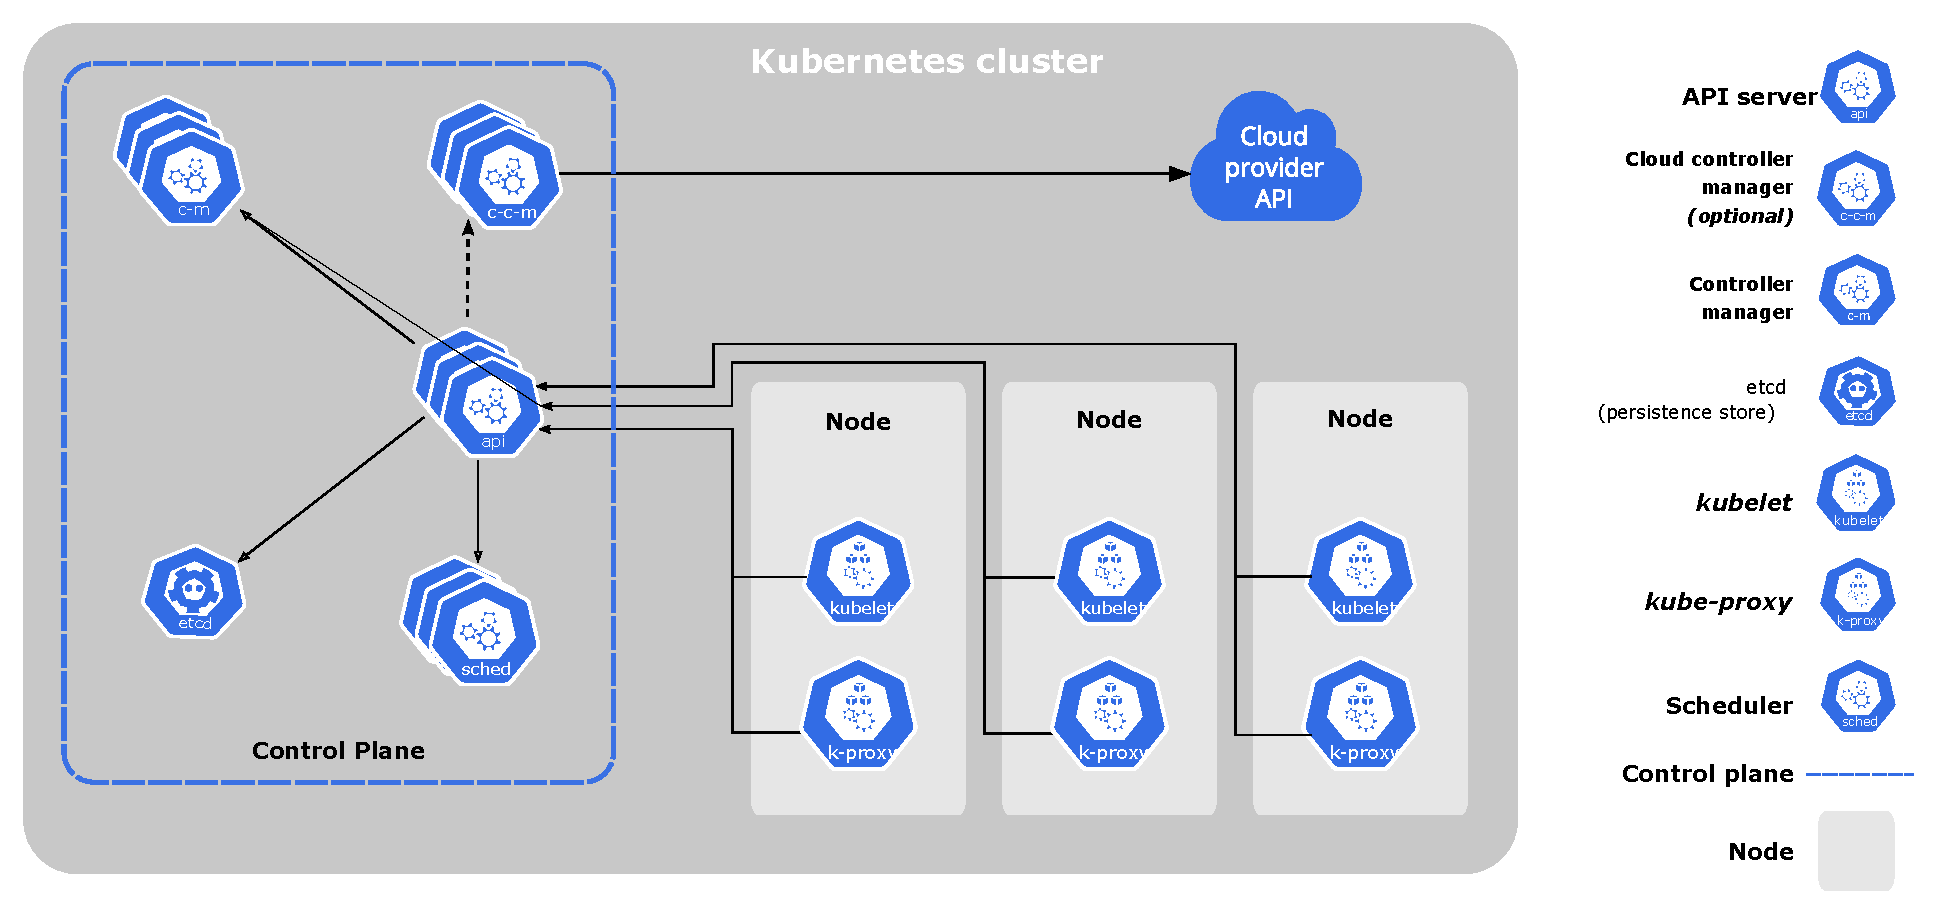
\includegraphics[width=\textwidth]{images/components-of-kubernetes.pdf}
    \caption{The components of a Kubernetes cluster~\cite{kubernetes-components}}
    \label{kube-components}
\end{figure}

A Kubernetes cluster consists of a control plane and one or more worker Nodes.
Components in the control plane manage the overall state of the cluster. The
\verb|kube-apiserver| exposes the Kubernetes HTTP API, which is used to publish
objects such as Deployments, DaemonSets and Jobs. Each
Node in the cluster contains a \verb|kubelet| which manages Pods and ensures
they and their containers are running via a container runtime.

Kubernetes objects are persistent entities in the Kubernetes system. They act as
``records of intent" and describe the cluster's desired state: once created, the
Kubernetes system will constantly work to ensure that the objects exists. The
Kubernetes API is used to create, modify or delete these Kubernetes objects. Almost
every Kubernetes object includes two fields: \verb|spec| and \verb|status|.
\verb|spec| is used on creation as a description of the Objects desired state.
Users can define affinities and QoS classes within this field to influence
scheduling decisions. Containers also contain a \verb|spec| field which
specifies \verb|request| and \verb|limits|. The \texttt{request} field behaves
as a set of minimum requirements and is used when scheduling Pods. In contrast,
the \texttt{limits} field is used by kernel of the Node to throttle a
container's resource usage. \verb|status| describes the current state of the
object, supplied and updated by the Kubernetes system. These fields are core to
scheduling in Kubernetes.

\subsection{Scheduling in Kubernetes}
In Kubernetes, Pods are the smallest deployable units of computing that you can
create and manage. It represents a single instance of a running
process in your cluster and typically contains one or more containers that are
tightly coupled and share resources. Pods can be individually created with their
own Yaml files. However, the Kubernetes API also provides workload objects to
manage multiple pods: these objects represent a higher abstraction level than a
Pod, and the Kubernetes control plane uses the workload's specification to
manage Pod objects on your behalf. Example workloads include Deployment,
StatefulSet, DaemonSet and Job.

When a Pod is created, it initially exists in a ``Pending" state: it has been
declared but hasn't yet been allocated to a Node. Kubernetes schedulers watch for
newly created but unassigned Pods, and based on a set of
rules or algorithms, select the most suitable Node for that Pod. Once a Node is
chosen, the scheduler ``binds" the Pod to the Node, updating the Pod's definition
in the Kubernetes API server by setting its \verb|spec.nodeName| field to the
name of the Node. Once this occurs, the Pod transitions from ``Pending" to
``Running".

\section{\protect\textsc{Pronto}}

\subsection{Principle Component Analysis}
This section first explains Singular Value Decomposition (SVD) and how it
relates to solutions of Principal Component Analysis (PCA). I then introduce
Incremental-SVD and Subspace-Merge, which are used to perform FPCA on the stream
of telemetry produced by each Node.

\subsection{Singular Value Decomposition}
The SVD of a real matrix $\mathbf{A}$ with $m$ rows and $n$ columns where $m
\geq n$ is defines as $\mathbf{A} = \mathbf{U}\Sigma\mathbf{V}^T$. Here, $\mathbf{U}$ and
$\mathbf{V}$ are orthogonal matrices of shape $m \times m$ and $n \times n$
containing the left and right singular vectors, respectively. $\Sigma$ is a
rectangular matrix of shape $m \times n$ with singular values $\sigma_i$ along
its diagonal~\cite{Strang2009}.
\begin{align}
\mathbf{A} = \begin{bmatrix} a_{11} & \dots & a_{1n} \\ \vdots & \ddots & \vdots
    \\ a_{m1} & \dots & a_{mn} \end{bmatrix} = \begin{bmatrix} \mid & & \mid \\ u_1 & \ldots & u_m
\\ \mid & & \mid  \end{bmatrix} \begin{bmatrix} \sigma_1 & &  & \mid & & \mid \\ &
\ddots & & 0 & \ldots & 0 \\ & & \sigma_m & \mid & & \mid  \end{bmatrix} \begin{bmatrix}
    \text{---} & v_1^T & \text{---} \\ & \vdots & \\ \text{---} & v_m^T & \text{---} \\
    \text{---} & v_{m+1}^T & \text{---} \\ & \vdots  & \\ \text{---} & v_n^T & \text{---}
\end{bmatrix}
\end{align}

SVD can also be written compactly by discarding the elements which do not
contribute to $\mathbf{A}$.
\begin{align}
\mathbf{A} = \begin{bmatrix} \mid & & \mid \\ u_1 & \ldots & u_m
\\ \mid & & \mid  \end{bmatrix} \begin{bmatrix} \sigma_1 &
        & \\ & \ddots & \\ & & \sigma_m \end{bmatrix} \begin{bmatrix} \text{---}
& v_1^T & \text{---} \\ & \vdots & \\ \text{---} & v_m^T & \text{---}
\end{bmatrix}
\end{align}

There always exists the SVD for a real matrix, but the decomposition is not
unique: if $\mathbf{A} = \mathbf{U}_1\Sigma\mathbf{V}_1^T =
\mathbf{U}_2\Sigma\mathbf{V}_2^T$ then $\Sigma_1 = \Sigma_2$ but $\mathbf{U}_1 =
\mathbf{U}_2\mathbf{B}_a$ and $\mathbf{V}_1 = \mathbf{V}_2\mathbf{B}_b$ for some
block diagonal unitary matrices $\mathbf{B}_a,
\mathbf{B}_b$~\cite{eftekhari2019moses, Strang2009}. Each column in
$\mathbf{U}$ and $\mathbf{V}$ is an eigenvector of $\mathbf{AA}^T$ and
$\mathbf{A}^T\mathbf{A}$.

\subsection{Principal Component Analysis}
Principal Component Analysis is a staple of linear dimensionality-reduction
techniques. The standard PCA procedure takes as input a matrix $\mathbf{B}$
representing $n$ columns of data with $m$ dimensions. The matrix is first
mean-centered: $\mathbf{A}_{ij} = (\mathbf{B}_{ij} - \mu_i)$ where $\mu_i$ is
the mean of the row $i$. The output of PCA is a set of vectors that explain most
of the variance within $\mathbf{B}$. Given the covariance of the mean-centered
matrix $\mathbf{A}$ is defined as $\mathbf{AA}^T$, the Principal Components (PCs)
maximise the following equation:
\begin{align}
\text{Var}_i = \max_{\substack{x_i \in \mathbb{R}^m \setminus \{\mathbf{0}\} \\
    \|x_i\|=1 \\ x_i \perp x_1 \dots x_{i-1}}} x_i^T \mathbf{A} \mathbf{A}^T x_i
\end{align}

As $\mathbf{A} = \mathbf{U}\Sigma\mathbf{V}^T$ from SVD,
$\mathbf{AA}^T = \mathbf{U}\Sigma\mathbf{V}^T\mathbf{V}\Sigma\mathbf{U}^T =
\mathbf{U}\Sigma^2\mathbf{U}^T$. Therefore, it can be shown that the PCs
$x_i = u_i$ from $\mathbf{U}$. The pair $\mathbf{U}, \Sigma$ will also be
referred to as a subspace as they provide sufficient information to describe the
original $\mathbf{B}$ matrix.

\subsection{Subspace-Merge}
Subspace-Merge is used to merge two subspaces together. Given two subspaces
$(\mathbf{U}_1, \Sigma_1)$ and $(\mathbf{U}_2, \Sigma_2)$ from $\mathbf{Y}_1$ and
$\mathbf{Y}_2$ respectively, the subspace of $\mathbf{Y} = [\mathbf{Y}_1,
\mathbf{Y}_2]$ is:
\begin{align}
    \mathbf{U}\Sigma = \text{SVD}([\mathbf{U}_1\Sigma_1, \mathbf{U}_2\Sigma_2])
\end{align}
$[\mathbf{A}, \mathbf{B}]$ signifies the concatenation of two matrices with the
same number of rows.

\subsection{Incremental-SVD}
Incremental-SVD allows \textsc{Pronto} to become a streaming algorithm with limited
memory. It takes a stream of chunks $\mathbf{Y}_i$, such that  $[\mathbf{Y}_1,
\ldots, \mathbf{Y}_l] = \mathbf{Y}$, and with each recieved chunk it performs
Subspace-Merge to produce $\mathbf{U}_l, \Sigma_l$ where $\mathbf{Y} =
\mathbf{U}_l\Sigma_l\mathbf{V}_l^T$

\begin{algorithm}
\caption{Incremental-SVD}
\textbf{Data:} $\mathbf{Y} = [\mathbf{Y}_1, \dots, \mathbf{Y}_l]$ \\
    \textbf{Result:} $\mathbf{U}_l, \Sigma_l$ such that $\mathbf{Y} =
    \mathbf{U}\Sigma\mathbf{V}^T$
\begin{algorithmic}
\State $\mathbf{U}_1, \Sigma_1, \mathbf{V}_1^T = \text{SVD}(\mathbf{Y}_1)$
\For {$i = 2$ to $l$}
\State $\mathbf{U}_i, \Sigma_i, \mathbf{V}_i^T = \text{SVD}([\mathbf{U}_{i-1}\Sigma_{i-1}, \mathbf{Y}_i])$
\EndFor
\end{algorithmic}
\end{algorithm}
If the shape of the batches of data is $m \times b$, the space complexity of
Incremental-SVD is $\mathcal{O}(m^2 + mb)$ as only the latest version of
$\mathbf{U}_i,\Sigma_i$ and $\mathbf{Y}_i$ are needed for each iteration.

\subsection{FPCA and FSVD}
FPCA combines the relationship between standard SVD and PCA with the
Subspace-Merge operation, to calculate the PCs of the data $[\mathbf{Y}_1,
\ldots,\mathbf{Y}_m]$ from $m$ nodes. Every node $i$ performs perform SVD  on
their local data, to produce the subspace $\mathbf{U}_i, \Sigma_i$. These
subspaces can be merged using at most $m-1$ Subspace-Merges to obtain the global
subspace $\mathbf{U}'\Sigma'$, corresponding to the PCs of the aggregated data
from all the nodes. \textsc{Pronto} turns this procedure into a streaming algorithm, by
running Subspace-Merge on the subspaces produced by incremental-SVD. Finally,
\textsc{Pronto} also introduces a forgetting factor $\gamma$ in front of
$\mathbf{U}_i\Sigma_i$ in Incremental-SVD that allows it to ``forget" old data
by gradually reducing the influence of previous subspaces. Like with standard
PCA, FPCA can be considered as FSVD on mean-centered data.

\subsection{Low-Rank Approximations}
It can be shown that using the first $r$ eignenvectors in the above algorithms
approximate the result of using all $m$ eignenvectors, i.e. if
\begin{align}
\mathbf{Y} = \begin{bmatrix} \mid & & \mid \\ u_1 & \ldots & u_m
    \\ \mid & & \mid  \end{bmatrix} \begin{bmatrix} \sigma_1 &
        & \\ & \ddots & \\ & & \sigma_m \end{bmatrix} \begin{bmatrix} \text{---}
& v_1^T & \text{---} \\ & \vdots & \\ \text{---} & v_m^T & \text{---}
\end{bmatrix}
\end{align}
We can use $\mathbf{U}^r = \begin{bmatrix} \mid & & \mid \\ u_1 & \ldots & u_r
    \\ \mid & & \mid  \end{bmatrix}$ and $\mathbf{\Sigma}^r = \begin{bmatrix}
\sigma_1 & & \\ & \ddots & \\ & & \sigma_r \end{bmatrix}$ where $r \leq m$ in
Incremental-SVD and Subspace-Merge. This lets \textsc{Pronto} reduce the number of
computations it performs and its memory usage.

\subsection{\protect\textsc{Pronto} System Overview}
\begin{figure}[ht]
    \centering
    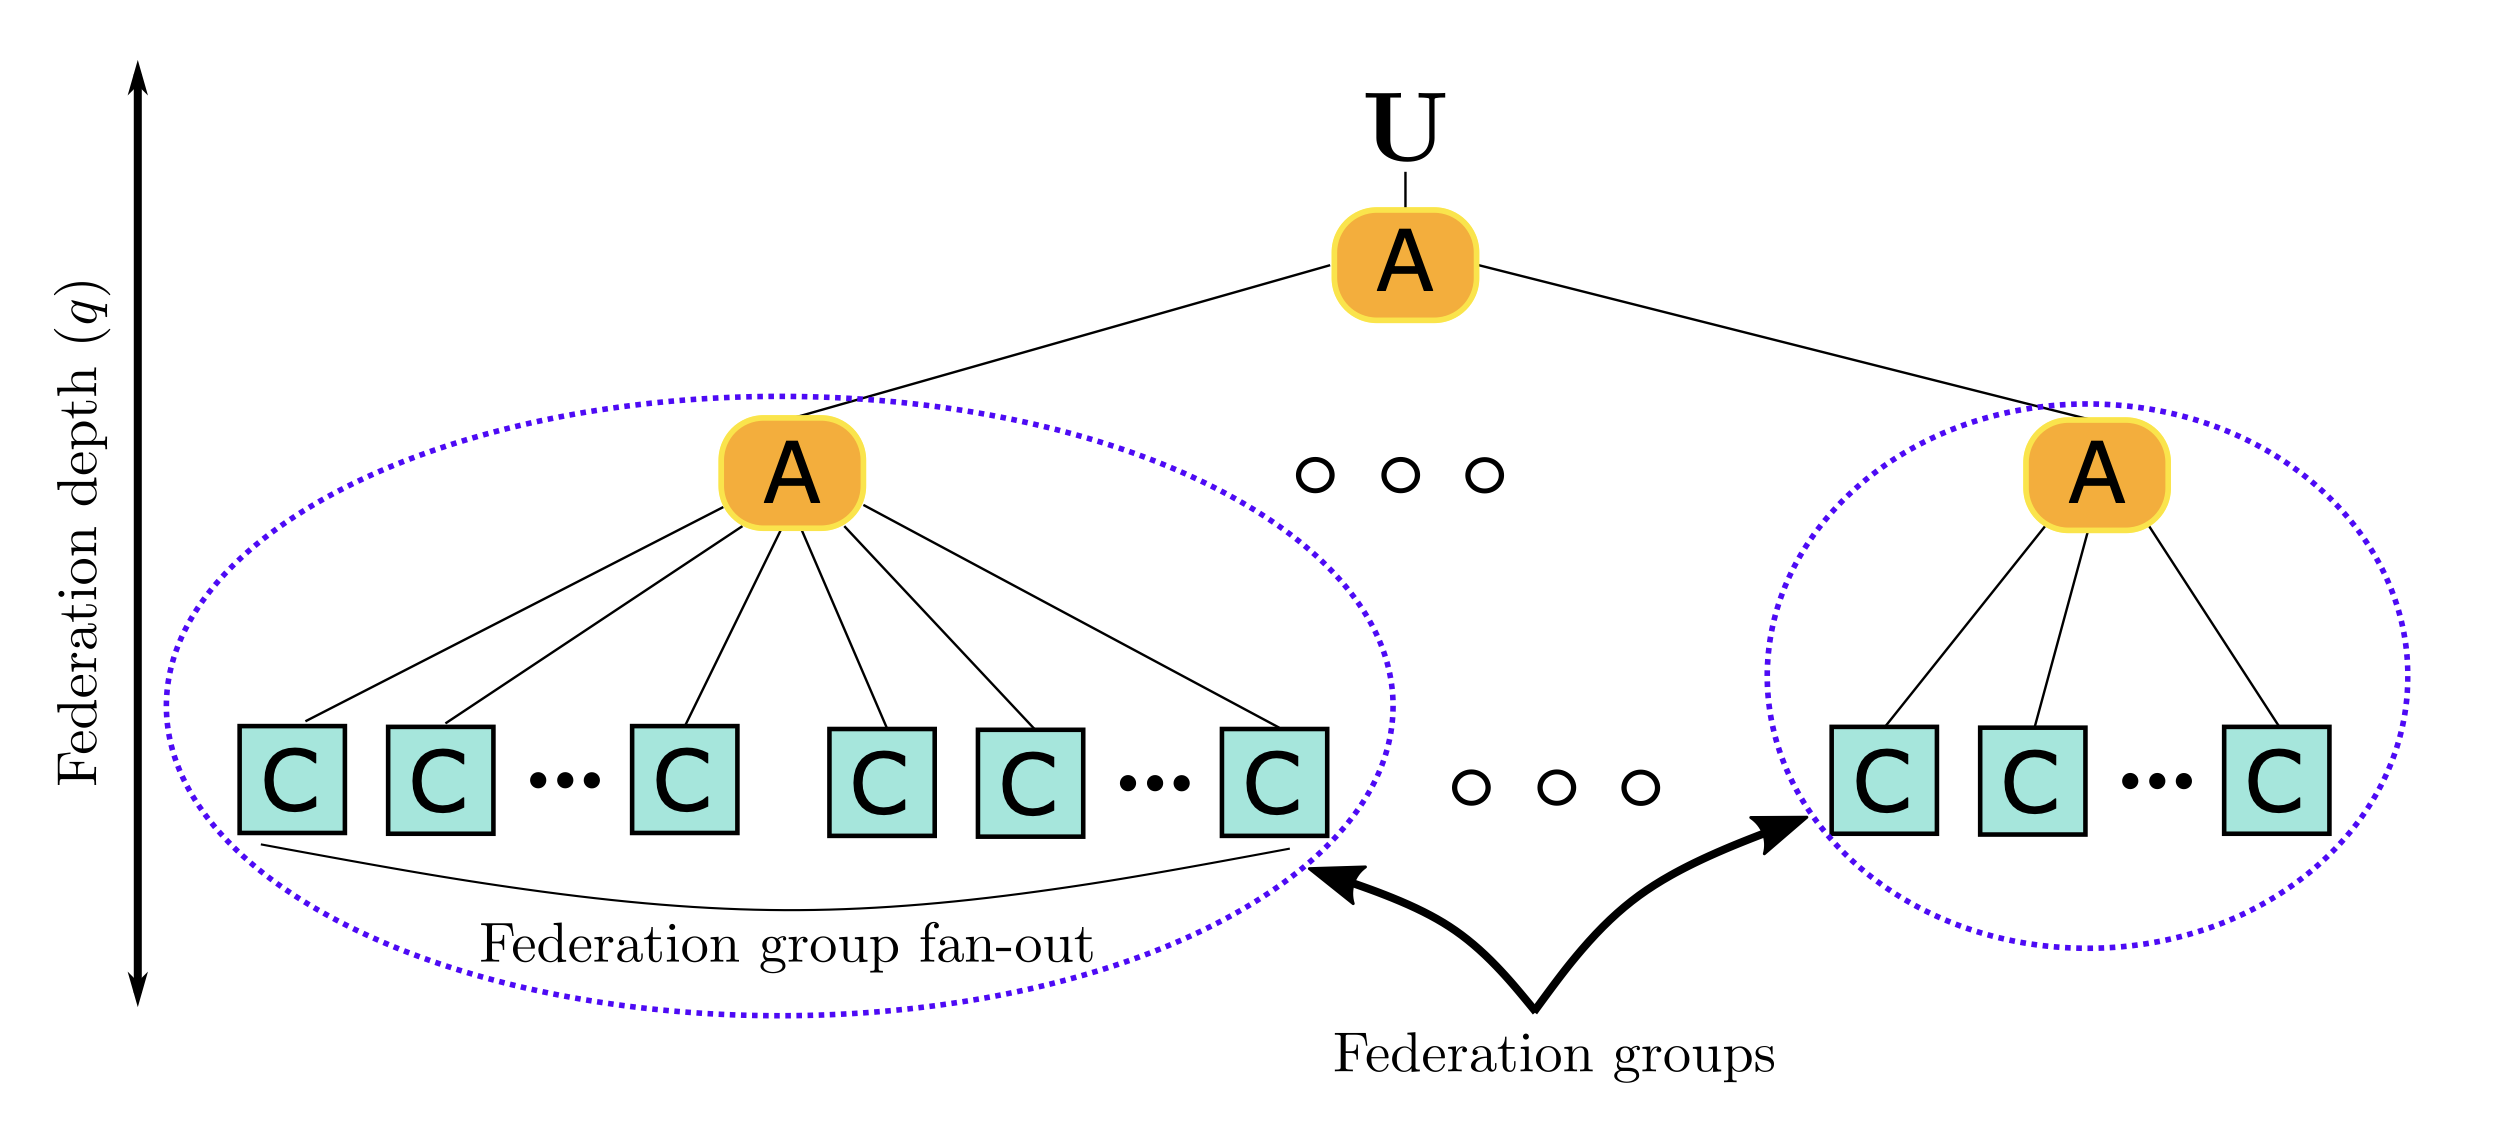
\includegraphics[width=\textwidth]{images/pronto-agg.png}
    \caption{How local models are aggregated in \textsc{Pronto}. Dedicated aggregator
    nodes propagate the updated subspaces until the root is reached~\cite{grammenos_pronto_2021}.}
    \label{pronto-agg}
\end{figure}
There are two types of nodes in \textsc{Pronto}: compute node (C) and aggregator node
(A). Compute nodes collect and center node statistics (i.e. CPU and Memory) and
perform Incremental-SVD to obtain the low rank approximations of the local
subspace $\mathbf{U},\Sigma$. The aggregator nodes perform Subspace-Merge on
incoming subspaces, with subspace produced by the root aggregator node being
propagated back to the compute nodes.

\subsection{\protect\textsc{Pronto} Reject-Job Signal}
\begin{figure}[ht]
    \centering
    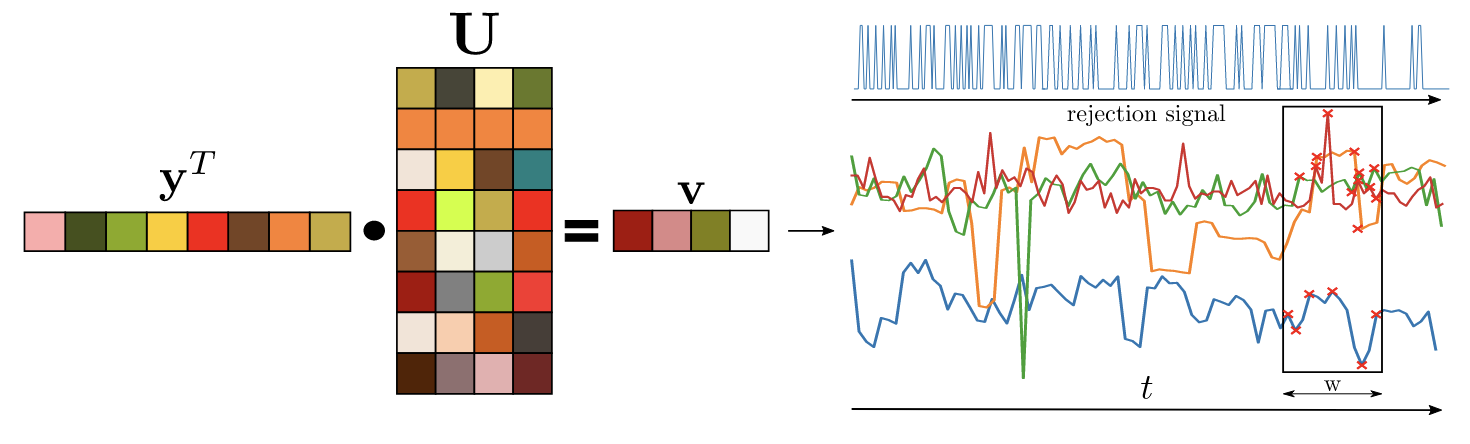
\includegraphics[width=\textwidth]{images/pronto}
    \caption{Projection of incoming $y \in \mathbb{R}^d$ onto embedding $U \in
    \mathbb{R}^{d \times r}$ producing $R$ projections in $v \in \mathbb{R}^{1
    \times r}$. Projections are tracked over time for detecting spikes which
    form the basis of the rejection signal. The sliding window for spike
    detection for each projection is of size $w$ also shown in the figure.}
    \label{pronto-components}
\end{figure}

Each compute node projects their data onto the latest version of $\textbf{U}$,
and identifies all the spikes. If the weighted sum of these spikes, using the
corresponding singular values in $\Sigma$, exceeds a threshold, a rejection
signal is raised to indicate that the node is potentially experiencing
performance degradation and a job should not be scheduled on that node.

\subsection{Strengths}
\textsc{Pronto}'s core strength is its ability to leverage global telemetry data
to predict performance degradation with high accuracy. The orginal
\textsc{Pronto} paper~\cite{grammenos_pronto_2021}, which compared its
effectiveness against non-distributed dimensionality-reduction methods,
demonstrated superior performance in predicting CPU-Ready spikes in real-world
datacenter traces. This improved accuracy over the non-distributed
strategies suggests that significant correlations exist between the resource
usages of different jobs across various nodes at the same point in time. This
federated approach allows for a more comprehensive understanding of system-wide
resource contention, providing more accurate contention predictions than with
only individual node data. These compelling results indicate a strong potential
benefit from applying \textsc{Pronto} underlying principles to a Kubernetes
environment where efficient resource management is paramount.

\subsection{Weaknesses}
\label{sec:intro-weakness}
While \textsc{Pronto} offers a promising approach to performance prediction, its
direct application within Kubernetes scheduling environment faces significant
challenges due to fundamental assumptions and practical limitations of its
original design.

\subsubsection{Assumptions}
The \textsc{Pronto} paper primarily focuses on a method for measuring node
"responsiveness" to future workloads, yielding a binary Reject-Job signal.
However, implementing its design in a complex system like Kubernetes raises
fundamental challenges:
\begin{enumerate}
    \item \textbf{Zero-Latency Assumption:} A critical assumption in the
        \textsc{Pronto} paper is the absence of communication latency, and
        implicitly binding latency within the system. This implies that
        scheduled workloads are immediately reflected in the telemetry, and thus
        the signal. In such a scenario, a central scheduler could
        instantaneously stop assigning workloads once a Node signal potential
        degredation. However, this assumption does not hold in real-world
        Kubernetes clusters. The latency between a pod being bound to a Node and
        that Pod actually starting to run and consume resources has been shown
        to reach as high as 4 seconds \cite{qadeer_scaling_2022}. Directly
        applying \textsc{Pronto}'s binary signal in this high-latency
        environment could lead to a ``runaway train" schenario": Nodes might
        advertise willingness to accept new Pods while a large number of
        ``inflight" Pods are still pending startup and will overload the node
        once active.
    \item \textbf{Lack of Explicit Allocation Algorithm:} \textsc{Pronto} allows
        individual compute nodes to reject or accept incoming jobs. However, it
        does not explicitly provide a system to optimally decide which compute
        nodes are considered for a task. While a simple approach would be to allow
        individual Nodes to request Pending Pods, it suffers from scalability
        issues as hundreds of Nodes sending requests to the Kubernetes APIServer
        would greatly degrade its performance or even cause it to crash.
        Instead, I decided to take a centralised approach, where Nodes
        periodically update their signal to influence where Pods are allocated.
    \item \textbf{Limited Scoring Capability:} Unlike typical Kubernetes
        schedulers that employ a scoring-function to rank Nodes and select the
        ``optimal" fit~\cite{kube-scheduler}, a binary signal offers no
        mechanism to differentiate between suitable Nodes. This could lead to
        suboptimal allocation decisions, potentially reducing overall cluster
        throughput and efficiency
\end{enumerate}
These issues raise the need for a more sophisticated signal that is:
\begin{enumerate}
    \item \textbf{Comparable:} provides enough information to score and rank
        Nodes effectively.
    \item \textbf{Reservable:} allows the scheduler to track the pending impact
        of previous scheduling decisions until Pods have begin running.
\end{enumerate}

% The Pronto paper implements a binary "responsiveness" signal which predicts
% upcoming performance degradation. Because the authors assume a system with no
% communication latency (implicitly assuming that scheduled workloads were
% immediately visisble in the signal as well), they could send this signal
% directly to a central scheduler which could then stop assigning workloads once a
% node sent a Reject Signal.
%
% However, due to significant pod startup latency, the method can't be used in a
% real-world Kubernetes cluster is infeasible. When measuring pod startup in a
% 100 node clusters, the more than 50\% of pods took more than $\approx$ 1 second
% to startup. In addition, when nodes were 100\% full, pod startup could reach up
% to 4 seconds. This latency is significant when Kubernetes schedulers can
% support a throughput of $\approx$1000 pods per second
% \cite{qadeer_scaling_2022}. Applying the same approach as used in the paper,
% could result in nodes advertising a "willingness" to take on new pods while
% a large number of pods are in "flight" and once running will immediately
% overload the node. To prevent this runaway train type problem, I need to define
% a reservation function: a function that reserves an amount of the signal for a
% bound pod. This is necessary to allow previous scheduling decisions to have an
% imnpact on the signal while the signal updates to take into account the
% scheduled pods.
%
% In addition, telemetry-based schedulers can use individual node performance
% information to score and fine-tune pod allocations. A binary signal does not
% provide the necessary information for scoring nodes, potentially resulting in
% worse pod allocations.
%
% In summary, the requirements of the signal are:
% \begin{itemize}
    % \item Reservable: the scheduler must be able to track the pending impact of
        % previous scheduling decisions until the pods have begun running.
    % \item Comparable: the signal must provide enough information to score nodes
% \end{itemize}

\subsubsection{Peak-Prediction}
\textsc{Pronto} relies on peak-detection within contention metrics (originally
CPU-Ready in VMware vSphere) to predict future performance degradation. For
\textsc{Pronto} to generate an accurate Reject-Job signal in Kubernetes, the
chosen contention metrics should exhibit clear, distinguishable spikes during
genuine high-resource contention. While increasing the number of collected
metrics can help reduce the impact of erroneous spikes, collecting more
telemetry and operating on larger matrices will incur additional overheads and
reduce the number of tasks a Node can accept before valid contention is
detected.

Linux-based systems offer Pressure Stall Information (PSI) metrics, accessible
via \texttt{/proc/pressure/<cpu|memory|io>}. These pseudo-files track the time
tasks are stalled waiting for resources. To investigate the feasibility of using
PSI for peak prediction within a Kubernetes Node, I polled the polled the
\verb|/proc/pressure| files under different workloads.

\begin{figure}[ht]
    \centering
    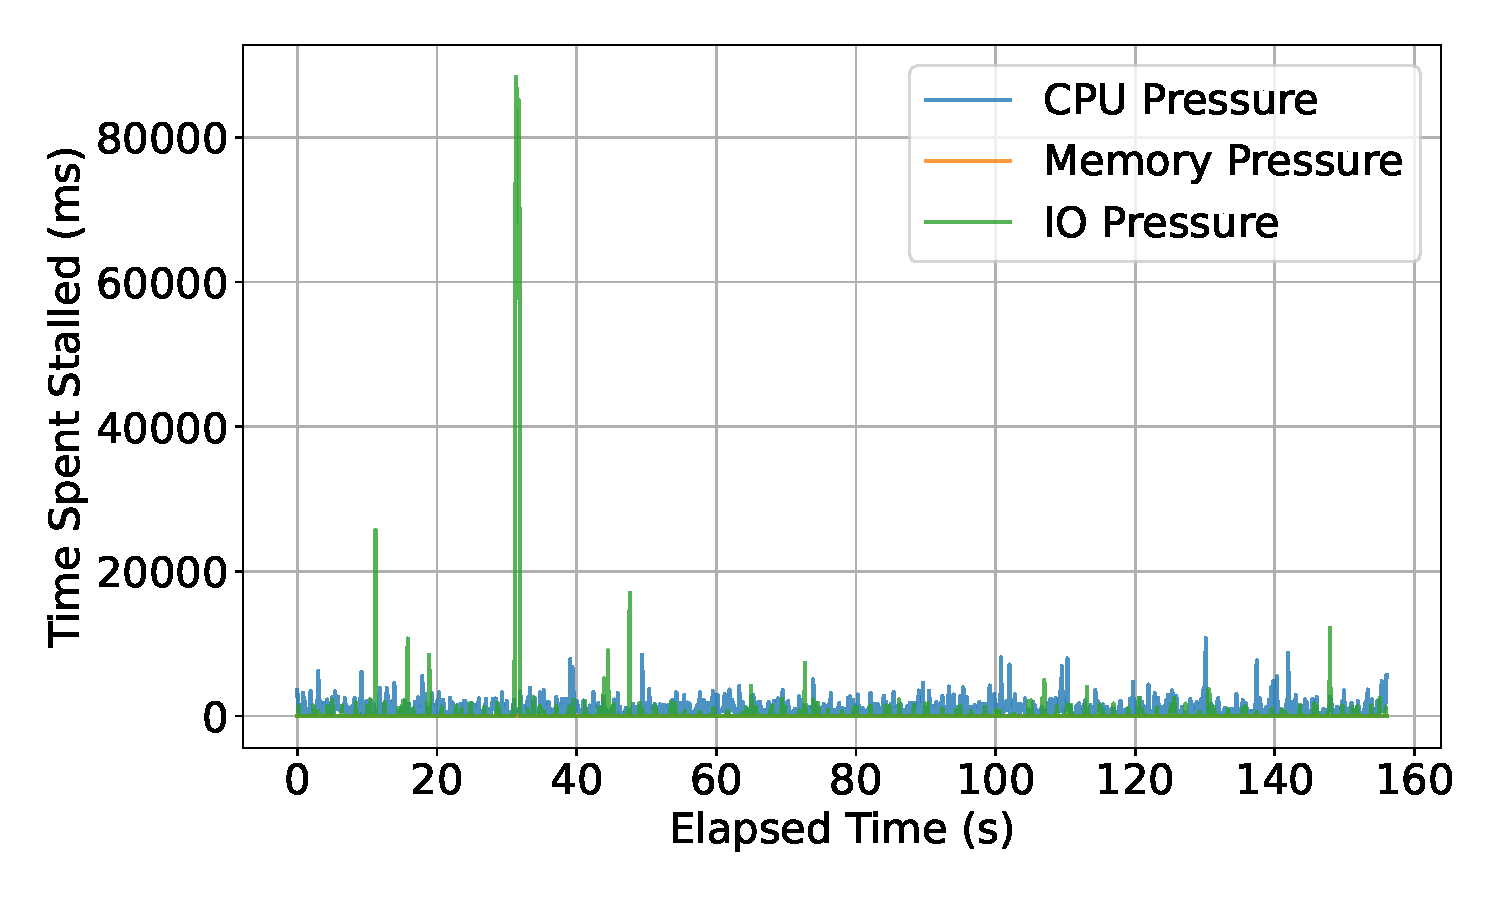
\includegraphics[width=0.48\textwidth]{images/pressure-baseline.pdf}
    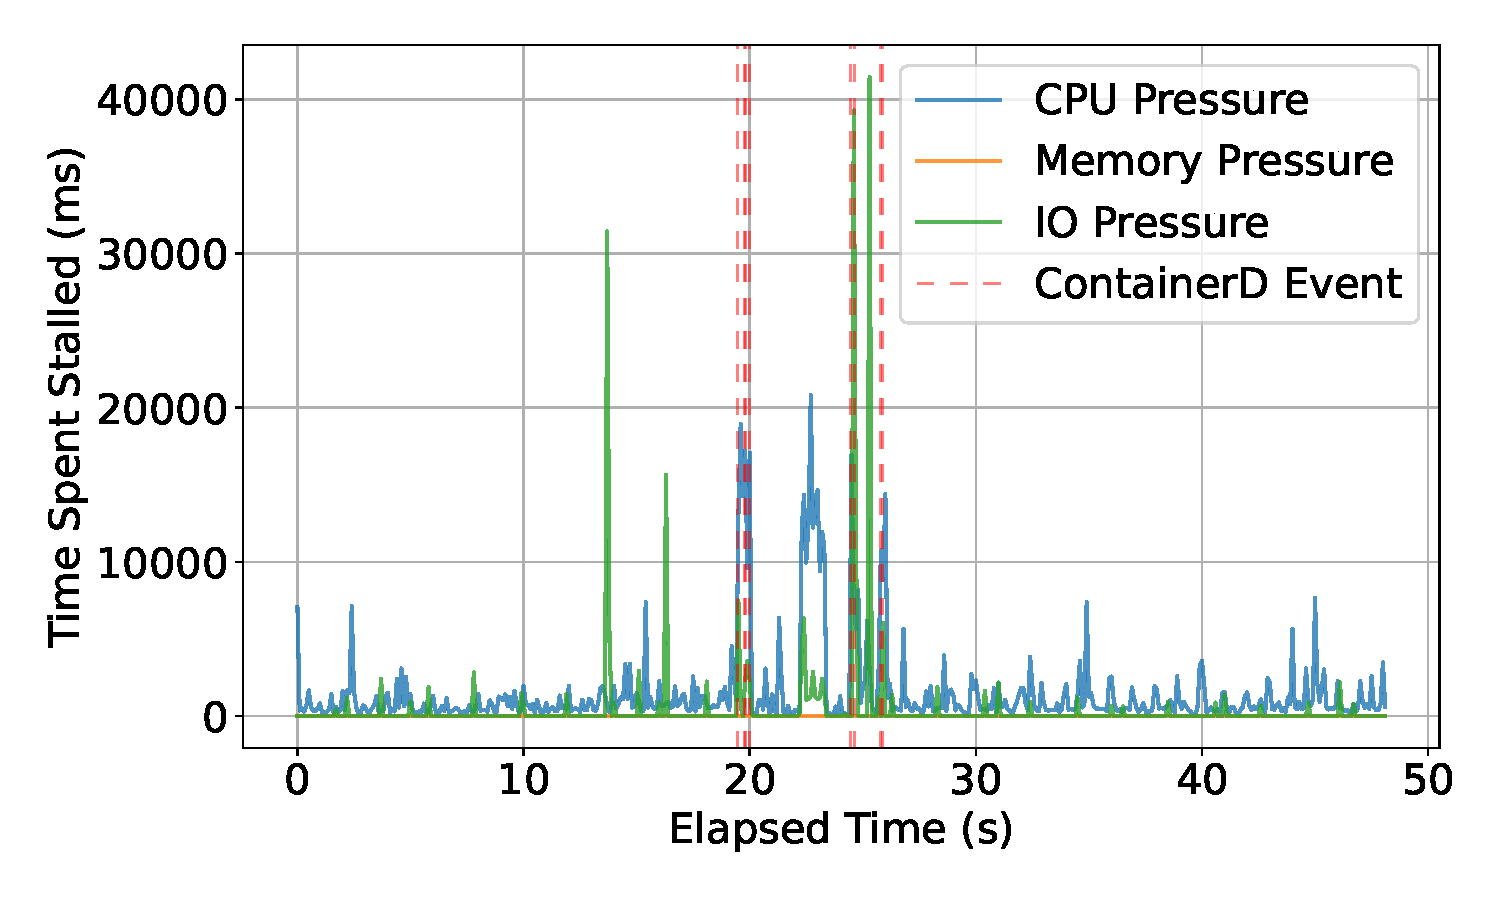
\includegraphics[width=0.48\textwidth]{images/pressure-single.pdf} \\
    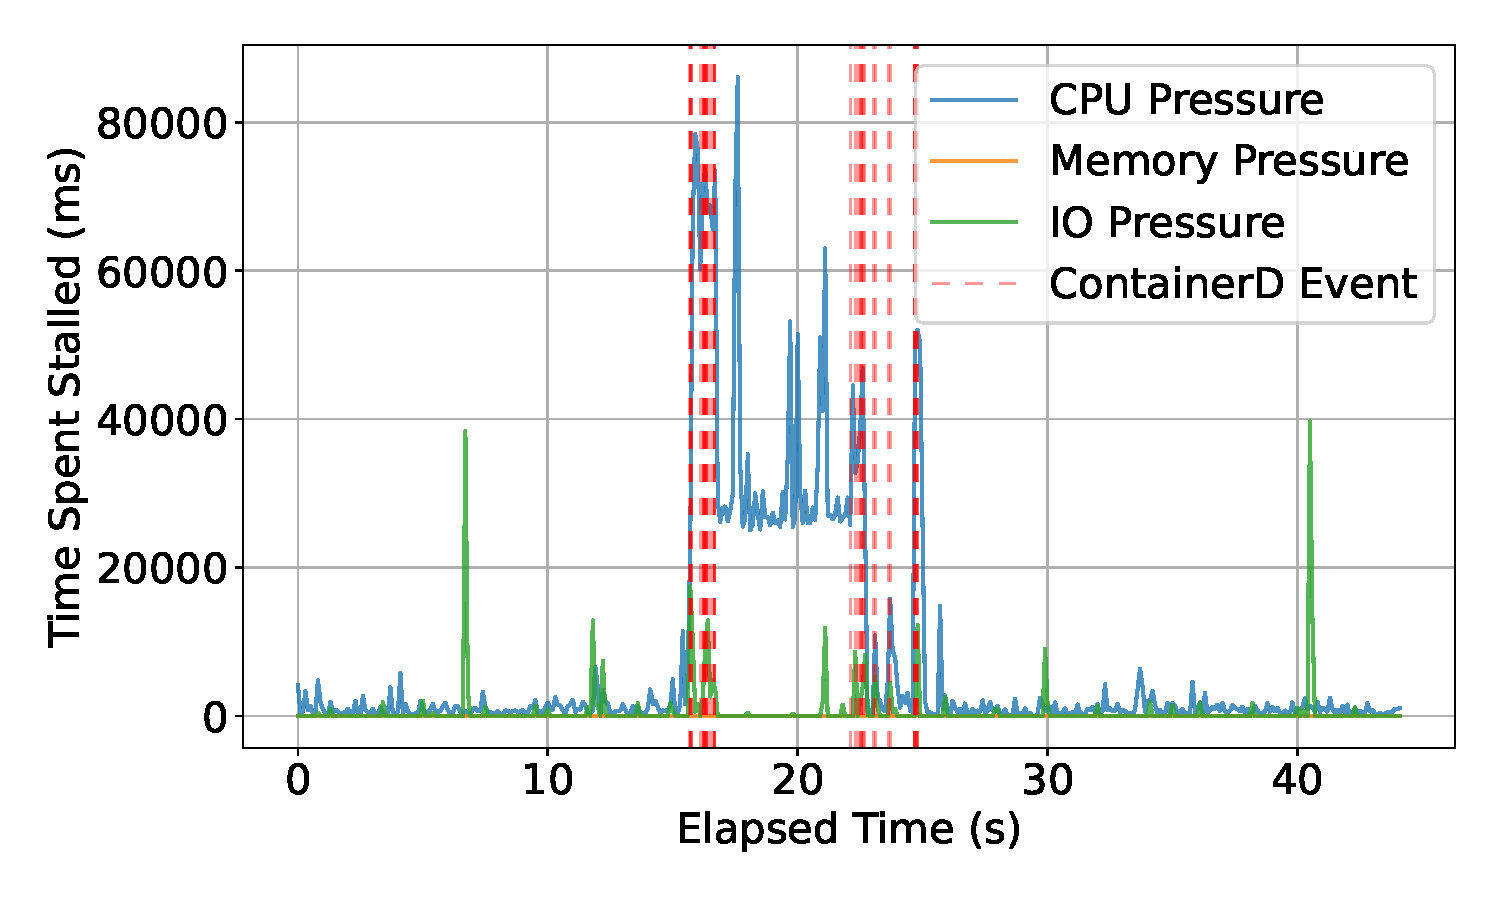
\includegraphics[width=0.48\textwidth]{images/pressure-smallbatch.pdf}
    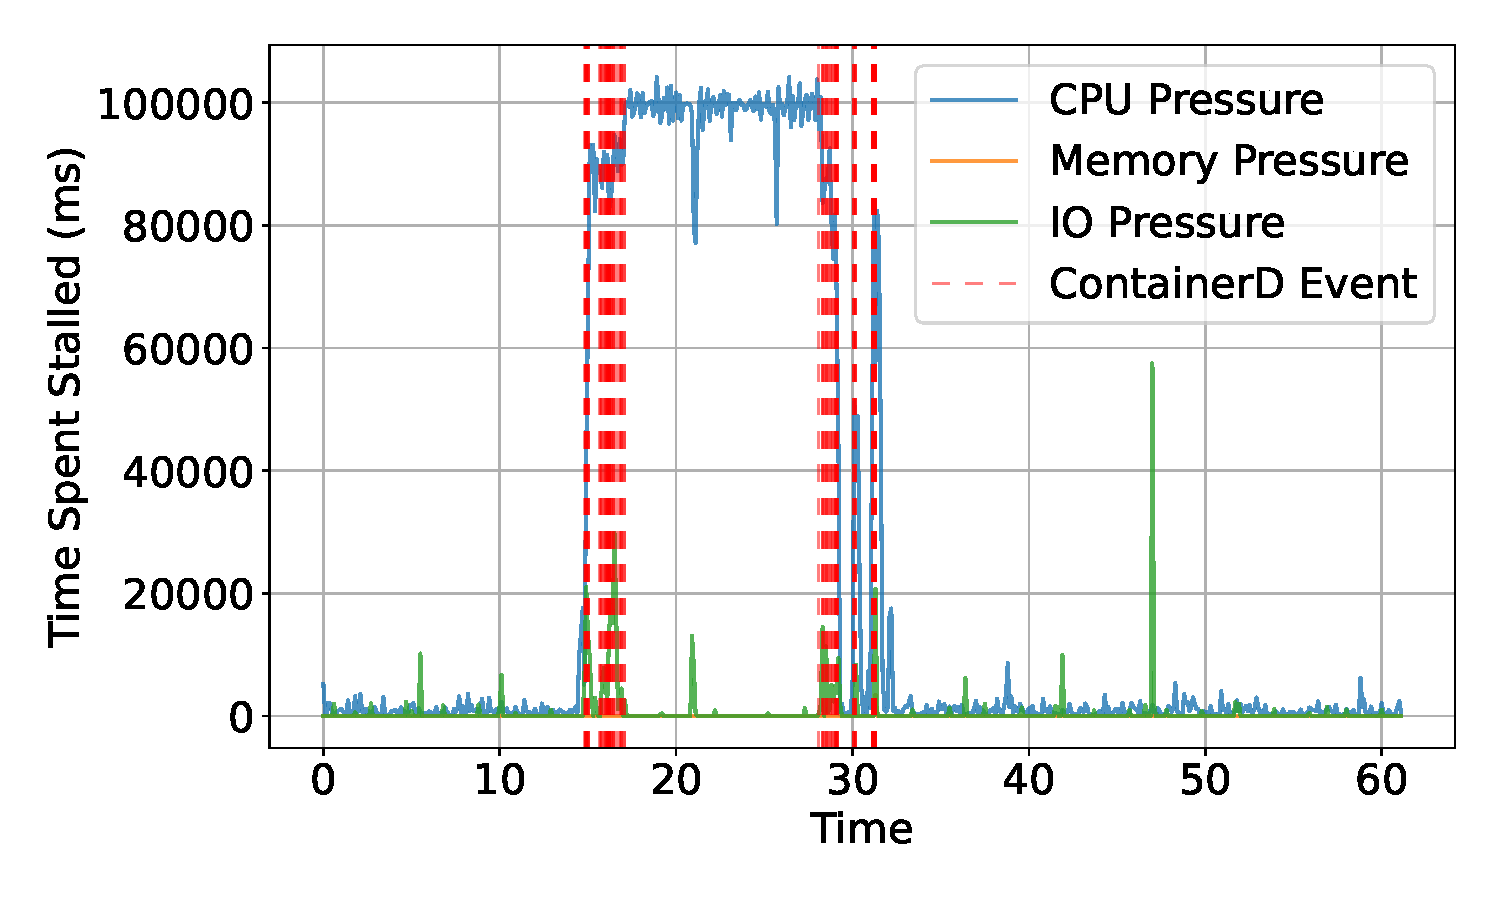
\includegraphics[width=0.48\textwidth]{images/pressure-bigbatch.pdf}
    \caption{Measurements of \texttt{total} from \texttt{/proc/pressure/} under
    different loads. The container runtime results in spikes no matter the
    workload.}
    \label{fig:pressure}
\end{figure}

As demonstrated in Figure \ref{fig:pressure}, even with lightweight workloads,
the PSI metrics frequently experience significant spikes. These transient spikes
can be attributed to the container runtime (e.g. Containerd) consuming resources
during the creation or deleteion of containers. These ``noise" would be
difficult to distinguish from genuine indicators of resource contention ,
compromising the accuracy of \textsc{Pronto}'s peak-detection mechanism.

\begin{figure}[ht]
    \centering
    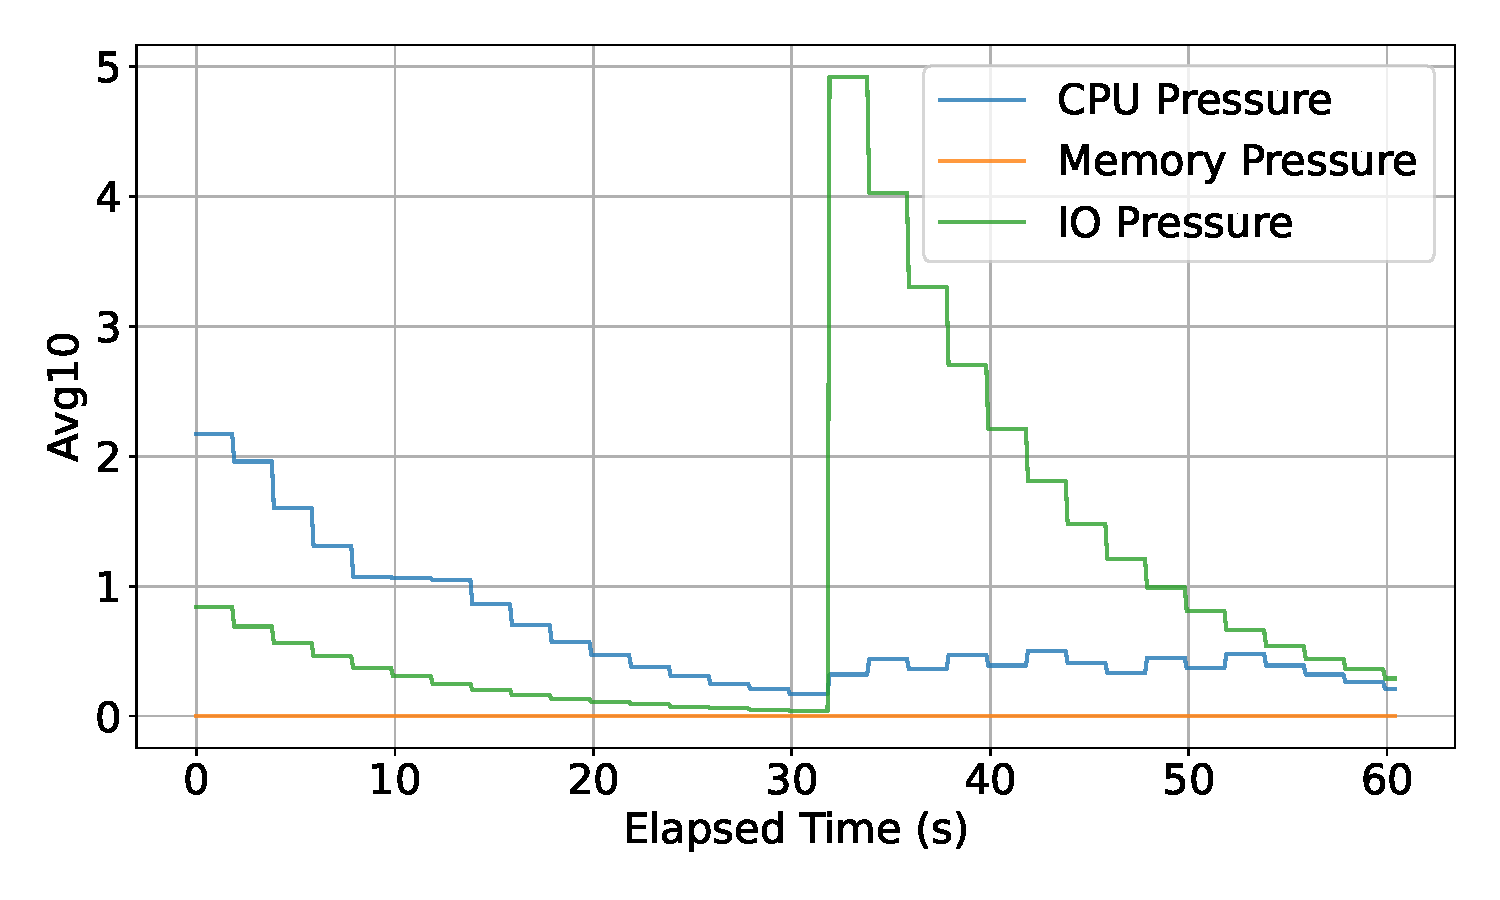
\includegraphics[width=0.48\textwidth]{images/avg-pressure-baseline.pdf}
    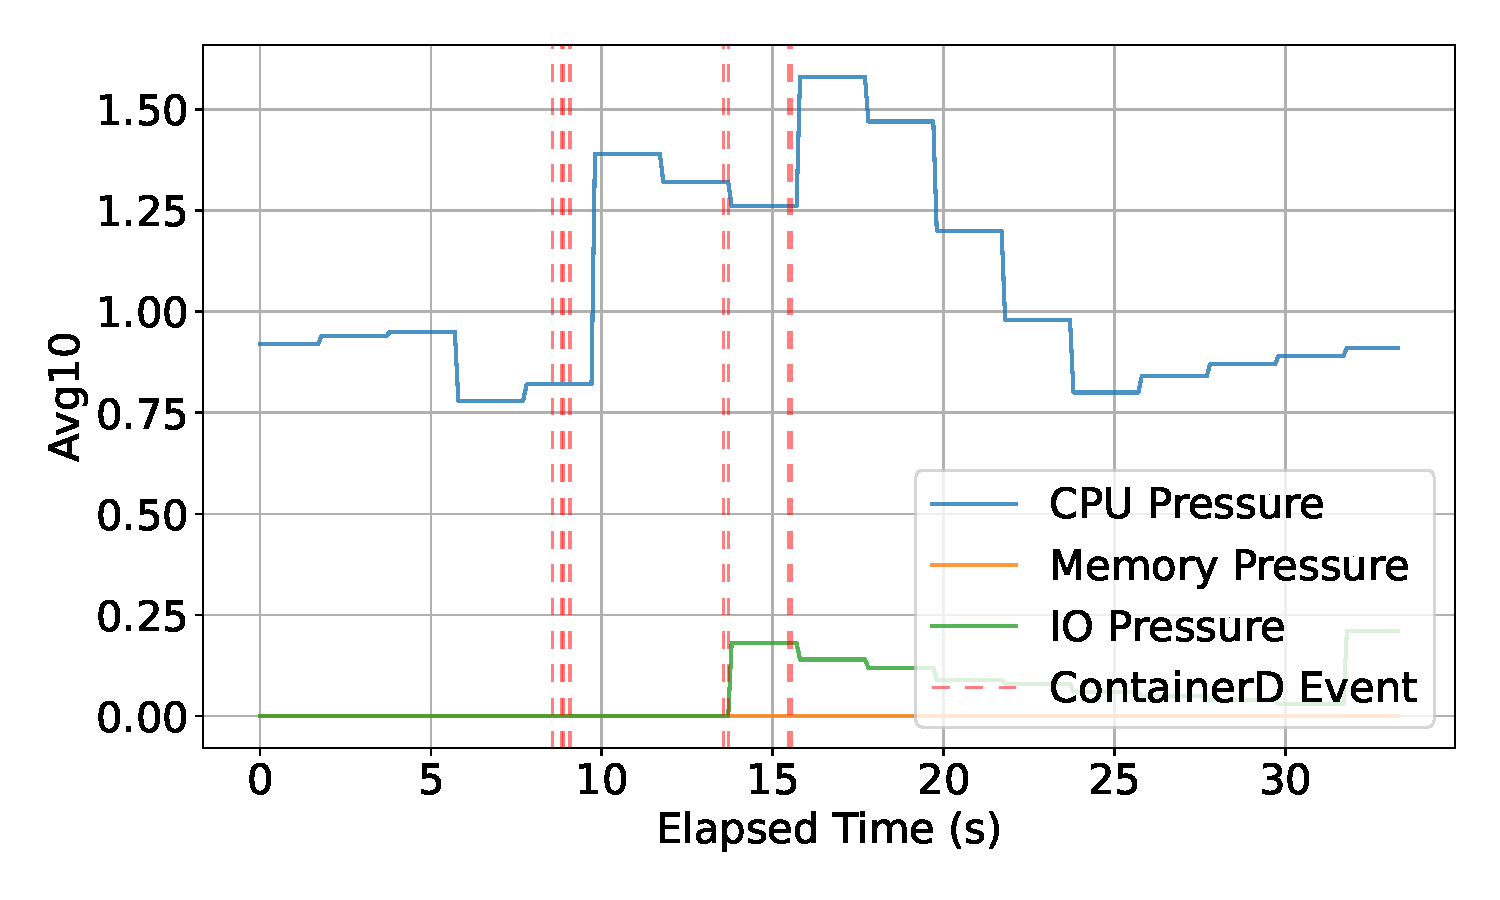
\includegraphics[width=0.48\textwidth]{images/avg-pressure-single.pdf} \\
    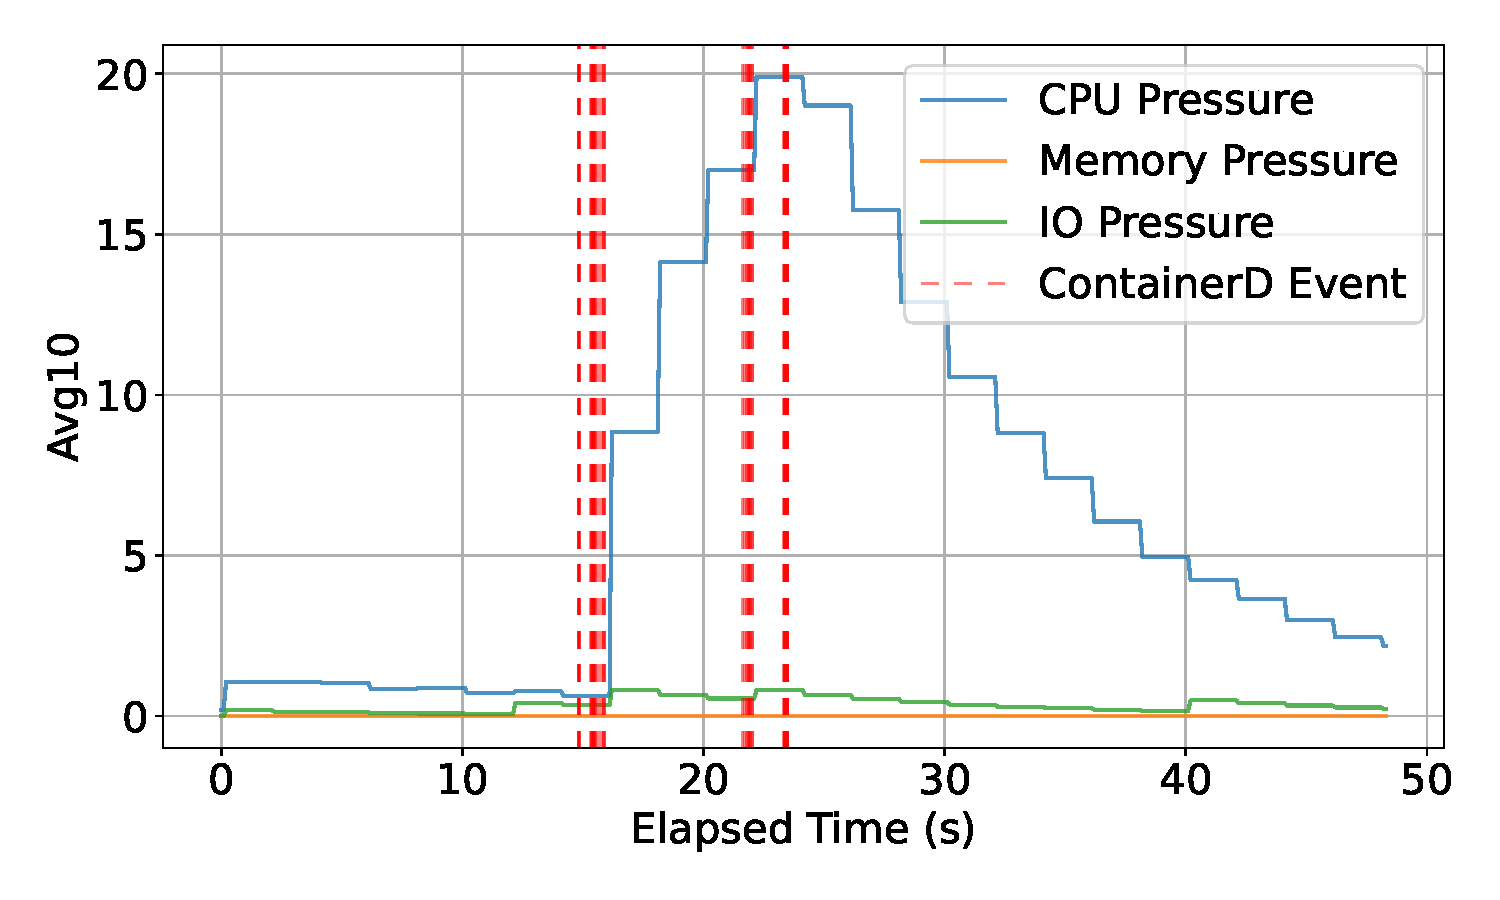
\includegraphics[width=0.48\textwidth]{images/avg-pressure-smallbatch.pdf}
    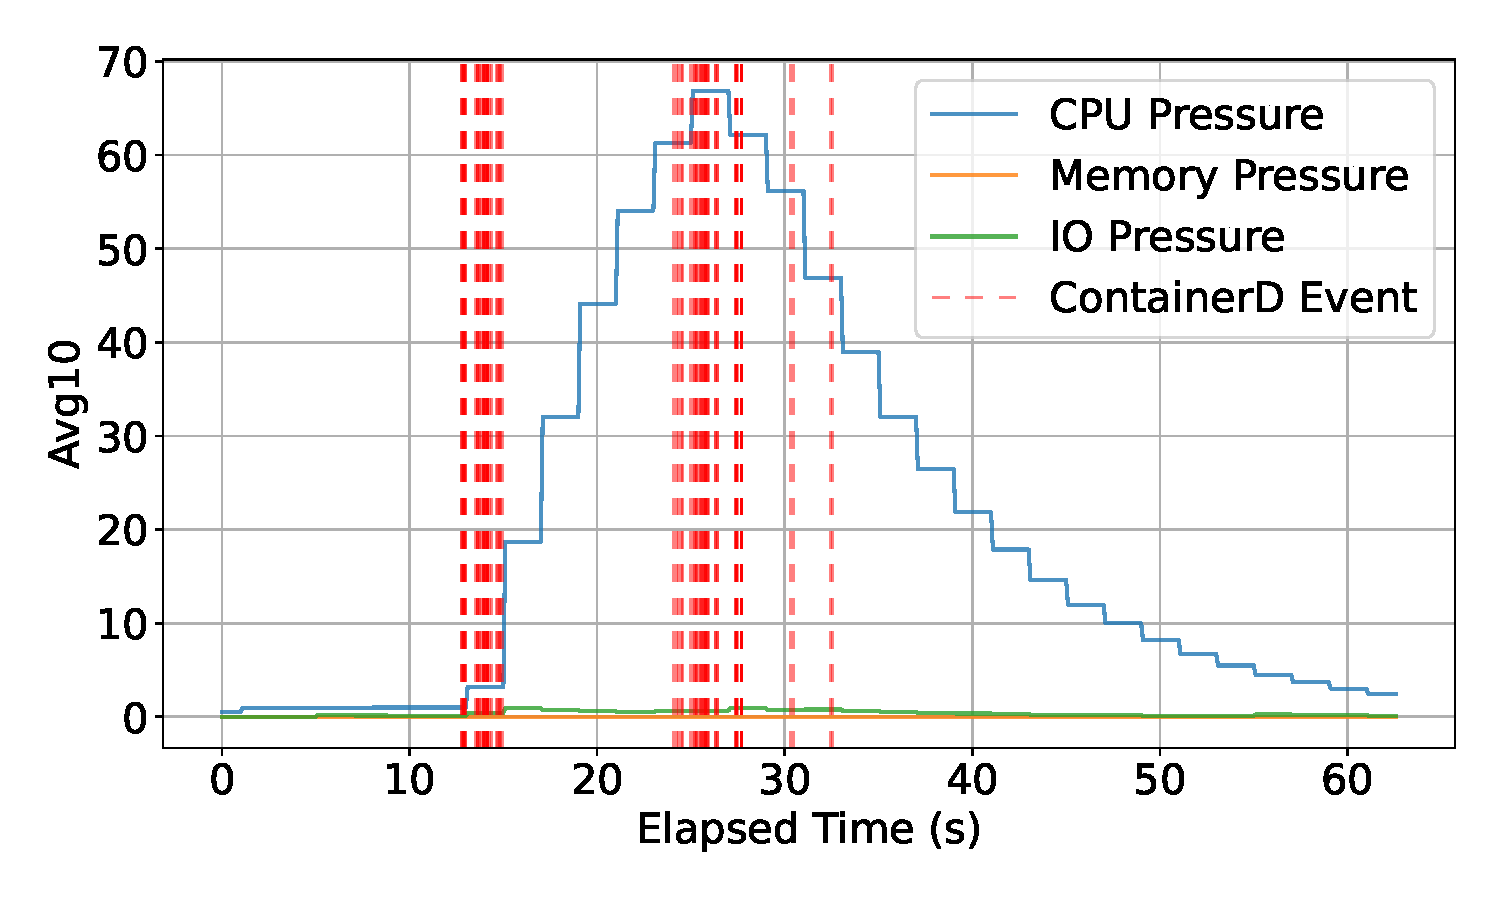
\includegraphics[width=0.48\textwidth]{images/avg-pressure-bigbatch.pdf}
    \caption{Measurements of \texttt{avg10} from \texttt{/proc/pressure/} under
    different loads. The container runtime results in spikes no matter the
    workload.} \label{fig:pressure-avg}
\end{figure}
The PSI metrics also expose an average over a 10-second window. Figure
\ref{fig:pressure-avg} illustrates that averaging the PSI metrics can indeed
reduce the impact of these container runtime-induced spikes. However, this
smoothing comes at the cost of responsiveness. In the experiments with a 10-pod
batch, the averaged metrics failed to converge on the true value observed in
Figure \ref{fig:pressure} before the Pods had finished running. 10 seconds in
the timeframe of Kubernetes can result in the same ``runaway train" situation
described earlier.

Based on this early empirical investigation, I conclude that direct
peak-prediction from sub-second polling of raw PSI metrics, can not be easily
applied within a fast-paced Kubernetes environment.


% In the paper, Pronto uses \verb|CPU-Reeady| which is generated by the VMware
% vSphere virtualisation platform. This metric can't be used within a
% Kubernetes cluster as machines can be both virtual and physical. Since Linux
% 4.20+, the kernel can track how long tasks are stalled waiting for the CPU
% at a cgroup granularity. By inspecting the the root cgroup’s CPU pressure
% file using \verb|cat /proc/pressure/cpu| you can measure the total time all
% processes spent waiting for the CPU to be available.
%
% While this type of metric can be used to alert of performance degradation,
% this metric has a few shortcomings. Firstly, it only reports CPU-centric
% information. This is not always representative measure of resource
% contention as memory-heavy workloads may starve for RAM resources while
% metrics like \verb|CPU-Ready| and \verb|/proc/pressure/cpu| remain
% unaffected.
%
% Secondly, a significant amount of resources are used starting up or deleting
% containers. This results in large spikes, as shown in figure
% \ref{pressure-eval}, which are difficult to distinguish from genuine CPU-Ready
% spikes. As Pronto uses spike detection to predict future resource performance
% degradation, container start-ups could produce detectable spikes which would
% reduce the rate at which pods are assigned to nodes and could result in lower
% throughput.
%


\section{Related Work}
This section examines existing Kubernetes schedulers, highlighting
those that share characteristics with \textsc{Pronto}: distributed and federated
schedulers, online schedulers, performance-aware schedulers, and machine
learning-based schedulers.

\subsection{Federated and Distributed Scheduling}
\textsc{Pronto} is described as a federated algorithm that executes plans in a
decentralised fashion. Each computing node makes independent decisions for task
assignments without needing global synchronisation. This contrasts with
monolithic centralised schedulers~\cite{kube-scheduler, gog_firmament_2016},
such as the default Kubernetes scheduler (\texttt{kube-scheduler}), which acts
as a single dispatcher on the master node and has a global state view. These
schedulers can suffer from scalability issues, reliance on cached data and
increased network traffic~\cite{grammenos_pronto_2021}. Research has been done
in multi-cluster scheduling and cluster federation, addressing challenges in
scalability and geo-distributed environments. Examples include frameworks like
KubeFed~\cite{faticanti2021application} and architectural proposals like
Foggy~\cite{santoro2017foggy}. Although \textsc{Pronto} immediate focus is on
scheudling within a network of nodes that might not be geographically dispersed
or owned by different entities, its federated learning approach to sharing
knowledge through aggregated iterates is relevant to discussions around
decentralised control and coordination in distributed infrastructures.

\subsection{Online, Real-Time, and Streaming Scheduling}
TODO: THIS SECTION FEELS WEAK, I MAY DELETE
\textsc{Pronto} is designed for online task scheduling and operates on real-time
performance. As a streaming algorithm, \textsc{Pronto} processes incoming data
in a single pass without storing historical information, enabling Nodes to make
immediate scheduling decisions about incoming workloads. While the default
Kubernetes scheduler reacts to changes, it performs bin-packing with statically
defined resource requests and capacity. Research outside of Kubernetes has
repeatedly shown that analysing large-scale performance data in near real-time
for efficient scheduling is difficult~\cite{grammenos_pronto_2021}. As a result,
\textsc{Pronto}'s explicit streaming algorithm enabling low-latency scheduling
decisions distinguishes it from approaches that might involve more substantial
processing pipelines, offline techniques or the reliance on potentially stale
cached information.

\subsection{Performance-Aware and Predictive Scheduling}
As a performance-aware scheduler, \textsc{Pronto} employs
dimensionality-reduction technique to efficiently process the vast amount of
telemetry data produced by each node, with the goal of predicting performance
degradation. While, CPU and RAM utilisation are common metrics for
performance-aware Kubernetes schedulers~\cite{bao2019deep, beltre2019kubesphere,
bestari2020dynamic, carvalho2021qoe, toka2021ultra}, \textsc{Pronto}
distinguishes itself as the first scheduler to incorporate CPU-Ready for task
scheduling.

Furthermore, the dynamic nature of Kubernetes workloads strongly suggest that
predictive techniques could improve scheduling efficiency and resource
utilisation~\cite{carrion2022kubernetes}. Traditional forecasting methods (such as
exponential smoothing, ARIMA, and SVM) were also explored in
\cite{grammenos_pronto_2021} for CPU Ready spike prediction, but were found to
have worse accuracy. This still remains an open research topic.

\subsection{Machine Learning-Based Schedulers}
\textsc{Pronto} exploits unsupervised learning technique, specifically Federated
PCA, to discover hidden correlations within unstructured high-dimensional
telemetry data. Machine Learning (ML) algorithms  are increasingly adopted in
scheduling to learn from data and improving decision quality.
Reinforcement learning-based schedulers \cite{bao2019deep, huang2020rlsk,
peng2021dl2, han2021tailored} use reward functions to continuously improve
scheduling decisions. While, ML has been used before to predict application or
resource utilisation~\cite{yang2019design, carvalho2021qoe,
harichane2020proposal}, these schedulers are typically domain-specific.
\textsc{Pronto}'s application of unsupervised PCA to predict the performance
of a Node represents a novel use-case of ML with broad applications within the
scheduling domain.

\subsection{Summary of Related Work}
In summary, \textsc{Pronto} distinguishes itself within the Kubernetes
scheduling landscape through its federated and decentralised approach, enabling
independent decision-making at the node level. Its streaming algorithm allows
for immediate, low-latency task assignments. As a performance-aware scheduler, it
innovatively uses CPU-Ready for task scheduling and applies unsupervised
Federated PCA for predictive insights, offering a distinct machine learning
approach.

\section{Summary}
This chapter provided the foundational knowledge for the dissertation,
introducing an overview of the Kubernetes architecture and its scheduling
mechnaism. It then introduced \textsc{Pronto}, a novel approach to scheduling,
explaining the core mathematics behind its FPCA, and highlighting its accuracy
in predicting performance degradation through global telemetry. However,
significant weaknesses were identified, emphasising the necessity for a more
sophisticated \textbf{comparable} and \textbf{reservable} signal. Finally, a
review of existing Kubernetes schedulers, helped distinguish \textbf{Pronto}
from the current landscape and highlight it potential contribution.

% \begin{tcolorbox}[boxsep=0mm,left=2.5mm,right=2.5mm]
    % \textbf{Summary:} {\em In this chapter I will summarise the problem and
    % problem space. I will review the findings of the related work, highlighting
    % weaknesses of existing Kubernetes schedulesr with respect to QoS
    % scheduling.}
% \end{tcolorbox}



\chapter{\protect\textsc{Carico}}
% This chapter may be called something else\ldots but in general the
% idea is that you have one (or a few) ``meat'' chapters which describe
% the work you did in technical detail.
% \begin{tcolorbox}[boxsep=0mm,left=2.5mm,right=2.5mm]
    % \textbf{Design and Implementation:} {\em In this section, I will outline the
    % goals of my system. I will give a brief overview of the chapter structure,
    % summarising each core section and what I achieve.}
% \end{tcolorbox}
This chapter details \textsc{Carico}, a federated, asynchronous,
memory-limited algorithm, building upon the principles of \textsc{Pronto}.
\textsc{Carico} differentiates itself from \textsc{Pronto} for the following
reasons:
\begin{enumerate}
    \item Rather than performing standard FPCA, \textsc{Carico} applies FSVD on
        observed [0,1]-normalised resource usage. Subsequently, \textsc{Carico} uses
        new interpretations for the results of SVD and modifies the
        Subspace-Merge to preserve the interpretations.
    \item \textsc{Carico} presents a novel continuous and \textbf{comparable}
        capacity signal function that combines the new model interpretations
        with a Node's current resource usage to calculate its estimated
        workload capacity.
    \item \textsc{Carico} makes two assumptions to translate the calculated
        capacity signal into a signal that is both \textbf{reservable} and uses
        the number of Pods as its unit of measure.
\end{enumerate}
As this algorithm produces a signal that measures "capacity", I will refer to it
as \textsc{Carico} - "load" in Italian.

\section{Capacity Signal}
In Section \ref{sec:intro-weakness}, we identified critical limitations of
\textsc{Pronto}'s binary ``Reject-Job" signal within the Kubernetes ecosystem:
its lack of comparable Node scoring and inability to handle Pod start-up
latencies. While one could conceivably compare the number of detected spikes,
it's difficult to quantitatively assign or reserve ``peak detections" for
incoming Pods. Furthermore, as shown in Figure
\ref{fig:podcount-util-pressure}, contention metrics often do not change
proportionally to the number of tasks assigned, making them difficult to
reserve accurately.

These limitations demand a signal reflecting varying levels of contention
and offering a predictable, scalar relationship with task assignments.
\texttt{kube-schedulers}'s reservation of a Node's resource highlights the
potential use of a capacity metric. FPCA's interpretations focus on the
variability within telemetry data rather than its absolute value, and therefore,
is not suitable for calculating measures of capacity. The subsequent
challenge was to find a means of transforming \textsc{Pronto}'s mathematical
framework to produce values that could be interpreted as the direction and
magnitude of recent workload's resource usage. Only once we had this
interpretation, could we then develop a continuous, comparable, and reservable
signal that could effectively and accurately guide scheduling decisions.

\section{Local Model}
\label{sec:local-model-construction}
\textsc{Carico} assumes a batch of telemetric data $\mathbf{A}$ is an $m \times
n$ matrix, where $\mathbf{A}$ contains $n$ samples of $m$-dimensional columns of
data. Each dimension in the vector represents a different resource, where the
value $0$ indicates that full capacity is available for that resource and $1$
indicates that the resource is being fully used ([0,1]-normalised). As we
are no longer mean-centering the dataset before applying SVD, \textbf{PCA's
interpretations no longer apply to the resulting $\mathbf{U}$ and $\Sigma$
matrices}.

Instead, \textsc{Carico} is built on top of  a different set of interpretations.
Using the Lemma proved in Appendix \ref{app:vector-to-avg}, we can interpret the
first left singular vector $u_1$ in $\mathbf{U}$ as a pseudo-weighted average
direction of the datapoints in the matrix: ``larger" or more aligned columns
contribute more significantly to the sum defining $u_1$, and thus to its final
direction. Thus $u_1$ behaves as a primary indicator of the direction of the
current workload's resource usage.

While knowing the proportion of resource usage is useful, it is also important
to be able to differentiate between lightweight workloads and more intense
workloads. For this, \textsc{Carico} uses the first singular value $\sigma_1$ in
$\Sigma$. Given $\sigma_1(\mathbf{A})$ and $u_1$ correspond to the first
singular value and first left singular vector of a batch of telemetry
$\mathbf{A}$:
\begin{align}
    \sigma_1(\mathbf{A})^2 &= u_1^T \mathbf{AA}^T u_1 \\
    &= (u_1^T \mathbf{A})^2
\end{align}
Given $a_j$ is the $j$-th column of $\mathbf{A}$, $\sigma_1(\mathbf{A})^2$ can be
interpreted as the sum of squared scalar projections of columns in $\mathbf{A}$:
$\sigma_1(\mathbf{A})^2 = \sum_{j=1}^n (u^T a_j)^2$.

Furthermore, the first singular value can be shown to scale with resource usage.
Given two batches of telemetry $\mathbf{A}$ and $\mathbf{B}$ where batch
$\mathbf{B}$ experienced more resource usage ($0 \leq a_{ij} \leq b_{ij} \leq 1$
for all $i,j$), it is shown in Appendix \ref{sec:app-monotonicity} that the
first singular value of $\mathbf{B}$ will be greater than or equal to that of
$\mathbf{A}$ ($\sigma_1(\mathbf{A}) \leq \sigma_1(\mathbf{B})$). Subsequently,
the first singular value makes a good indicator of measured resource usage.

\section{Subspace Merging}
\label{sec:local-merge}
While we have shown that the results from performing SVD on [0,1]-normalised
telemetry data can have useful interpretations, the resulting $\sigma_1$ can
grow with each Incremental-SVD (Appendix \ref{sec:app-concatenate}):\\
Given two non-negative matrices $\mathbf{A} \in \mathbb{R}^{m \times n_1}$ and
$\mathbf{B} \in \mathbb{R}^{m \times n_2}$, the first singular value of the
concatenated matrix $\mathbf{C} = [\mathbf{A}, \mathbf{B}]$ is greater than or
equal to the maximum of the first singular values of $\mathbf{A}$ and
$\mathbf{B}$:
\[ \sigma_1([\mathbf{A}, \mathbf{B}]) \geq \max(\sigma_1(\mathbf{A}),
\sigma_1(\mathbf{B})) \]

This property is important, as we established earlier that \textsc{Carico} uses
$\sigma_1$ as an indicator of the magnitude of resource usage. If $\sigma_1$ can
increase while the measured telemetry reports a stable magnitude of resource
usage, its interpretation no longer holds.

To solve this, \textsc{Carico} scales the concatenated matrices using non-negative scalar
weights $\gamma_{\mathbf{A}} = \sqrt{w_{\mathbf{A}}}$ and
$\gamma_{\mathbf{\mathbf{B}}} = \sqrt{w_{\mathbf{\mathbf{B}}}}$ such that
$w_{\mathbf{A}} + w_{\mathbf{\mathbf{B}}} = 1$. This method still preserves the
earlier interpretations:

\begin{itemize}
    \item \textbf{First Left Singular Vector:}\\
        The resulting first singular vector $u_1$ of the concatenated matrix $\mathbf{C} =
        [\gamma_{\mathbf{A}}\mathbf{A},
        \gamma_{\mathbf{\mathbf{B}}}\mathbf{\mathbf{B}}]$ still behaves as a
        pseudo-weighted average, but with the contributions of the input telemetry
        further weighted according to the scalar weights. Furthermore, the
        weights can be used as a forget factor similar to $\gamma$ in
        \textsc{Pronto}.
    \item \textbf{First Singular Value:}\\
        Appendix \ref{sec:app-scale} proves that the resulting first
        singular value $\sigma_1(\mathbf{C})$ and the first left singular vector
        $u_1$ of the concatenated matrix $\mathbf{C} =
        [\gamma_{\mathbf{A}}\mathbf{A}, \gamma_{\mathbf{B}}\mathbf{B}]$ have the
        following property:
        \[ \min(P_{\mathbf{A}}(u_1),P_{\mathbf{B}}(u_1))
        \leq \sigma_1(\mathbf{C})^2 \leq
        \max(P_{\mathbf{A}}(u_1),P_{\mathbf{B}}(u_1)) \]
        where $P_{\mathbf{M}}(u)$ is the sum of squared scalar projections of
        the columns in $\mathbf{M}$ onto $u$. As $\sigma_1(\mathbf{C})^2$ is a
        convex combination of $P_{\mathbf{A}}(u_1)$ and $P_{\mathbf{B}}(u_1)$,
        it is bound and acts as a weighted average of two projected sums in the
        new workload direction.
\end{itemize}

\section{Capacity Signal Function}
\label{sec:capacity-signal}
Using the established interpretations:
\begin{itemize}
    \item $u_1$: the pseudo-weighted average direction of resource usage of
        recent workloads
    \item $\sigma_1$: the magnitude of the resource usage of recent workloads
\end{itemize}
we can derive a new capacity signal that considers both the estimated
workload resource usage and its current resource usage. Given the the current
[0,1]-normalised resource usage vector for the node $y$, the first singular
value and left singular vector $\sigma_1$, $u_1$ from the latest subspace ($U$,
$\Sigma$), a Node's estimated ``Capacity" signal $k$ is given by:
\begin{align}
    y_{\text{predict}} = y + k * \sigma_1 u_1 \\
    \max_k \forall i: y_{\text{predict}} < 1
\end{align}
The resulting Capacity signal $k$ represents how many "units" of the learned
``average" workload ($\sigma_1 u_1$) can be added to the current workload ($y$)
before any single resource dimension hits its normalised capacity of 1.
% This calculation does
% ignore the fact that $\sigma_i^2$ is a sum of $n$ projected distances, where $n$
% is the number of samples. However, this will only matter if compute nodes use
% different batch sizes, otherwise, this $\frac{1}{\sqrt{n}}$ factor is absorbed
% into $k$.
%
\subsection{Example Scenarios}
\label{sec:signal-example-scenario}
To better understand how this signal works, I explore how the Capacity signal
changes under different different workloads. These scenarios will also be used to
verify the Capacity signal implementation in the prototype.

\begin{figure}[ht]
    \centering
    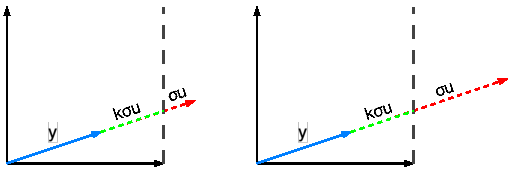
\includegraphics[width=\textwidth]{images/conflicting-workload.pdf}
    \caption{Visualisations of a Node's resource usage $y$ and expected resource
    usage $\sigma_1 u_1$ when learning of conflicting resource utilisation.}
    \label{fig:conflicting-workload}
\end{figure}

Figure \ref{fig:conflicting-workload} presents the scenario where a Node updates
its local model, learning that the experienced workload has increased in
resource usage ($\sigma_1$ has increased). This means that a smaller constant
$k$ is needed before the combined vectors cross a resource boundary. The Node,
thus, advertises a smaller capacity signal as it has less capacity for
the expected resource usage.

\begin{figure}[ht]
    \centering
    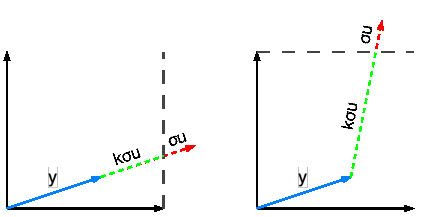
\includegraphics[width=0.8\textwidth]{images/complementary-workload.pdf}
    \caption{Visualisations of a Node's resource usage $y$ and expected resource
    usage $\sigma_1 u_1$ when learning of complementary resource utilisation.}
    \label{fig:complementary-workload}
\end{figure}

Figure \ref{fig:complementary-workload} presents the scenario where a Node updates
its local model, learning that the learned workload is using more resources but
in a different direction. This could be described as a complementary workload as
the the new expected resource utilisation requires a larger constant $k$ to
cross a resource boundary. Therefore, the Node advertises a higher capacity
signal as it has more capacity for the new expected resource utilisation.

\section{Reserve Cost and Capacity}
\label{sec:spazio-cost-capacity}
Like \textsc{Pronto}, \textsc{Carico}'s signal uses its current resource usage, and therefore, only
reflects Pods that have been scheduled and are running on the Node. For
\textsc{Carico} to account for Pod startup latency, the central scheduler must be able
to predict the a Pod's effect on a Node's signal. Consequently, \textsc{Carico}
assumes that Nodes know the number of currently running Pods and have the
ability to estimate their:
\begin{enumerate}
    \item \textbf{Baseline Capacity Signal:} the Capacity signal when no Pods
        are running
    \item \textbf{Per-Pod-Cost:} the estimated drop in Capacity signal will drop
        when a single Pod starts running.
\end{enumerate}
Section \ref{sec:estimating-cost} implements and compares different prediction
methods. With this information, a Node can calculate its Pod-Capacity (Capacity
given in units of Pods) from:
\begin{align}
    \text{Pod-Capacity} &= \frac{\text{Current Capacity Signal}}{\text{Per-Pod-Cost}} \\
    \text{Pod-Capacity} &= \frac{\text{Baseline Capacity Signal}}{\text{Per-Pod-Cost}}
    - \text{Current Pod Count}
\end{align}
This metric has two useful properties:
\begin{itemize}
    \item \textbf{Dual-Mode:} Pod-Capacity can be calculated
        using two equations. This is especially useful in Kubernetes as
        container creation and deletion can cause significant resource spikes,
        even with filtering in Figure \ref{fig:filtered-metrics-eval}, impacting
        immediate predictions.
        To combat this noise, Nodes can switch to predicting Pod-Capacity from
        previous Baseline and Per-Pod-Cost estimates. This reduces fluctuations
        in a Node's advertised Pod-Capacity and improves scheduling decisions
    \item \textbf{Unit of Measure:} As its unit of measure is in terms
        the number of Pods, it simplifies the central scheduler's logic,
        removing the need to keep track of each Node's Per-Pod-Cost.
\end{itemize}

\section{Central Scheduler}
Each Node $n$ will broadcast its $\text{Pod-Capacity}_n$ to a central scheduler. This
scheduler also tracks each Node's reserved amount as $\text{\# Pods Reserved}_n$. For
each Pending Pod, the scheduler performs the following operations:
\begin{itemize}
    \item \textbf{Filter:} Filters out all Nodes $n$ with $\text{Pod-Capacity}_n -
        \text{\# Pods Reserved}_n < 1$. Thus, the scheduler only considers Nodes
        with enough resources for another Pod. While reducing the threshold
        could pack more Pods on a Node, overallocation could result in OOM kills
        if there isn't enough memory available on a Node for all the Pods.
    \item \textbf{Score:} Score Nodes $n$ by $\text{Pod-Capacity}_n - \text{\#
        Pods Reserved}_n$. This ensures we allocate to Nodes which can fit more
        Pods.
    \item \textbf{Reserve:} Once a Node $n$ has been chosen, we increment
        $\text{\# Pods Reserved}_n$ by $1$. Once a scheduled Pod
        is no longer in the Pending state, the central scheduler decrements
        $\text{\# Pods Reserved}_n$ by $1$ for the Node $n$ the Pod was assigned
        to.
\end{itemize}

\section{Properties}
\textsc{Pronto} is designed to be \textit{federated, streaming} and
\textit{unsupervised}. \textsc{Carico} exhibits identical properties while also
considering the existence of communication and Pod start-up latency.

\textbf{Federated:}
While \textsc{Carico} uses a central scheduler to score Nodes and perform the final
Bind operation, it can still be considered federated because of its use
of FSVD: individual Nodes have a unified view of the global workload
while maintaining their individual autonomy to set their own score.

\textbf{Streaming:} Like \textsc{Pronto}, \textsc{Carico} only requires a single
pass over the incoming data in order to update its estimates. In addition,
Incremental-SVD only requires memory linear to the number of features
considered; given batches of dimension $d \times b$, the required memory is
proportional to $\mathcal{O}(d)$. This memory footprint can be further reduced
with low-rank approximation.

\textbf{Unsupervised:} \textsc{Carico} uses FSVD and assumptions about the
collected telemetry to generate values with capacity-based interpretations.
While this greatly differs from \textsc{Pronto} and its use of FPCA,
\textsc{Carico} still exploits the resulting subspace estimate along with the
incoming data to reveal patterns in recent resource-usage.

\textbf{Comparable:} \textsc{Pronto} is a binary signal, which makes it
difficult to score Nodes. \textsc{Carico}'s $\text{Pod-Capacity} \in
\mathbb{R}$, allowing Nodes to be filtered and scored against each other.

\textbf{Latency Resilient:} Unlike \textsc{Pronto} which assumes no communication
latency, \textsc{Carico} was designed with Kubernetes in mind, and thus must consider
possible latency in communication and Pod startup. \textsc{Carico}'s
$\text{Pod-Capacity}$'s unit of measure allows the central scheduler to easily
track the estimated cost of Pods in-flight, ensuring subsequent scheduling
decisions do not mistakenly overload a Node with a high $\text{Pod-Capacity}$.
%
% There are several methods to integrating the reserve cost into the signal to be
% sent to the central scheduler. The first method involves sending the signal and
% the reserve cost as separate values. On pod bind, we reserve the latest pod cost
% from the signal, and only relinquish the reserved amount once the central
% scheduler \verb|kube-apiserver| listener detects the pod is no longer Pending.
% This method requires the central scheduler to keep track of both the pods on
% each node and the pod-cost when the pod was bound.
%
% I instead chose to integrate the reserve quantity directly into the signal: each
% node calculates its available capacity in terms of no. of pods using two equations:
% \[ \text{avail. capacity from signal} = \frac{\text{signal}}{\text{per-pod-cost}} \\
   % \text{avail. capacity from no. of pods} = \frac{\text{capacity}}{\text{per-pod-cost}} -
   % \text{no. of pods} \]
%
% We use to functions for different situations. Typically, we calculate the
% available capacity from the latest signal measurements. However, if we detect a
% recent container event, the remote \verb|pronto| pod calculates the capacity
% from the pod count. This is to reduce the instability introduced by the
% container runtime. Furthermore, with this signal, the central scheduler does not
% have to record the per-pod-cost at bind time as the signal is now given in terms
% of individual pod counts. This simplifies the central scheduler and reduces the
% memory demand on.
%

\section{Related Work}
This section briefly identifies how \textsc{Carico} fits into the current
landscape of Kubernetes schedulers.

\subsection{Federated and Distributed Scheduling}
\textsc{Pronto} is described as a federated algorithm that executes plans in a
decentralised fashion. Each computing node makes independent decisions for task
assignments without needing global synchronisation. Custom Kubernetes schedulers
have been designed to extend the Kubernetes architectures with modular,
two-level, or distributed architectures \cite{beltre2019kubesphere, casquero2019distributed, luong2019multi, zhang2019multi}. However, the new
federated scheduler returns to a centralised architecture, mirroring the default
Kubernetes scheduler (\texttt{kube-scheduler}) with a single dispatcher on the
master node and has access to a global view of the Nodes.

\subsection{Performance-Aware and Predictive Scheduling}
As a performance-aware scheduler, \textsc{Carico} employs
dimensionality-reduction technique to efficiently process the vast amount of
telemetry data produced by each Node, with the goal of predicting a Node's
capacity for incoming workloads. While, CPU and RAM utilisation are common
metrics for performance-aware Kubernetes schedulers~\cite{bao2019deep,
beltre2019kubesphere, bestari2020dynamic, carvalho2021qoe, toka2021ultra},
\textsc{Carico} distinguishes itself with its ability to work with any metric
that can be [0,1]-normalised such that 0 indicates full capacity available and 1
indicates no capacity remaining.

Furthermore, the dynamic nature of Kubernetes workloads strongly suggest that
predictive techniques could improve scheduling efficiency and resource
utilisation, and still remains an open research
topic~\cite{carrion2022kubernetes}.

\subsection{Machine Learning-Based Schedulers}
Machine Learning (ML) algorithms  are increasingly adopted in scheduling to
learn from data and improving decision quality. These range from
Deep-Reinforcement learning-based schedulers \cite{bao2019deep, huang2020rlsk,
peng2021dl2, han2021tailored} that use reward functions to continuously improve
scheduling decisions, to domain-specifc to application or resource utilisation
predictions~\cite{yang2019design, carvalho2021qoe, harichane2020proposal}.
Instead, \textsc{Carico} exploits properties of simple SVD to learn
characteristics of recent workloads, giving it broad applications with minimal
complexity.

\subsection{Summary of Related Work}
In summary, \textsc{Carico} distinguishes itself within the Kubernetes
scheduling landscape through its combined federated and centralised nature, and
use of FSVD to predict a Node's capacity for incoming workloads.


\chapter{Implementation}

\section{System Architecture}
\label{sec:sys-arch}

\begin{figure}[ht]
    \centering
    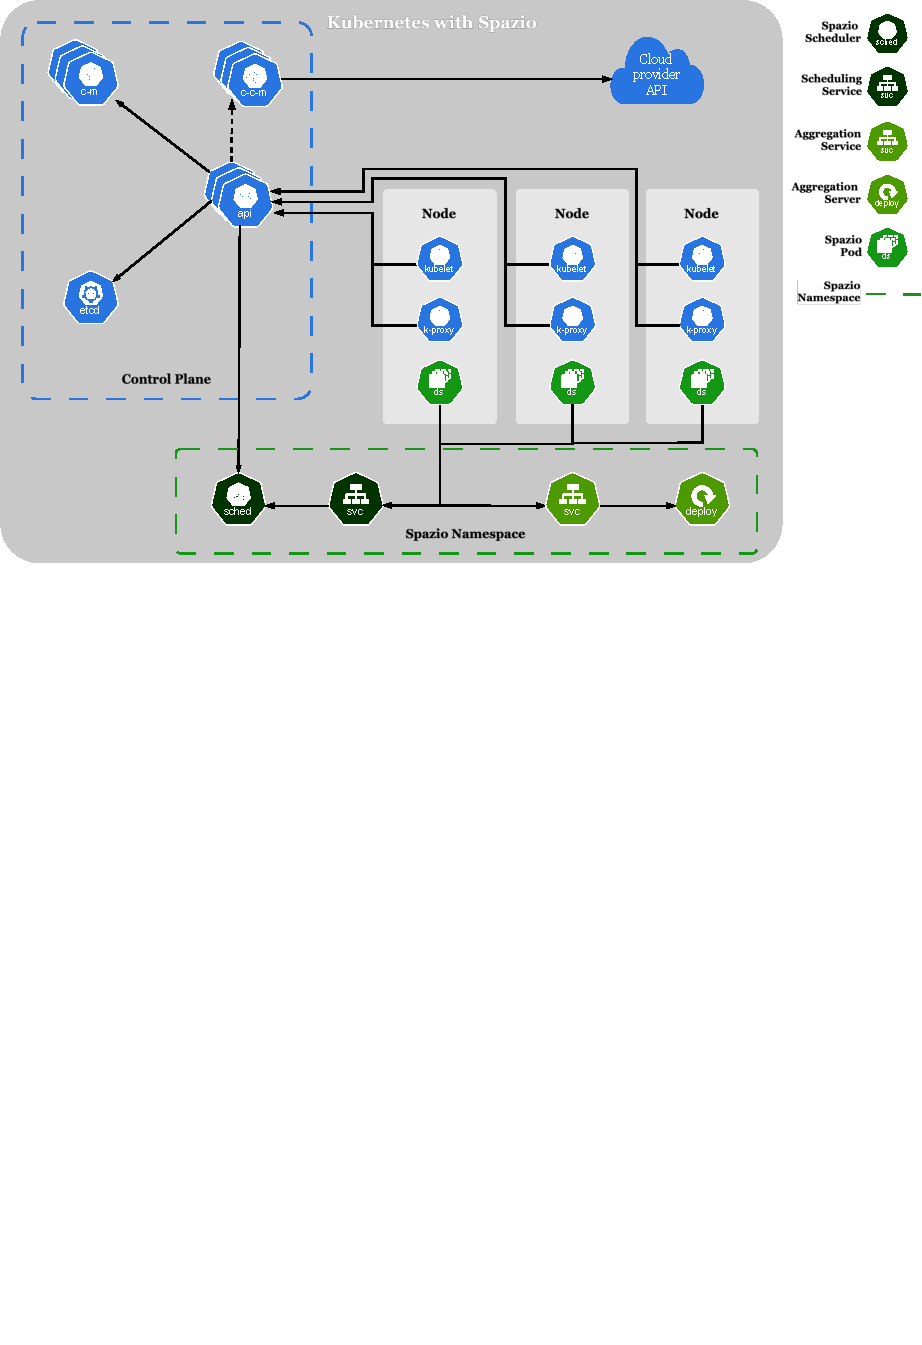
\includegraphics[width=\textwidth]{images/carico-svg.pdf}
    \caption{The components within the \textsc{Carico} system}
    \label{fig:spazio-system}
\end{figure}

The \textsc{Carico} system consists of three core components (shown in figure
\ref{fig:spazio-system}):
\begin{itemize}
    \item \textsc{Carico} DaemonSet: each Node in the cluster will contain a \textsc{Carico} Pod.
        This Pod periodically collects telemetry from the Node and generates its
        local model and a capacity signal, which it sends to the Scheduling
        Service. When the \textsc{Carico} Pod deems its local model outdated, it requests
        the latest aggregated global model from the Aggregation service.
    \item Aggregation Server: This deployment provides the Aggregation service.
        The Aggregation Server Pod receives local models from Nodes
        and returns the latest aggregated global model.
    \item Scheduler: In \textsc{Carico}, the scheduler is a \textbf{Scheduler Plugin},
        implementing custom Filter, Score and Reserve functions. It also acts as
        the server of the Scheduling service, receiving the latest capacity
        scores of each Node to inform its scheduling decisions.
\end{itemize}

\section{\textsc{Carico} Pod}
\begin{figure}[H]
    \centering
    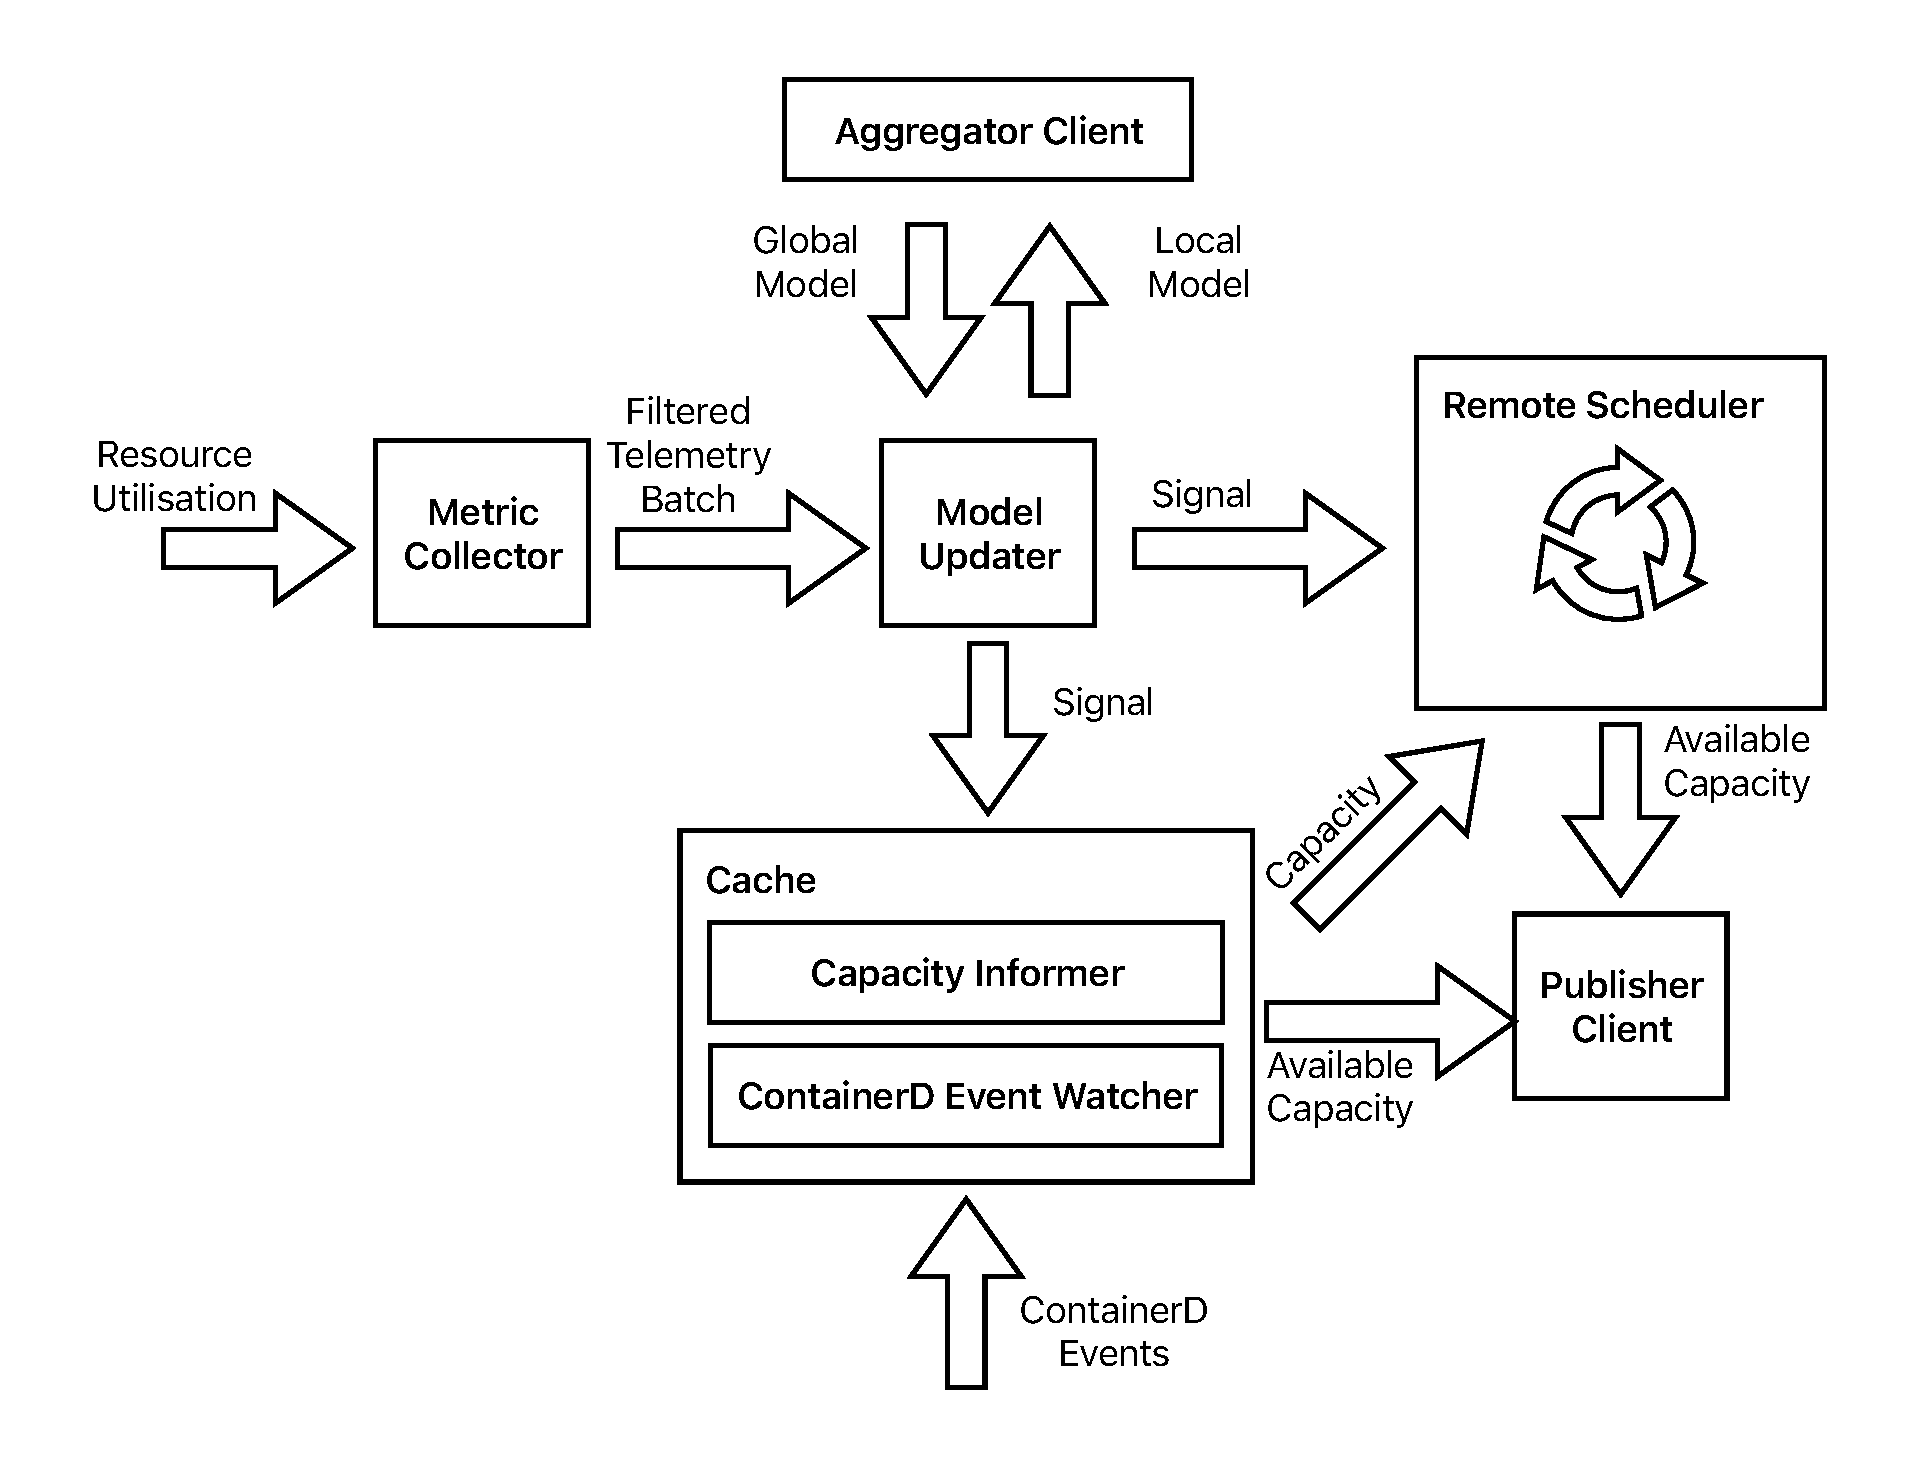
\includegraphics[width=\textwidth]{images/spazio-pod.pdf}
    \caption{Core components within the \textsc{Carico} Pod}
    \label{spazio-pod-components}
\end{figure}
As mentioned in section \ref{sec:sys-arch}, the \textsc{Carico} Pods are defined within a
DaemonSet - a DaemonSet ensures that all Nodes run a copy of a Pod. The \textsc{Carico}
Pods collect telemetry from the Node and generate its local model and capacity
signal. The following sections detail the metrics considered and explain the
corresponding implementation decisions.

\subsection{Metric Collection}
To build its local model, the \textsc{Carico} Pod must first collect telemetry.
Kubernetes offers numerous ways to obtain telemetry data. I explored two primary
sources of telemetry data:
\begin{itemize}
    \item Metrics Server: a cluster add-on that acts as a centralised source of
        container reosurce metrics.
    \item \verb|/proc/|: a pseudo-filesystem within Linux that exposes real-time
        information about running processes and system's hardware.
\end{itemize}

With Metrics Server, a scraper is used to periodically (default every 15
seconds) collects resource metrics from Kubelets and exposes them from its
\verb|metrics.k8s.io/v1| APIService. While simple to use, it offers limited
metrics (CPU and RAM utilisation only) and introduces additional latency.
Moreover, its default 15 seconds scraping interval is too infrequent,
potentially missing short-lived Pods entirely.

\verb|/proc/|, conversely, offers low latency access to an up-to-date view
of the current state of the system. Furthermore, \verb|/proc/| contains various
files and subdirectories, each providing specific information. Examples include,
\verb|/proc/stat| which contains the amount of time CPU cores spend in different
states, \verb|/proc/meminfo| provides statistics about memory usage,
\verb|/proc/diskstats| presents the raw, low-level I/O statistics of all block
devices. Finally, both these sources are not generated periodically, but rather
on-the-fly. This guarantees that the information you see is as current as the
system's internal state.

Given these advantages, I selected \verb|/proc/| as the source of telemetry
data. The subsequent sections detail the metrics I considered and their
rationale behind their use.

% I decided to collect CPU and memory utilisation as my telemetry data, as these
% metrics are easily accessible and are used in a variety of industry-standard
% schedulers
 % In addition, it would take $15 \times \text{batch size}$
% seconds between model updates (required to collect a single
% batch before performing subspace merging), and would result in a less
% representative and out-of-date model of "current" resource usage.

\subsubsection{Utilisation Metrics}
\texttt{/proc/} can generate standard utilisation metrics (e.g., CPU and memory
percentage usage). These metrics are widely used in
industry~\cite{hadoop2016apache,sahasrabudhe_improved_2015}.

To collect CPU utilisation, I used the \verb|/proc/stat| file. This file reports
the cumulative count of "jiffies" (typically hundredths of a second) each CPU
spent in a specific mode \cite{proc_stat5}. I can then calculate CPU utilisation
using:
\[ \text{CPU Usage\%} = 1 - \frac{\Delta\text{idle} +
\Delta\text{iowait}}{\Delta\text{across all fields}} \]
\verb|/proc/meminfo| can also be used to collect memory utilisations. This file
shows a snapshot of the memory usage in kilobytes. The percentage of memory
used can then be calculated from the given field:
\[ \text{Memory Used\%} = 1 - \frac{\text{MemFree} +
\text{Buffers} + \text{Cached}}{\text{MemTotal}}\]

\begin{figure}[H]
    \centering
    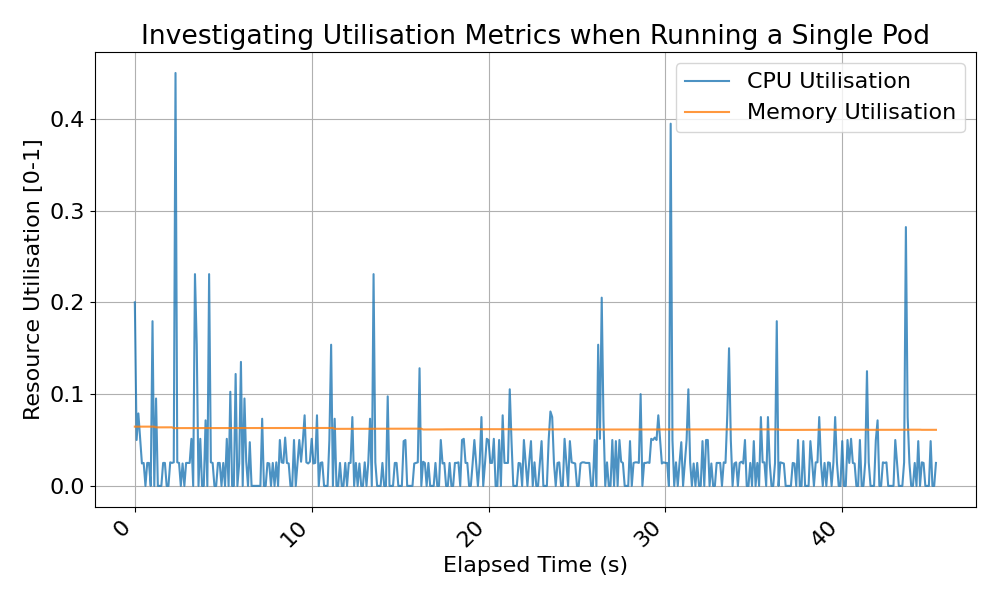
\includegraphics[width=0.45\textwidth]{images/utilisation-baseline.png}
    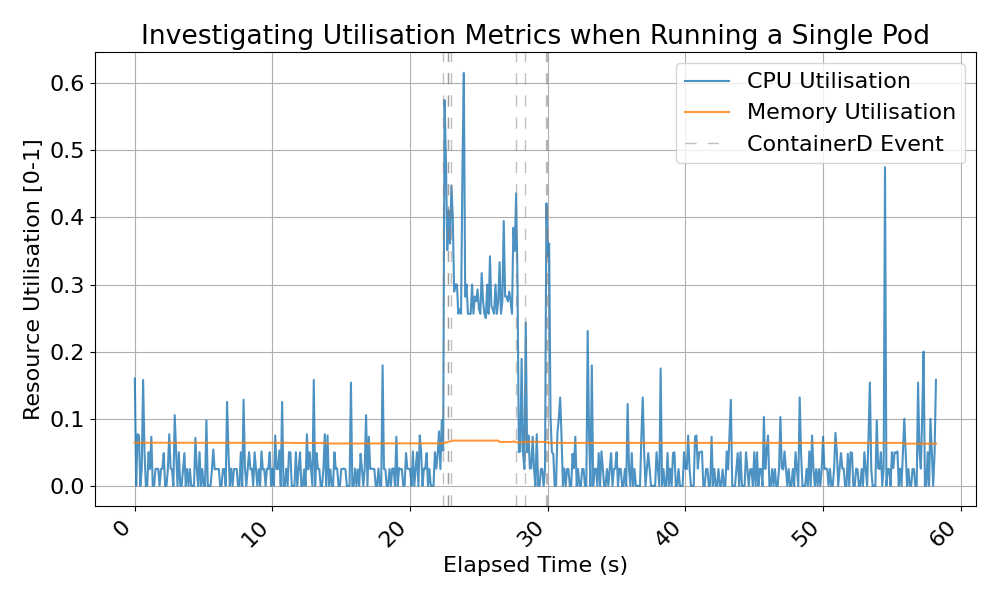
\includegraphics[width=0.45\textwidth]{images/utilisation-single.png} \\
    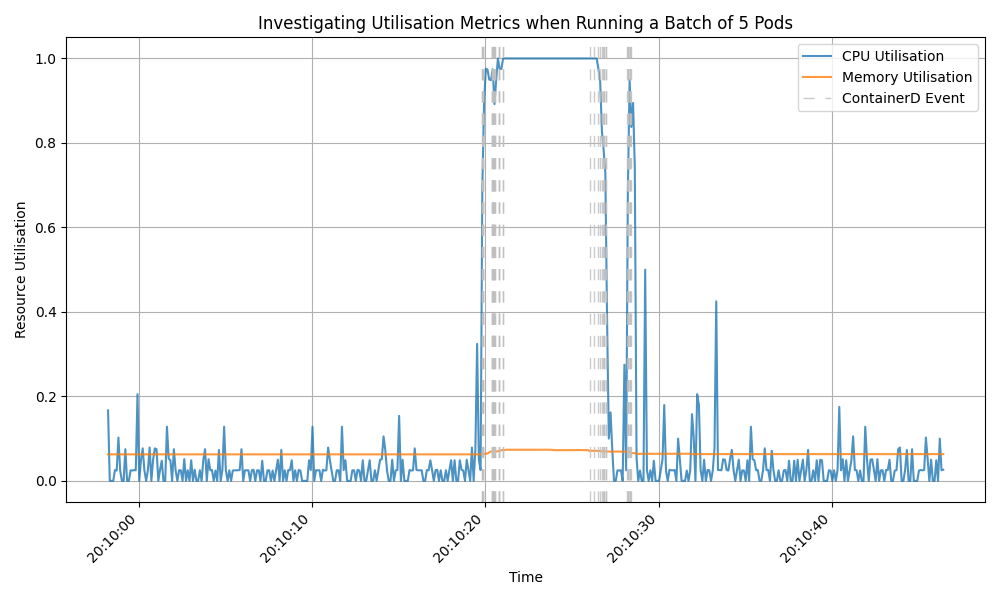
\includegraphics[width=0.45\textwidth]{images/utilisation-smallbatch.png}
    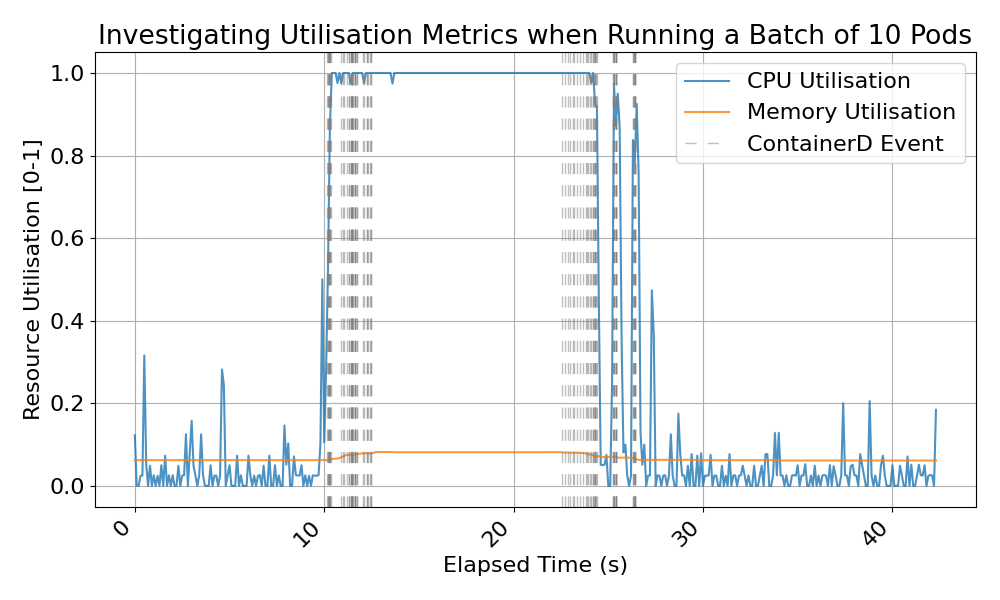
\includegraphics[width=0.45\textwidth]{images/utilisation-bigbatch.png}
    \caption{In this figure we sample CPU and memory utilisation from
    values of \texttt{/proc/stat}, \texttt{/proc/meminfo} at 10Hz during various
    Kubernetes workloads.}
    \label{fig:utilisation-eval}
\end{figure}

To assess their suitability for \textsc{Carico}, I measured utilisation metrics
under various workloads. Figure \ref{fig:utilisation-eval} presents the metrics
behaviour when running different Job sizes of \verb|pi-2000| Pods. For a
CPU-intense workload (calculating $\pi$ to 2000 digits), the CPU utilisation
correctly increased while memory utilisation remained stable.

\subsubsection{Issues of using CPU Utilisation}
\label{sec:issue-with-util}
Early prototypes using only utilisation metrics showed poor throughput compared
to the default \verb|kube-scheduler|, highlighting a problem with relying solely
on CPU utilisation. When deploying 1000 Pods, each requesting 100 milliseconds
of CPU time, across 19 Nodes, the \verb|kube-scheduler| would immediately
allocate all Pods evenly across the Nodes. This would result in $\approx$ 45
Pods running on each Node. In contrast, \textsc{Carico} (using only utilisation
telemetry) allocated at most 5 Pods concurrently per Node. In both situations,
CPU utilisation was 100\%, however, the default \verb|kube-scheduler| managed to
achieve a high throughput, even with a long-tailed distribution of individual
Pod completion times.

\begin{figure}[H]
    \centering
    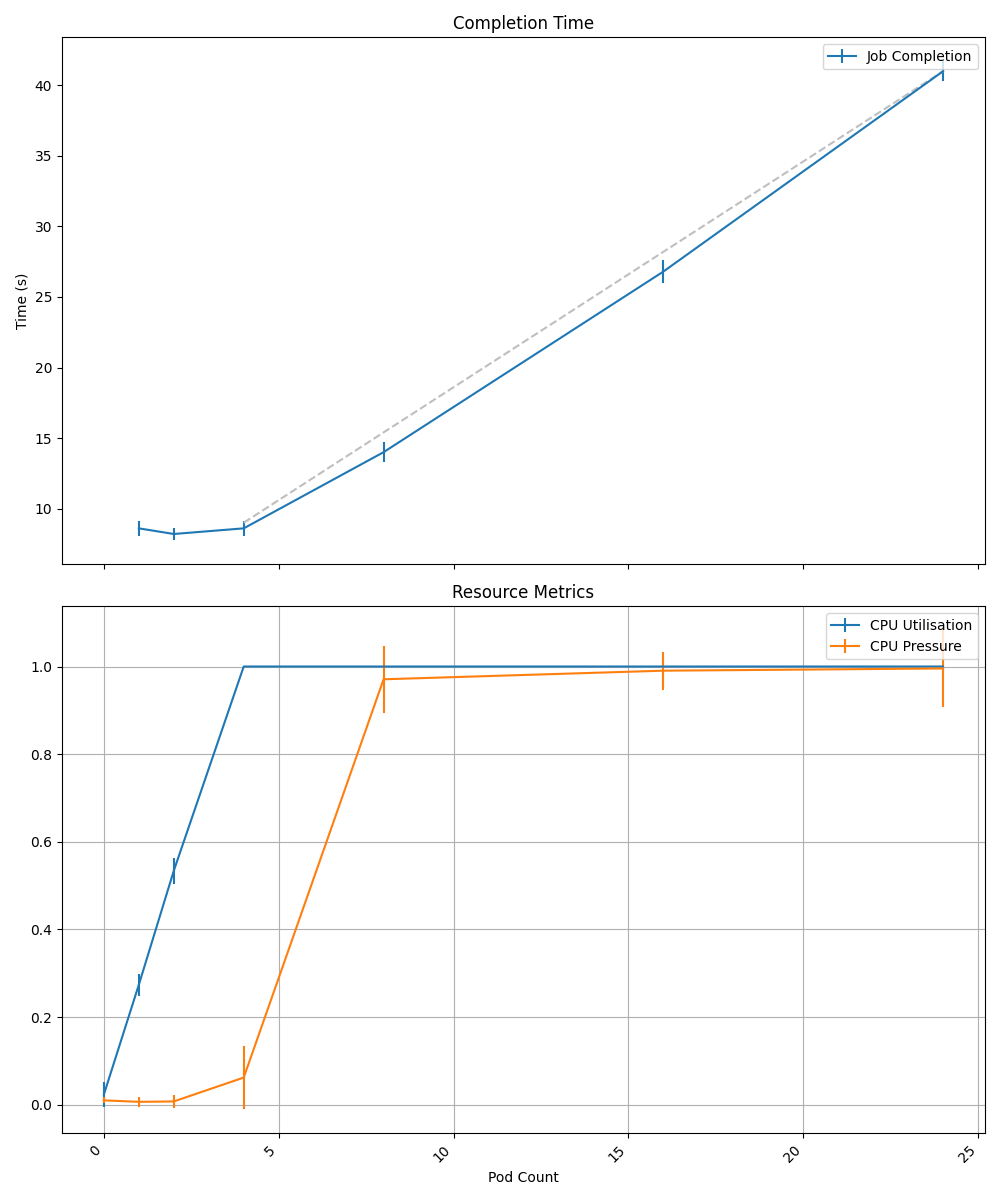
\includegraphics[width=0.45\textwidth]{images/podcount-util-pressure.png}
    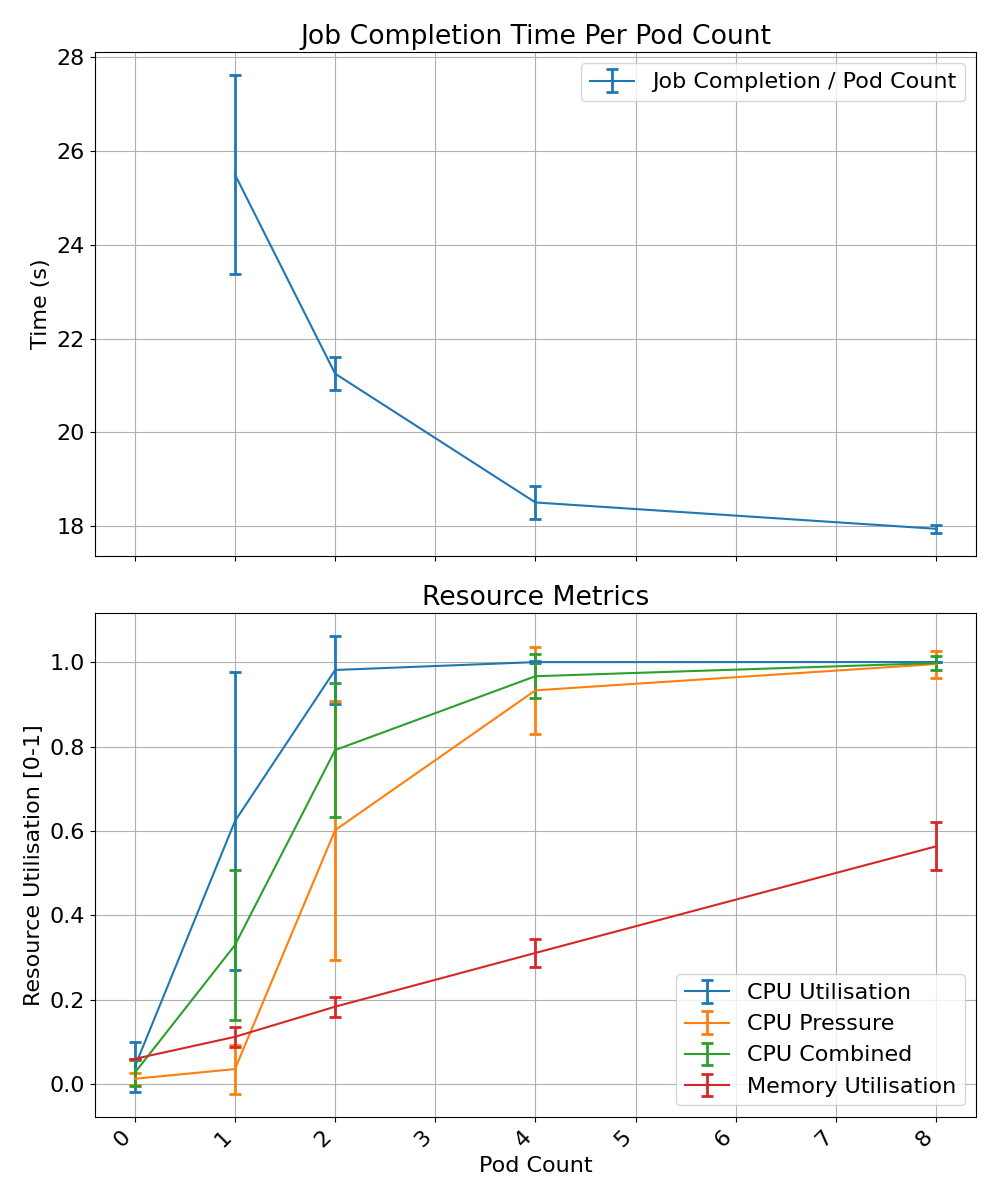
\includegraphics[width=0.45\textwidth]{images/ml-podcount-util-pressure.png}
    \caption{Collected resource metrics during various Kubernetes workload.}
    \label{fig:podcount-util-pressure}
\end{figure}

As a result, I decided to further investigate this phenomenon. Figure
\ref{fig:podcount-util-pressure} shows how a Job's completion time changes as you
increase its completion and parallelism count when running different Pods:
cpu-intense Pi-2000 and a small ML workload (training and inference). I also
decided to include measurements from \verb|/proc/pressure|. This investigation
revealed that the relationship between the number of Pods running on
a Node at a time and their completion time showed a close-to linear
relationship. I hypothesise that this is because the cluster runs on virtual
machines (VMs). Hypervisors, while abstracting hardware, can mask effects like
cache contention and CPU thrashing. This means that high  CPU utilisation may
not truly signify performance degradation. Thus, CPU utilisation alone is not a
definitive capacity measure, explaining the prototype's initial throughput
limitations.

\subsubsection{Combining CPU Utilisation and CPU Pressure}
Raw \verb|/proc/pressure| metrics were also insuffice as these metrics
barely increased until the Pod count exceeded core count. This would lead to
unreasonably low intial Per-Pod-Cost estimations and an inflated advertised Node
Pod-Capacity. I therefore combined both CPU utilisation and CPU pressure
into a single metric:
\[ CPU = \frac{\text{CPU Utilisation} + \text{CPU Pressure}}{2} \]

This ensures the metric increases with Pod count but doesn't saturate to
quickly. This combined CPU metric only reaches its maximum when \verb|/proc/pressure|
indicates persistant CPU demand (at least one thread always waiting). Figure
\ref{fig:podcount-util-pressure} illustrates this metric in action.

\subsection{Filtering Metrics}
\textsc{Carico} does not perform peak detection, but its signal is still
susceptible to short-lived spikes. As previously noted,  Pod creation and
deletion incur visible resource usage spikes. These spikes introduce noise
into both the Node's local model, as well as, its Capacity signal. A noisy
signal complicates baseline Capacity and Per-Pod-Cost estimation. As such, I
needed to de-noise the original metrics.

Investigation into the recorded telemetry showed that the spikes caused from
container events would last $\approx$200 milliseconds. Sampling at
10Hz, Dynamic EMA was used to suppress container-event caused spikes (typically
$\approx$ 200ms) while allowing rapid convergence for sustained changes (spikes
$>$ 300ms).

\begin{figure}[H]
    \centering
    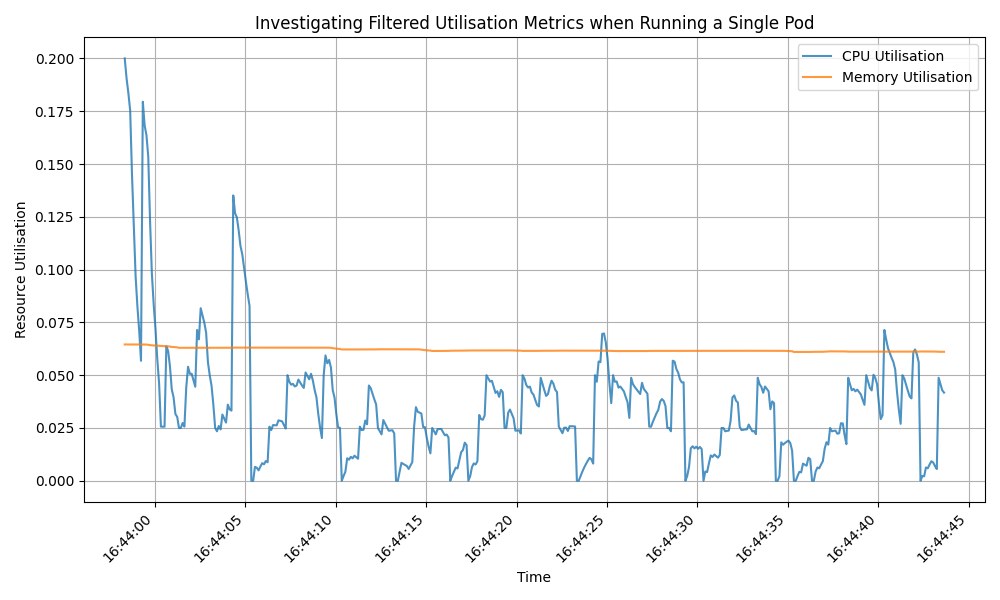
\includegraphics[width=0.45\textwidth]{images/filter-utilisation-baseline.png}
    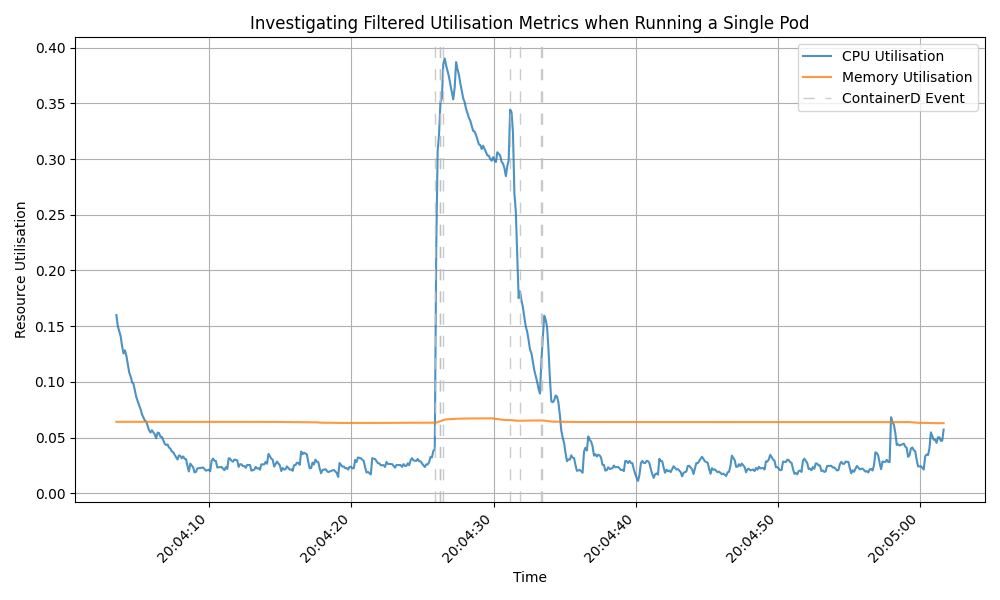
\includegraphics[width=0.45\textwidth]{images/filter-utilisation-single.png} \\
    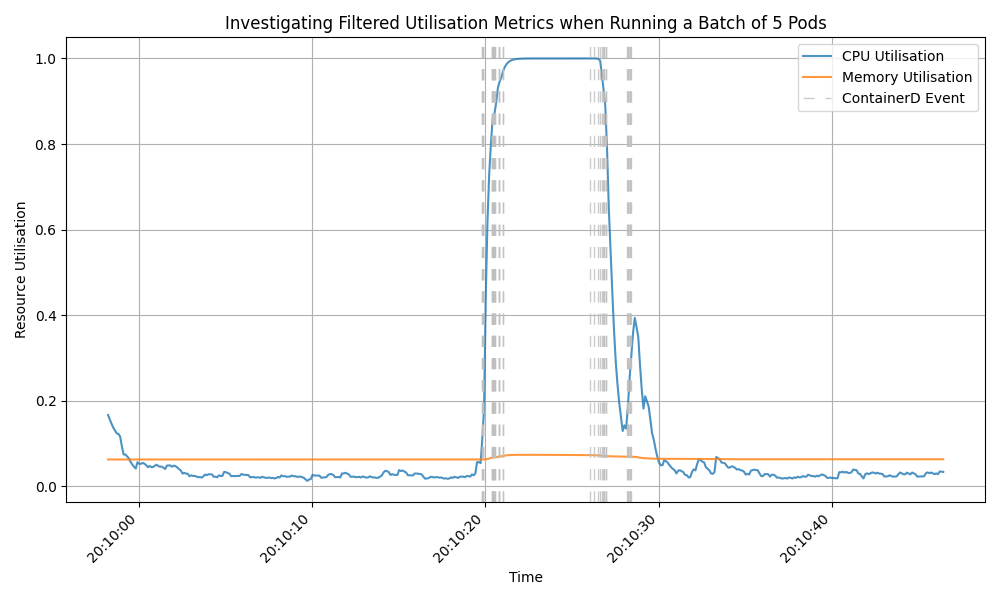
\includegraphics[width=0.45\textwidth]{images/filter-utilisation-smallbatch.png}
    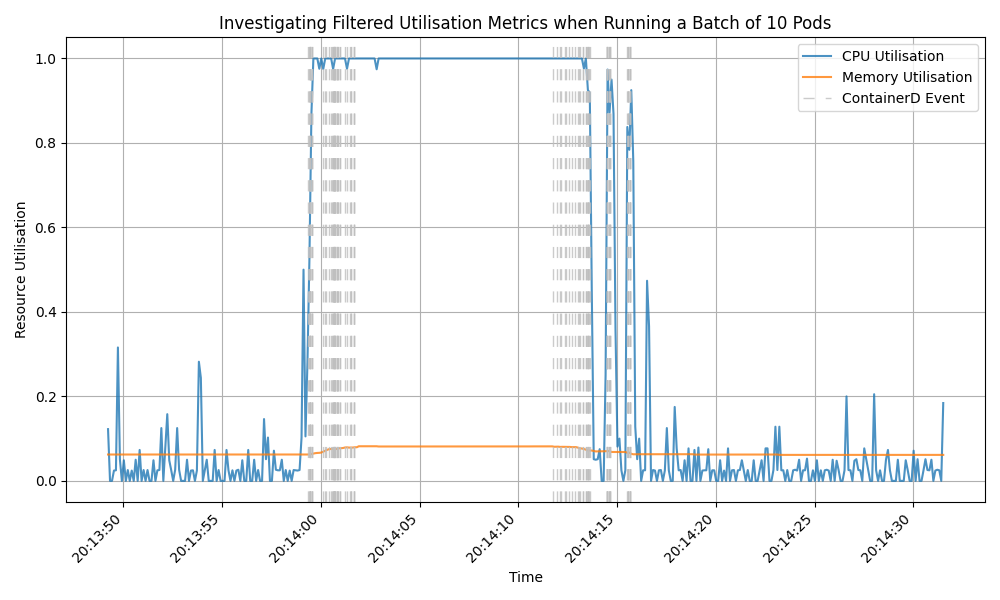
\includegraphics[width=0.45\textwidth]{images/filter-utilisation-bigbatch.png}
    \caption{This figure shows the smoothed metrics under different workloads.}
    \label{fig:filtered-metrics-eval}
\end{figure}

Comparing Figure \ref{fig:utilisation-eval} with \ref{fig:filtered-metrics-eval}
demonstrates the dampening of the Dynamic EMA and its quick responsive to
prolonged changes in workloads. More sophisticated filters were avoided due to
their higher computational cost, which would rob resources from scheduled Pods.
Filtering the signal directly, rather than the telemetry, was considered but
rejected as it would still allow container-event resource spikes to pollute the
local model.

\subsection{Signal Generation}
The \textsc{Carico} Pod calculates its Capacity signal at 1Hz. This matches the local
model update frequency, ensuring that the Capacity signal tracks with the local
model. While a higher frequency would provide the central scheduler a more
current view of a Node's resource status, it would also increase resource
overhead. This overhead would reduce the available resources to other
Pods and could also lower the baseline Capacity signal, potentially reducing
the capacity a Node advertises.

To verify Capacity signal's implementation, I tested it under the scenarios
described in Section \ref{sec:signal-example-scenario}. For the conflicting
workload, I had the measured Node execute a light CPU-focused workload
(\texttt{ng-stress --cpu=8 --cpu-load=25}) with the surrounding Nodes executing
a CPU-intense workload (\texttt{bpi(2000)}). For the complementary workload, the
measured Node executed a light Memory-focused workload (\texttt{ng-stress --vm=4
--vm-bytes=4G}) with the surrounding Nodes also executing the same CPU-intense
workload as in the conflicting scenario. The measured signals are shown in
figures \ref{fig:signal-evaluation-cpu} and \ref{fig:signal-evaluation-mem}

\begin{figure}[H]
    \centering
    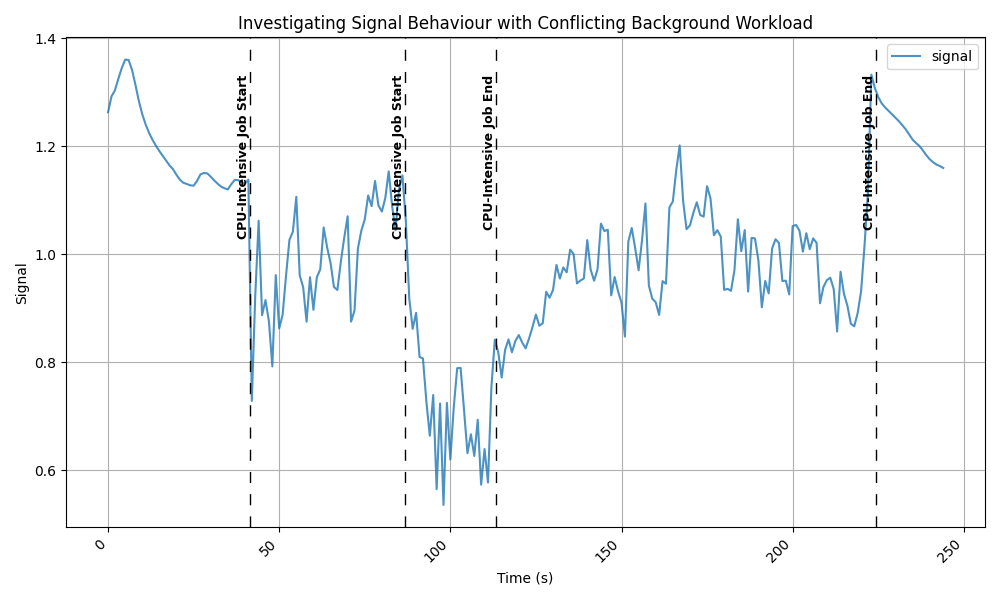
\includegraphics[width=\textwidth]{images/signal-with-cpu.png}
    \caption{The calculated capacity signal of a Node running \texttt{ng-stress
    --cpu=8 --cpu-load=25}. While running this workload, $1000$ Pods running
    \texttt{bpi(2000)} were scheduled across surrounding Nodes.}
    \label{fig:signal-evaluation-cpu}
\end{figure}
\begin{figure}[H]
    \centering
    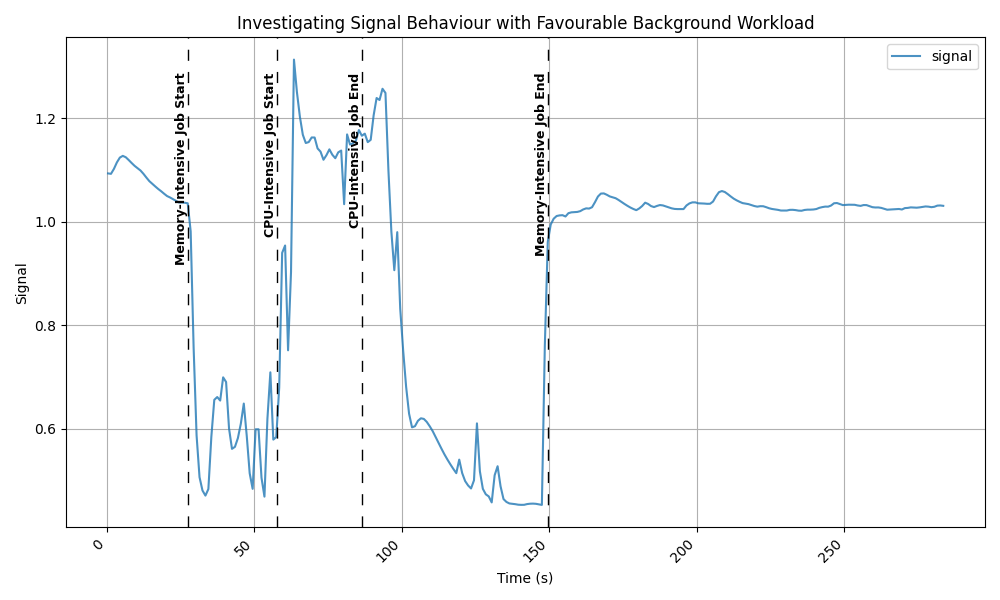
\includegraphics[width=\textwidth]{images/signal-with-memory.png}
    \caption{The calculated capacity signal of a Node running \texttt{ng-stress
    --vm=4 --vm-bytes=4G}. While running this workload, $1000$ Pods running
    \texttt{bpi(2000)} was scheduled across surrounding Nodes.}
    \label{fig:signal-evaluation-mem}
\end{figure}

Figures \ref{fig:signal-evaluation-cpu} and \ref{fig:signal-evaluation-mem}
demonstrates how a Node's capacity signal reacts to changes in surrounding
workloads when experiencing different resource usage. In Figure
\ref{fig:signal-evaluation-cpu}, the measured Node is running a light CPU-focused
workload. Once the CPU-intense workload is scheduled on surrounding Nodes, the
measured Node's capacity signal drops. This is expected as the local models of
surrounding Nodes will reflect a more costly CPU-focused workload. As a result,
when the measured Node aggregates its local model, its new model will reflect
this higher CPU usage with a larger $\sigma_1$ value. Since both the Node's
current resource usageand the learned expected workload (reflected in $u_1$) are
CPU-focused, the increased magnitude of the expected workload (larger
$\sigma_1$) results in a smaller $k$ (fewer units of this workload can be
added), and thus a lower Capacity signal.

In Figure \ref{fig:signal-evaluation-mem}, the measured Node runs a light
memory-focused workload. When the CPU-intense workload is scheduled on surrounding
Nodes, the measured Node's capacity signal increases. This aligns with the
hypothesis from Section \ref{sec:capacity-signal}. Like in the previous scenario, the global model
reflects a heavy CPU-focused workload, and thus, so will the aggregated local
model of the measured Node. However, with the Node's current resource usage
(memory-focused) now largely orthogonal to the learned expected workload
(CPU-focused), a larger $k$ is required to reach a resource limit.

\subsection{Calculating Cost and Capacity}
Since the \textsc{Carico} Capacity signal incorporates current resource usage,
newly scheduling (but not yet running) Pods do not immediately affect the
Capacity signal. Therefore, a signal reservation mechanism is needed to prevent
the scheduler from greedily overloading the Node with the current highest score.
To handle varying Pod workloads, a dynamic estimation of a Pod's "signal cost"
was required. The method also needed to handle concurrent Pod creation and
deletions.

\subsubsection{Detecting Pod Events}
\label{sec:listeners-comparison}
There are numerous ways to detect the addition and removal of Pods from a Node.
I investigated two event detection approaches: watching the Kubernetes API vs
ContainerD events. The goals of the listeners were as follows:
\begin{itemize}
    \item Detect the creation and deletion of Pods to establish a Pod count
    \item Provide warning for potential container-caused churn
\end{itemize}
This warning is crucial because the Dynamic EMA can't fully smooth prolonged
resource spikes from multiple, concurrent container events. Early detection
allows temporarily halting estimations during such bursts.
\begin{figure}[H]
    \centering
    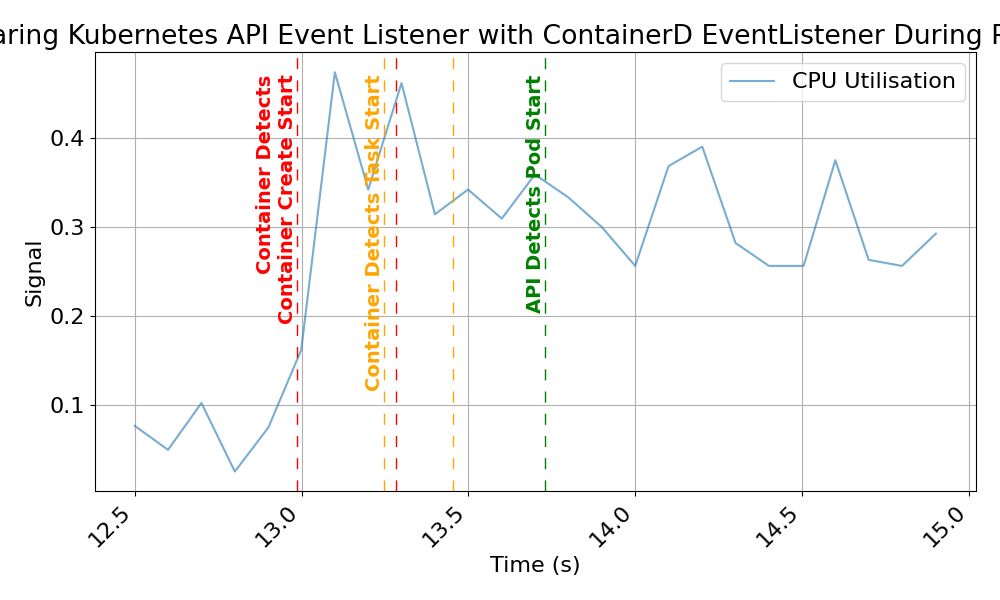
\includegraphics[width=\textwidth]{images/event-comparison-start.png}
    \caption{When different event listeners detected the creation of a Pod.}
    \label{fig:event-evaluation-start}
\end{figure}

\begin{figure}[H]
    \centering
    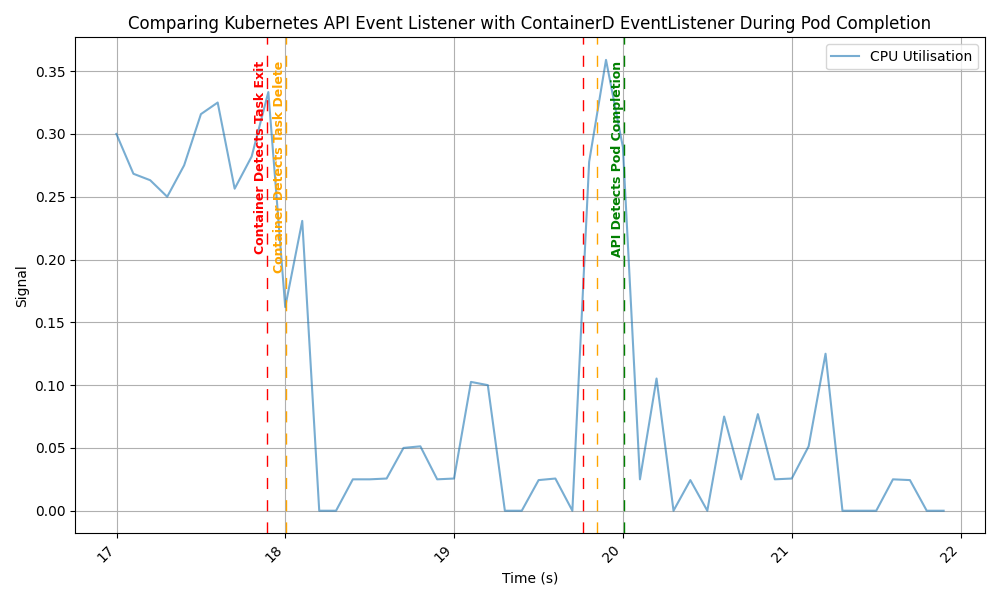
\includegraphics[width=\textwidth]{images/event-comparison-end.png}
    \caption{When different event listeners detected the completion of a Pod.}
    \label{fig:event-evaluation-end}
\end{figure}

Figures \ref{fig:event-evaluation-start} and
\ref{fig:event-evaluation-end} show that communication latency from the
Kubernetes API causes its listener to miss container runtime resource spikes.
Without forewarning, Nodes would incorporate these spikes into
their predictions. On the other hand, we can see that certain container
events precede the spikes. Though more complex, handling ContainerD events
directly provides earlier warnings, reducing noise in calculations.

\subsubsection{Estimating Pod-Cost}
\label{sec:estimating-cost}
To produce a \textbf{reservable} signal, as per Section
\ref{sec:spazio-cost-capacity}, \textsc{Carico} requires Nodes to estimate their
baseline Capacity and Per-Pod-Cost. has the capability of estimating its
capacity and per-Pod cost. I needed a streaming signal processing technique with
a low-overhead and the ability to work with a dynamic system (handle changes in
workloads over time). A Kalman filter \cite{} is a powerful algorithm used for
estimating the true state of a dynamic from a series of noisy and uncertain
measurements. It's widely applied in fields like navigation (GPS), robotics,
signal processing and control systems. Its ability to estimate a system's state
from noisy measurements makes it suitable for this dynamic environment.

I devised three Kalman filter-based approaches to estimating reservation costs.
\begin{itemize}
    \item 1D Kalman Filter predicting reservation cost based on the function:
        \[\Delta \text{signal} = \Delta \text{no. of running Pods} \times
        \text{cost}\]
    \item 2D Kalman Filter to predict the signal based on the function:
        \[\text{signal} = \text{capacity} + \text{per Pod cost} \times \text{no.
        of Pods}\]
    \item Two separate 1D Kalman Filters predicting the equation:
        \[\text{signal} = \text{capacity} + \text{per Pod cost} \times \text{no.
        of Pods}\]
        Here, each filter learns a separate variable. This separation prevents
        non-zero covariance entries in the state covariance matrix ($\mathbf{P}$),
        mitigating oscillations observed with a single 2D Kalman filter.
\end{itemize}
To smooth out predictions, I employed two techniques. First, upon detecting
container churn via the event listener, the \textsc{Carico} Pod temporarily
halts estimations. Second, estimations are halted if the Capacity signal reaches
zero. When the capacity signal is 0, it indicates that at least one resource is
at capacity. If this occurs and another Pod begins running on the same Node, the
signal still outputs 0. Otherwise, the filters might inaccurately decrease the
Per-Pod-Cost, leading to an inflated advertised capacity.

\begin{figure}[H]
    \centering
    % 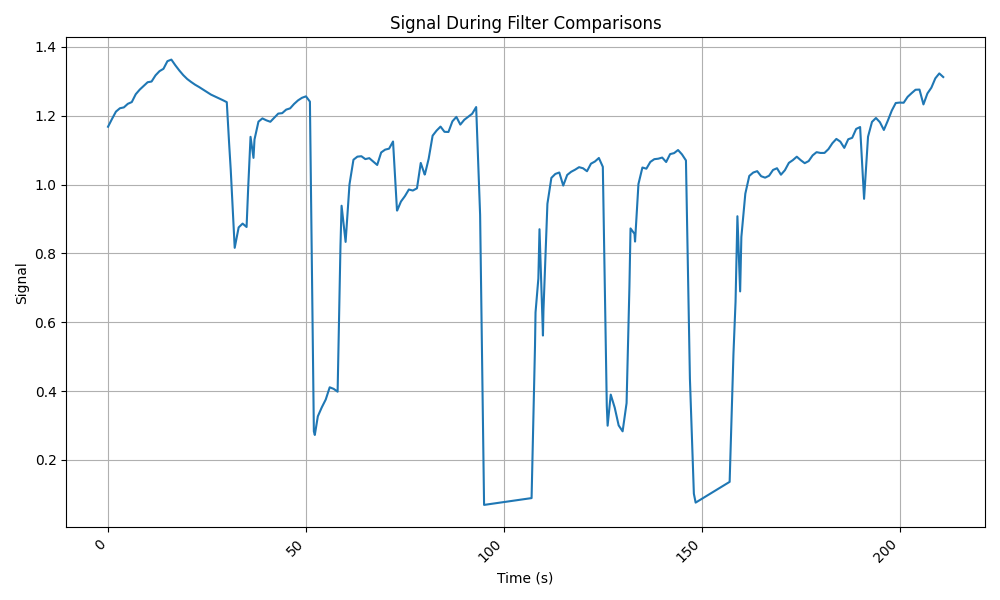
\includegraphics[width=0.45\textwidth]{images/filter-signal.png}
    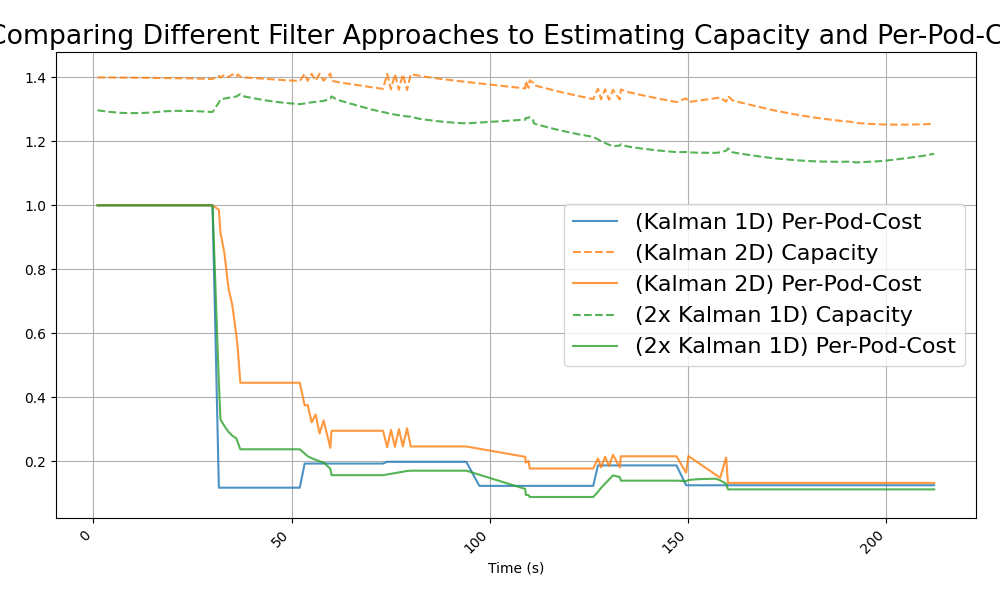
\includegraphics[width=\textwidth]{images/filter-comparison.png}
    \caption{The estimates of the Kalman filters when Node experiences
    variable-sized bursts of \texttt{bpi(2000)} Pods.}
    \label{fig:filter-evaluation}
\end{figure}
To decide the optimal approach, I observed each methods' behaviour when
executing Jobs of various sizes. This is depicted in Figure
\ref{fig:filter-evaluation}.
The $\Delta$-based Kalman filter accurately estimated Per-Pod-Cost, but being
one-dimensional, could not estimate the Node's baseline Capacity signal. The 2D
Kalman filter approach provides a simple method for estimating both the Node's
capacity and its per-Pod cost. Faster convergence for the 2D filter was
attempted using large process noise covariance ($\mathbf{Q}$) values. This, however,
led to large oscillations, as the filter adjusted both baseline capacity and
cost variables to correct errors. The dual 1D Kalman filter was inspired by the
stability of the 1D Kalman filter. This filter converged quickly and accurately
without exhibiting the oscillations that plagued the 2D Kalman filter.

\section{Aggregation Server}
\textsc{Pronto} aggregation resembles the distributed agglomerative summary
model (DASM) \cite{}. Local models are aggregated in a "bottom-up" approach
following a tree-structure depicted in Figure \ref{pronto-agg}. While this
approach reportedly requires minimal synchonisation, it demands
multiple dedicated Pods, and Kubernetes' inherent communication latency could
significantly delay global model updates after workload changes.

Therefore, I opted for a ``flat" on-the-fly aggregation approach: when the
Aggregation Server receives an aggregation request with a Node's local model,
instead of aggregating the local model and returning the new global model, the
server first enqueues the local model to be aggregated and returns its current
view of the global model. This implementation trades consistency for latency.

\begin{figure}[ht]
    \centering
    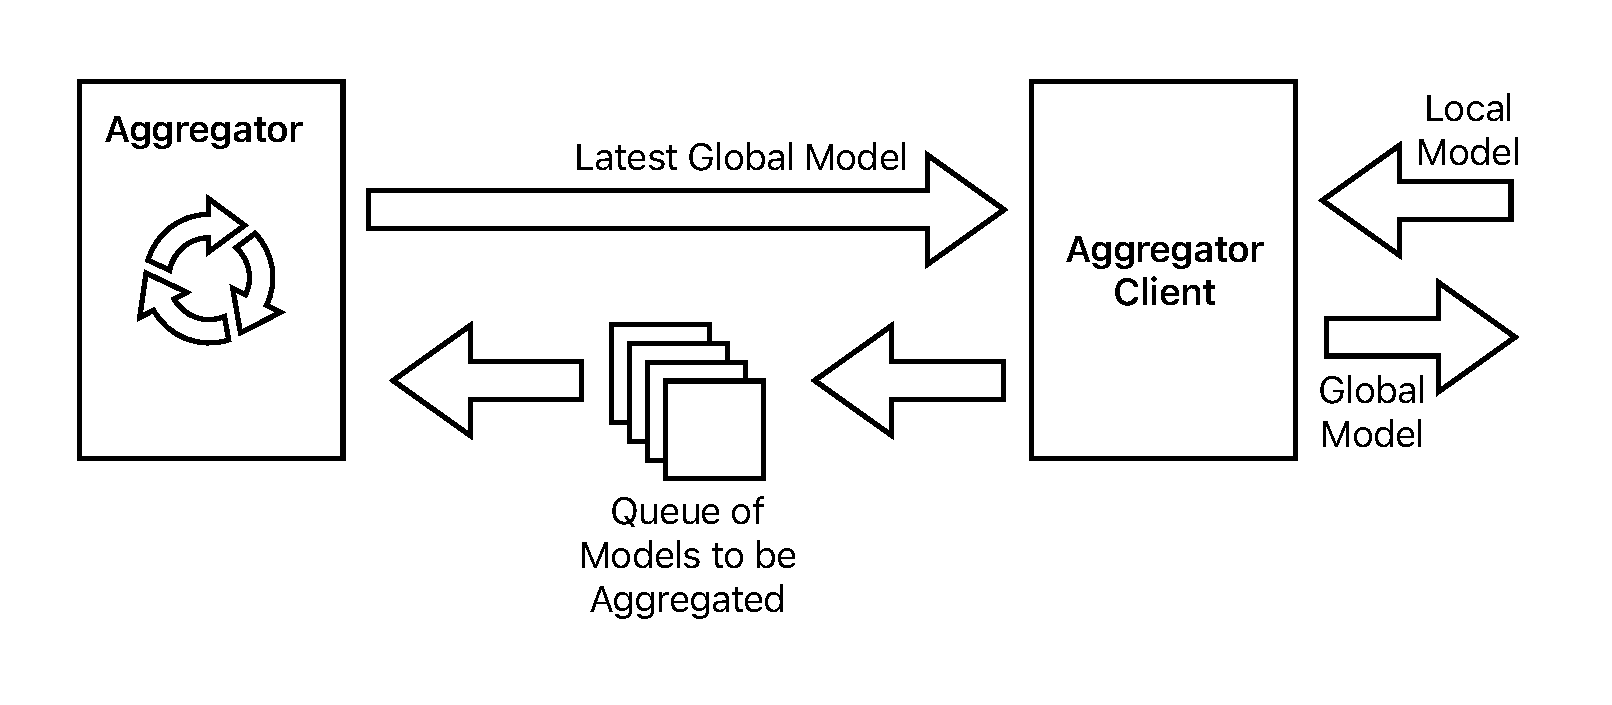
\includegraphics[width=\textwidth]{images/spazio-agg.pdf}
    \caption{The components within the Aggregator Server.}
    \label{spazio-agg-components}
\end{figure}

The Aggregation Server executes a thread which waits on a queue of local models
to aggregate. When the queue is non-empty, the thread pops the local model and
performs a Subspace Merge operation (as defined in \ref{sec:local-merge}). To
balance the influence of each local model, weights $\gamma_{\mathbf{A}} =
\text{\# of Nodes} - 1$ and $\gamma_{\mathbf{B}} = 1$ are used in the
Subspace-Merge (as per Section \ref{sec:local-merge}).
Aggregation clients perform a gRPC call to the address specified by the
Aggregation Service. This gRPC function is implemented by the server and takes
the local model of a Node as its argument. The function first enqueues the local
model to be merged and returns the latest view of the global model. Clients
then aggregate their own local model with the received global model. Decoupling
model aggregation from the gRPC call's critical path reduces server load,
improving its capacity to handle more clients.

\section{Scheduler Pod}
\subsection{Kubernetes Scheduler Plugin}
\begin{figure}[H]
    \centering
    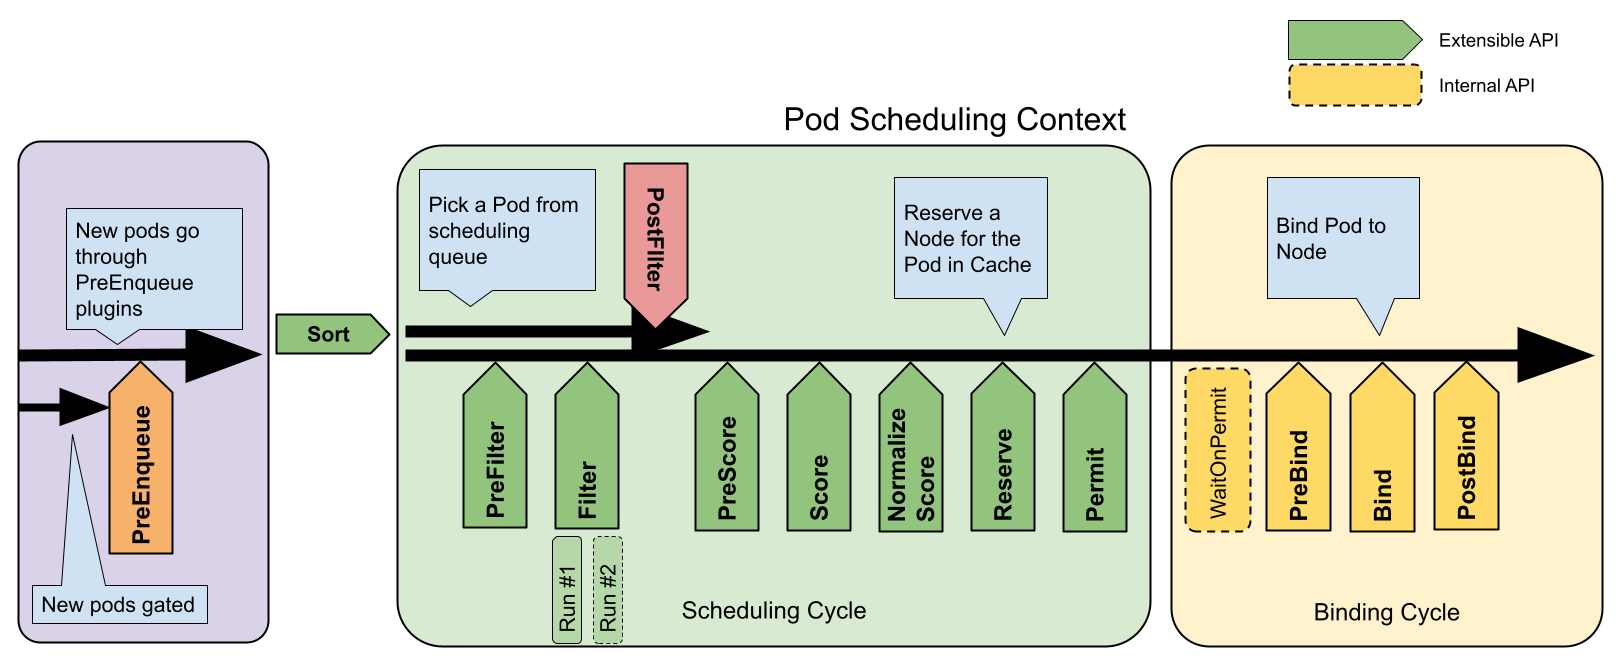
\includegraphics[width=\textwidth]{images/scheduling-framework-extensions.png}
    \caption{The available scheduling framework extension points
    \cite{scheduling-framework}.}
    \label{fig:kube-sched-framework}
\end{figure}
The scheduling framework (depicted in Figure \ref{fig:kube-sched-framework}) is
a pluggable architecture for the Kubernetes scheduler. It defines extension
points at which scheduler plugins register to be invoked. A scheduler plugin can
register to multiple extension points, with each extension point defining an
interface: a set of functions the scheduler plugin has to implement.

Developing a \textsc{Carico}-based scheduler plugin, rather than a standalone
scheduelr, simplified implemention and offered many performance benefits. First,
\textsc{Carico}'s scheduling operations (Section \ref{sec:spazio-cost-capacity}
map well to the framework's extension points. Second, the framework provides
access to efficient, pre-existing data structures and algorithms. Finally,
plugins allow customisation through selective enabling/disabling of default
plugins and ordering of custom ones. This means that the \textsc{Carico} plugin
could be used in tandem with other plugins to improve scheduling decisions.

The \textsc{Carico} scheduler tracks Pod reservations using a \verb|map| (Pod ID
to Node ID) and a Kubernetes API Pod Event Listener. During the Reserve phase, the scheduler
increments the target Node's reserve count and records Pod-Node assignment. When
the API listener detects a Pod transitioning from the 'Pending'
status, if the Pod is in its reservation \verb|map|, the scheduler decrements
the corresponding Node's reserved count.


\chapter{Evaluation}

This section is focused on the empirical evaluation of \textsc{Carico} as a Kubernetes
scheduler. As I was unable to find any telemetric-only schedulers, I decided to
compare \textsc{Carico} against the default Kubernetes scheduler throughout this section.
\texttt{kube-scheduler} is an industry-standard scheduler that was built upon
the lessons learnt from Borg \cite{}, and thus, has been thoroughly optimised
and battle tested. As \texttt{kube-scheduler} is a Pod description-based
scheduler, I use mutliple different resource requests to highlight how the
performance achieved can vary depending on description.

The chapter is divided into the following sections:
\textbf{Overhead - Section \ref{sec:eval-overhead}:} I measure the computational overhead
incurred from running the \textsc{Carico} Pods on every Node. To ascertain this effect, I
complare the Job Completion time with and without the deployment of the \textsc{Carico}
Pod DaemonSet

\textbf{Different Workloads - Sections
\ref{sec:eval-cpu-centric},\ref{sec:eval-mem-centric}, \ref{sec:eval-mixed}:}
These sections investigate the performance of \textsc{Carico} when deploying different
workloads. For each workload, I investigate four metrics: Job Completion, Number
of Running Pods, Pod Completion and Resource Usage. Job Completion measures the
time it takes for all the Pods specified by a Job to complete. This then acts as
a strong indicator of overall throughput of a scheduler. The Number of Running
Pods will be used to explain the achieved Job Completion. Pod Completion instead
focuses on the distribution of the time it takes for the Pods to complete. The
distribution gives an indication of the amount of contention that occurs during
the deployment of the Job. A tail-heavy distribution indicates high levels of
contention and that the scheduler is overloading a Node. Finally, resource
utilisation will focus on CPU and Memory utilisation. I decided to only measure
these two resources as they are the only two that are currently considered in
the scheduling decisions made by both \textsc{Carico} and the default Kubernetes
scheduler.

\textbf{Workload Isolation - Section \ref{sec:workload-isolation}:} In this
section I investigate the workload-isolation provided by \textsc{Carico} and the default
Kubernetes scheduler. Workload isoolation is considered a core component of QoS
scheduling, and thus is a useful metric to observe.

\section{Evaluation Setup}
These experiments ran on a Kubernetes cluster containing 20 virtual machines
(VMs) running on the Xen hypervisor. One of the machines is used as the master
Node, and the rest are worker Nodes. The master Node contains all the Pods in
the control plane, and during the evaluation of \textsc{Carico}, it contains the \textsc{Carico}
Scheduler and Aggregation Server. Each VM features four Intel Xeon Gold 6142
CPUs \@ 2.60Ghz with 8 GB of RAM running Ubuntu 24.04.2 LTS. Each CPU has a
single core with hyperthreading disabled. When running \texttt{kubectl describe
nodes}, each Node advertises $4000$ milli-CPU seconds and 8GB of RAM.

During the evaluation, I use a Prometheus deployment \cite{} to collect various
statistics, such as running Pod count, resource utilisation and Kubernetes
object completions.

\section{\textsc{Carico} Overhead}
\label{sec:eval-overhead}
To measure the overhead incurred from running the \textsc{Carico} pods on the Nodes, I
compared the completion time of Jobs when running on Nodes with and without the
\textsc{Carico} deployment. I considered easuring resource utilisation on a Node with
just the \textsc{Carico} Pod running, but much of the behaviour of the
\textsc{Carico} Pod occurs during container events. As a result, the measured overhead
would not represent the entire impact of the \textsc{Carico} Pod. Instead, by measuring
the overhead over Jobs, we aggregate the impact of \textsc{Carico} across multiple
container events, providing a more holistic view of its impact.

\begin{table}[H]
\centering
    \begin{tabular}{|c|c|}
    \hline
    \textbf{Number of Pods} & \textbf{\% Overhead with \textsc{Carico}} \\
    \hline
        100 & -2.33 $\pm$ 3.29 \\
        250 & -1.19 $\pm$ 2.44 \\
        500 & 4.84  $\pm$ 1.25 \\
        750 & 1.69  $\pm$ 0.42 \\
        1000 & 2.27  $\pm$ 0.66 \\
    \hline
    \end{tabular}
    \label{tab:overhead}
    \caption{The overhead incurred when running \textsc{Carico} Pods on Nodes during the
    executing of Jobs with varying Pod counts. Each Pod executed
    \texttt{bpi(2000)} and requested 200 milliseconds of CPU time.}
\end{table}

To measure \textsc{Carico}'s overhead, I used Pod's executing \texttt{bpi(2000)}. Table
\ref{tab:overhead} presents the relative change in Job Completion time with
\textsc{Carico} Pods running on the Nodes. We can see that the Job Completion time of
smaller Jobs are more noisy, therefore, resulting in an observed decrease in Job
Completion times. However, with larger and more stable Jobs, the overhead from
\textsc{Carico} is more visible. From these observations we can conclude that \textsc{Carico} has
$\approx$ 2\% overhead.
%
% For any practical projects, you should almost certainly have some kind
% of evaluation, and it's often useful to separate this out into its own
% chapter.
\section{CPU-centric Workloads}
\label{sec:eval-cpu-centric}
For this experiment, I used a CPU-heavy workload: Pods calculatig $\pi$ to 2000
digits (\texttt{bpi(2000)}). This simple workload helps visualise the impact of
combining CPU Pressure with CPU Utilisation.

\subsection{Throughput}
During the measurements with the default Kubernetes scheduler, I used the
following CPU requests: 100m, 200m, 500m, 1000m. The results are given in Table
\ref{tab:pi-2000-throughput}

\begin{table}[H]
\centering
    \begin{tabular}{|l|r|c|c|c|c|c|}
    \hline
    \textbf{Scheduler} & \textbf{Requested} & \multicolumn{5}{c|}{\textbf{Job Completion (s)}} \\
    \cline{2-7}
    &  \textbf{CPU} & \textbf{100 Pods} & \textbf{250 Pods} & \textbf{500 Pods} & \textbf{750 Pods} & \textbf{1000 Pods} \\
    \hline
    Default & 100m & 15.7 $\pm$ 0.6 & 31.7 $\pm$ 2.1 & 56 $\pm$ 1.7 & 84.7 $\pm$
        0.6 & 112 $\pm$ 0.0 \\
    Default & 200m & 15.7 $\pm$ 0.7 & 30.7 $\pm$ 0.6 & 55 $\pm$ 1 & 79 $\pm$ 0.0
        & 103 $\pm$ 1 \\
    Default & 500m & 15.7 $\pm$ 1.2 & 32 $\pm$ 2.6 & 57.7 $\pm$ 0.6 & 81 $\pm$ 2
        & 104 $\pm$ 2.1 \\
    Default & 1000m & 21 $\pm$ 2.0 & 54.7 $\pm$ 0.6 & 96 $\pm$ 2.6 & 133 $\pm$
        0.6 & 175 $\pm$ 1 \\
    \textsc{Carico} &  & 20.3 $\pm$ 0.6 & 35.3 $\pm$ 0.6 & 60.3 $\pm$ 2.5 & 89 $\pm$ 2 &
        109$\pm$ 1 \\
    \hline
    \end{tabular}
    \caption{Job Completion of Job deployments with different Pod counts. Each
    Pod executed \texttt{bpi(2000)}. For the default scheduler, the requested
    resources are also given}
    \label{tab:pi-2000-throughput}
\end{table}

From Table \ref{tab:pi-2000-throughput}, we can see how much the performance of
the default scheduler varies depending on the amount of CPU time requested.
Over-estimating requests can result in the CPU being underutilised, while
under-estimating can result in too many Pods running on a Node at once. With
\textsc{Carico}, we observed only observed a 10\% reduction in Job Completion time. This
can be attributed to its use of telemetric data: CPU utilisation amd CPU
Pressure. In Section \ref{sec:issue-with-util}, I investigated these metrics and
showed how with \texttt{bpi(2000)} Pods, these metrics indicated full capacity
when running 4-8 Pods. As the capacity signal of a Node is tied to these
metrics, the Node's will never advertise more capacity than $\approx$ 8 Nodes.

TODO: POTENTIALLY MENTION HOW 1000M AND 500M CORRESPOND TO THE LIMIT OF USING
CPU UTILISATION AND CPU PRESSURE

\subsection{Pod Completions}
\begin{table}[H]
\centering
    \begin{tabular}{|l|r|c|c|c|c|c|c|c|}
    \hline
        \bfseries Scheduler & \bfseries CPU Request & \bfseries Mean & \bfseries Std. &
        \bfseries Min. & \bfseries 25\% & \bfseries Median & \bfseries 75\% & \bfseries Max. \\
    \hline
        Kubernetes & 100m & 47.43 & 14.59 & 7.00 & 39.00 & 52.00 & 57.00 & 73.00
        \\
        Kubernetes & 500m & 9.55 & 1.49 & 5.00 & 9.00 & 10.00 & 10.00 & 14.00
        \\
        \textsc{Carico} & & 7.69 & 0.99 & 5.00 & 7.00 & 8.00 & 8.00 & 11.00 \\
    \hline
    \end{tabular}
    \caption{Pod Completion of multi-resource Job deployments with different Pod
    counts. For the default scheduler, \texttt{bpi(2000)} Pods requested 100
    milliseconds of CPU and ML Pods requested 200 milliseconds CPU and 750Mi of
    memory}
    \label{tab:cpu-pod-completions}
\end{table}
I decided to further investigate the behaviour of the schedulers by measuring
the Pod Completion time given in Figure \ref{tab:cpu-pod-completions}. From this
table, we observe that the lower request default schedulers ends up with a very
tail-heavy distribution for Pod Completions. Increasing the request to 500
milliseconds, reduces the mean by $\approx$ 80\% while also reducing the skew.
However, CARICO is able to achieve the lowest Pod Completion distribution. To
help explain the reason by this result, I also measured the number of Pods
running on each Nodes during the Job execution, and present the values in Figure
\ref{fig:pi-2000-1000x-pod-running}.

\begin{figure}[H]
    \centering
    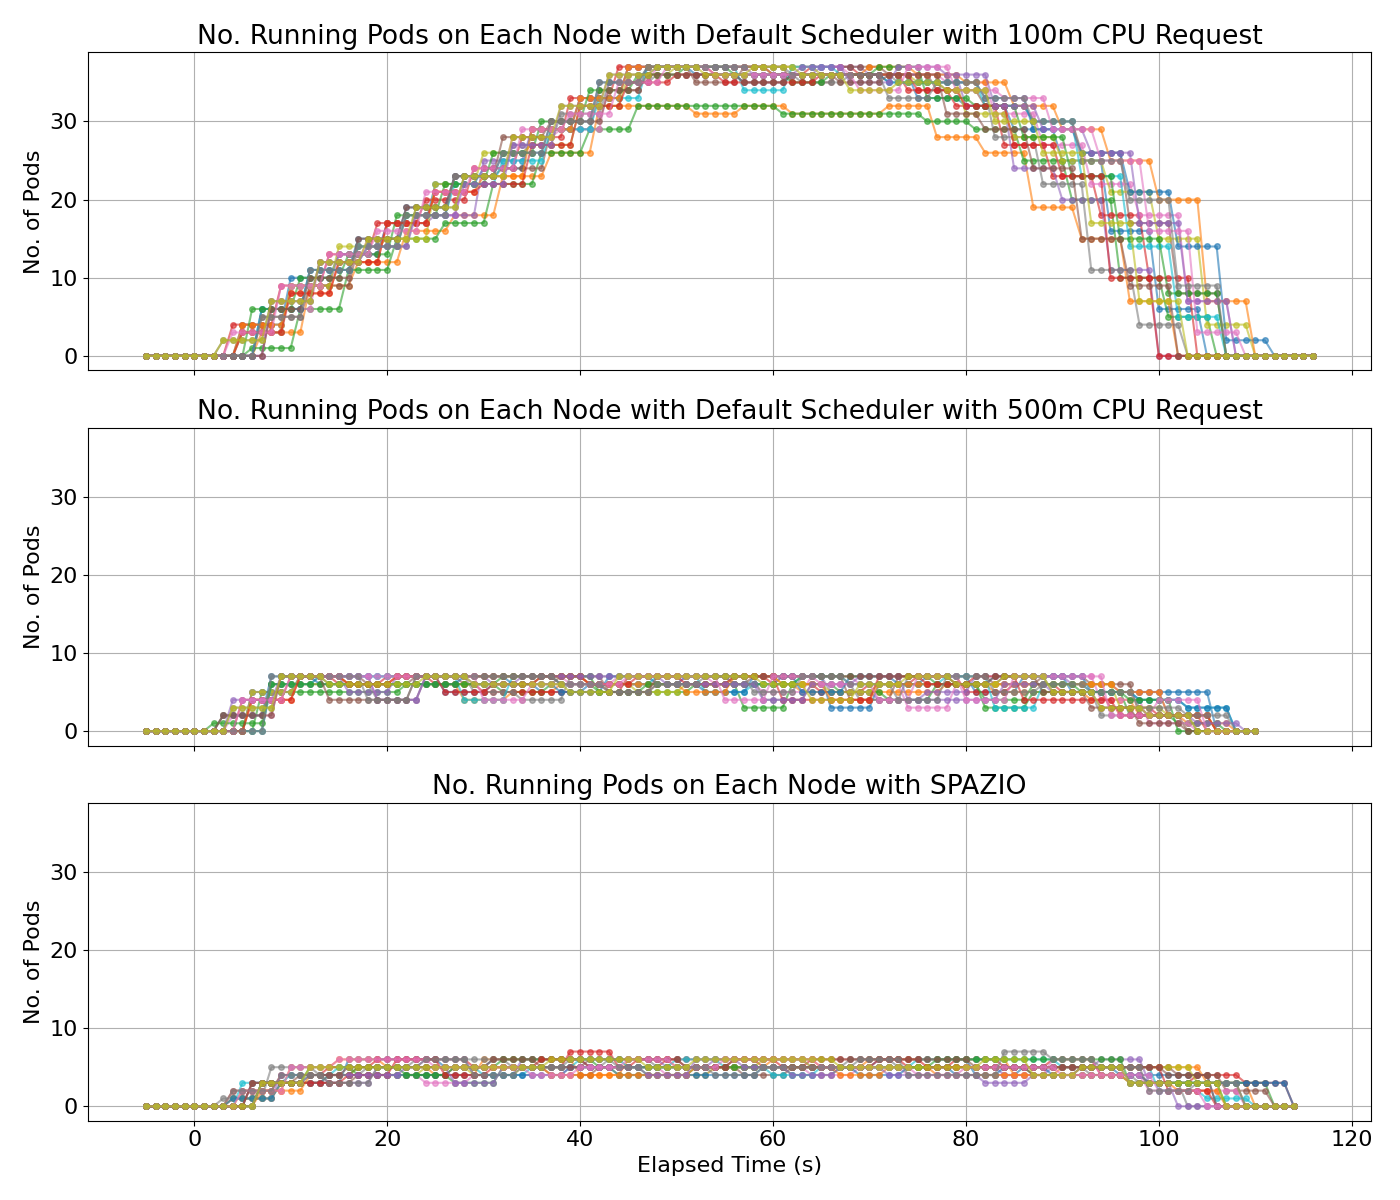
\includegraphics[width=\textwidth]{images/pi-running-pods.png}
    \caption{The number of \texttt{bpi(2000)} Pods running on a Node during the
    execution of a Job with 1000 Pods.}
    \label{fig:pi-2000-1000x-pod-running}
\end{figure}
Figure \ref{fig:pi-2000-1000x-pod-running} depicts the different approaches
taken by each scheduler. As the default Kubernetes Scheduler tackles scheduling
as if it were a bin-packing problem, it schedules as many pods that can fit on a
Node; each Node has 4000m CPU capacity, 1000m per core. As a result, the 100m
request results in a stampede of Pods while the 500m request and CARICO assign
a relatively constant number of Pods. However, the default scheduler with 500m
Pods takes the edge in terms of throughput as it achieves a higher number of
running Pods per Node.


TODO: SHOULD I TALK ABOUT NOT OVERPROVISIONING AS MEMORY USES OOM KILLS IF FULL
AND THEREFORE RISKED CORRECTNESS OF SIGNAL

\subsection{Resource Utilisation}
\begin{figure}[h]
    \centering
    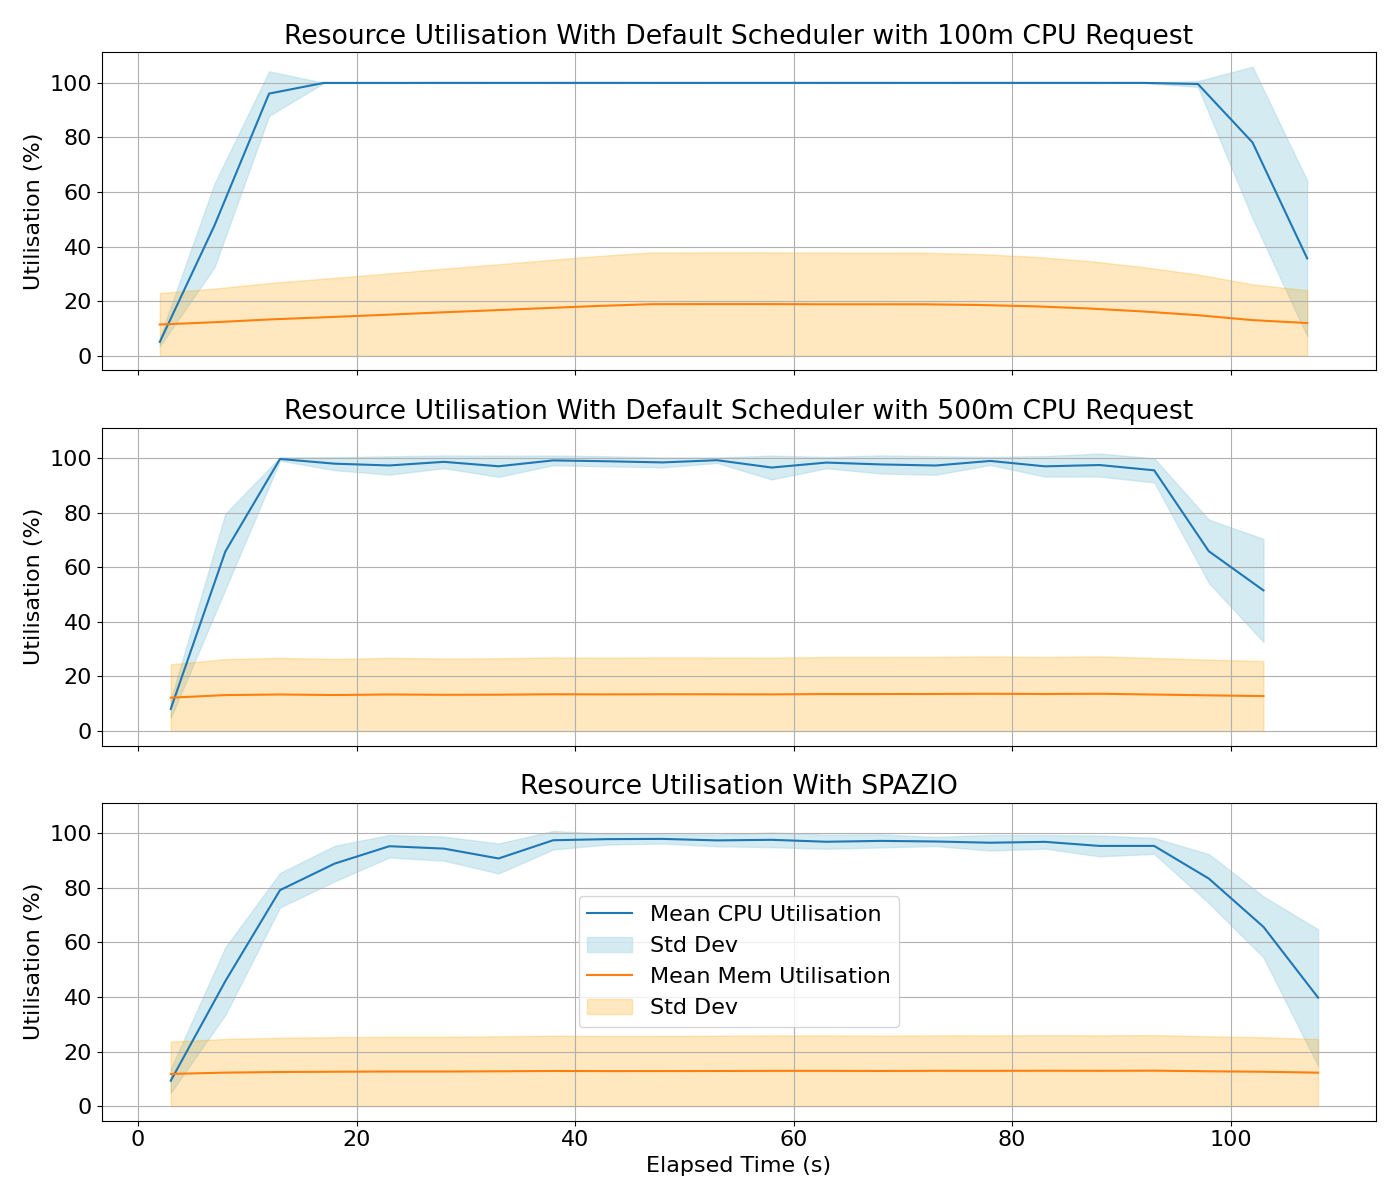
\includegraphics[width=\textwidth]{images/pi-util.png}
    \caption{the resource utilisation when scheduling a job with 1000 pods
    executing \texttt{bpi(2000)}. the top figure gives the resource utilisation
    when scheduling with the default kubernetes scheduler. the bottom figure
    gives the resource utilisation when scheduling with spazio.}
    \label{fig:pi-2000-1000x-pod-util}
\end{figure}

Figure \ref{fig:pi-2000-1000x-pod-util} shows the resource utilisation during
the execution of a Job with 1000 Pods. The default Kubernetes scheduler with
100m CPU requests achieves 100\% CPU utilisation due to the large number of Pods
running on each Node. The resulting allocation even results in a visible
increase in the Memory usage.

\section{Memory-centric Workloads}
\label{sec:eval-mem-centric}
In this experiment, I use a Job that specifies Pods that performed a small ML
workload. This workload uses a significant amount of memory, which unlike CPU,
must be carefully handled. If we increase the number of processes on a
fully-utilised CPU, it only results in each process having a smaller portion of
CPU time and degrading its performance. On the other hand, memory is less
forgiving as once memory runs out, the kernel begins OOM killing processes. This
be detrimental to Job Completion, as terminated Pods results in wasted
computations.

\subsection{Throughput}
\begin{table}[H]
\centering
    \begin{tabular}{|l|r|r|c|c|}
    \hline
    \textbf{Scheduler} & \multicolumn{2}{c|}{\textbf{Requested}} &
        \multicolumn{2}{c|}{\textbf{Job Completion (s)}} \\ \cline{2-5}
    &  \textbf{CPU} & \textbf{Memory} & \textbf{100 Pods} & \textbf{200 Pods} \\
    \hline
        Default & 200m & 750Mi & 144.3 $\pm$ 0.6 & 362 $\pm$ 20.4\\
        \textsc{Carico} &  &  & 189 $\pm$ 4.36 & 353.3 $\pm$ 12.7 \\
    \hline
    \end{tabular}
    \caption{Job Completion of Job deployments with different Pod counts. Each
    Pod executed a small ML workload. For the default scheduler, the requested
    resources are also given}
    \label{tab:ml-throughput}
\end{table}
The Job Completions from the experiment are given in Table
\ref{tab:ml-throughput}. CARICO achieves a worse performance in the smaller 100
Pod Job, but actually overtakes the default Kubernetes scheduler with the 200
Pod Job.

\subsection{Pod Completions}
\begin{table}[H]
\centering
    \begin{tabular}{|l|r|c|c|c|c|c|c|c|}
    \hline
        \bfseries Scheduler & \bfseries \# Pods & \bfseries Mean & \bfseries Std. &
        \bfseries Min. & \bfseries 25\% & \bfseries Median & \bfseries 75\% & \bfseries Max. \\
    \hline
        Kubernetes & 100 & 127.38 & 5.29 & 118 & 123.00 & 126.00 & 132.00 &
        138.00 \\
        \textsc{Carico} & 100 & 59.02 & 14.62 & 27.00 & 55.00 & 61.00 & 66.00 & 94.00 \\
        Kubernetes & 200 & 225.19 & 36.19 & 45.00 & 231.00 & 236.00 & 239.00 &
        244.00\\
        \textsc{Carico} & 200 & 64.46 & 14.33 & 23.00 & 57.75 & 67.00 & 73.25 & 89.00 \\
    \hline
    \end{tabular}
    \caption{Pod Completion of multi-resource Job deployments with different Pod
    counts. For the default scheduler, \texttt{bpi(2000)} Pods requested 100
    milliseconds of CPU and ML Pods requested 200 milliseconds CPU and 750Mi of
    memory}
    \label{tab:mem-pod-completions}
\end{table}

Table \ref{tab:mem-pod-completions} gives the Pod Completion Distribution of the
ML-based Jobs. When using the default Kubernetes scheduler, increasing the Pod
count in a Job where the resource request is underestimated, increases
drastically the average Pod Completion time as well as skewing the distribution
to become more tail-heavy. However, the distribution of Pod Completion Time
achieved by CARICO remains consistent as you increase the Job size.

\begin{figure}[H]
    \centering
    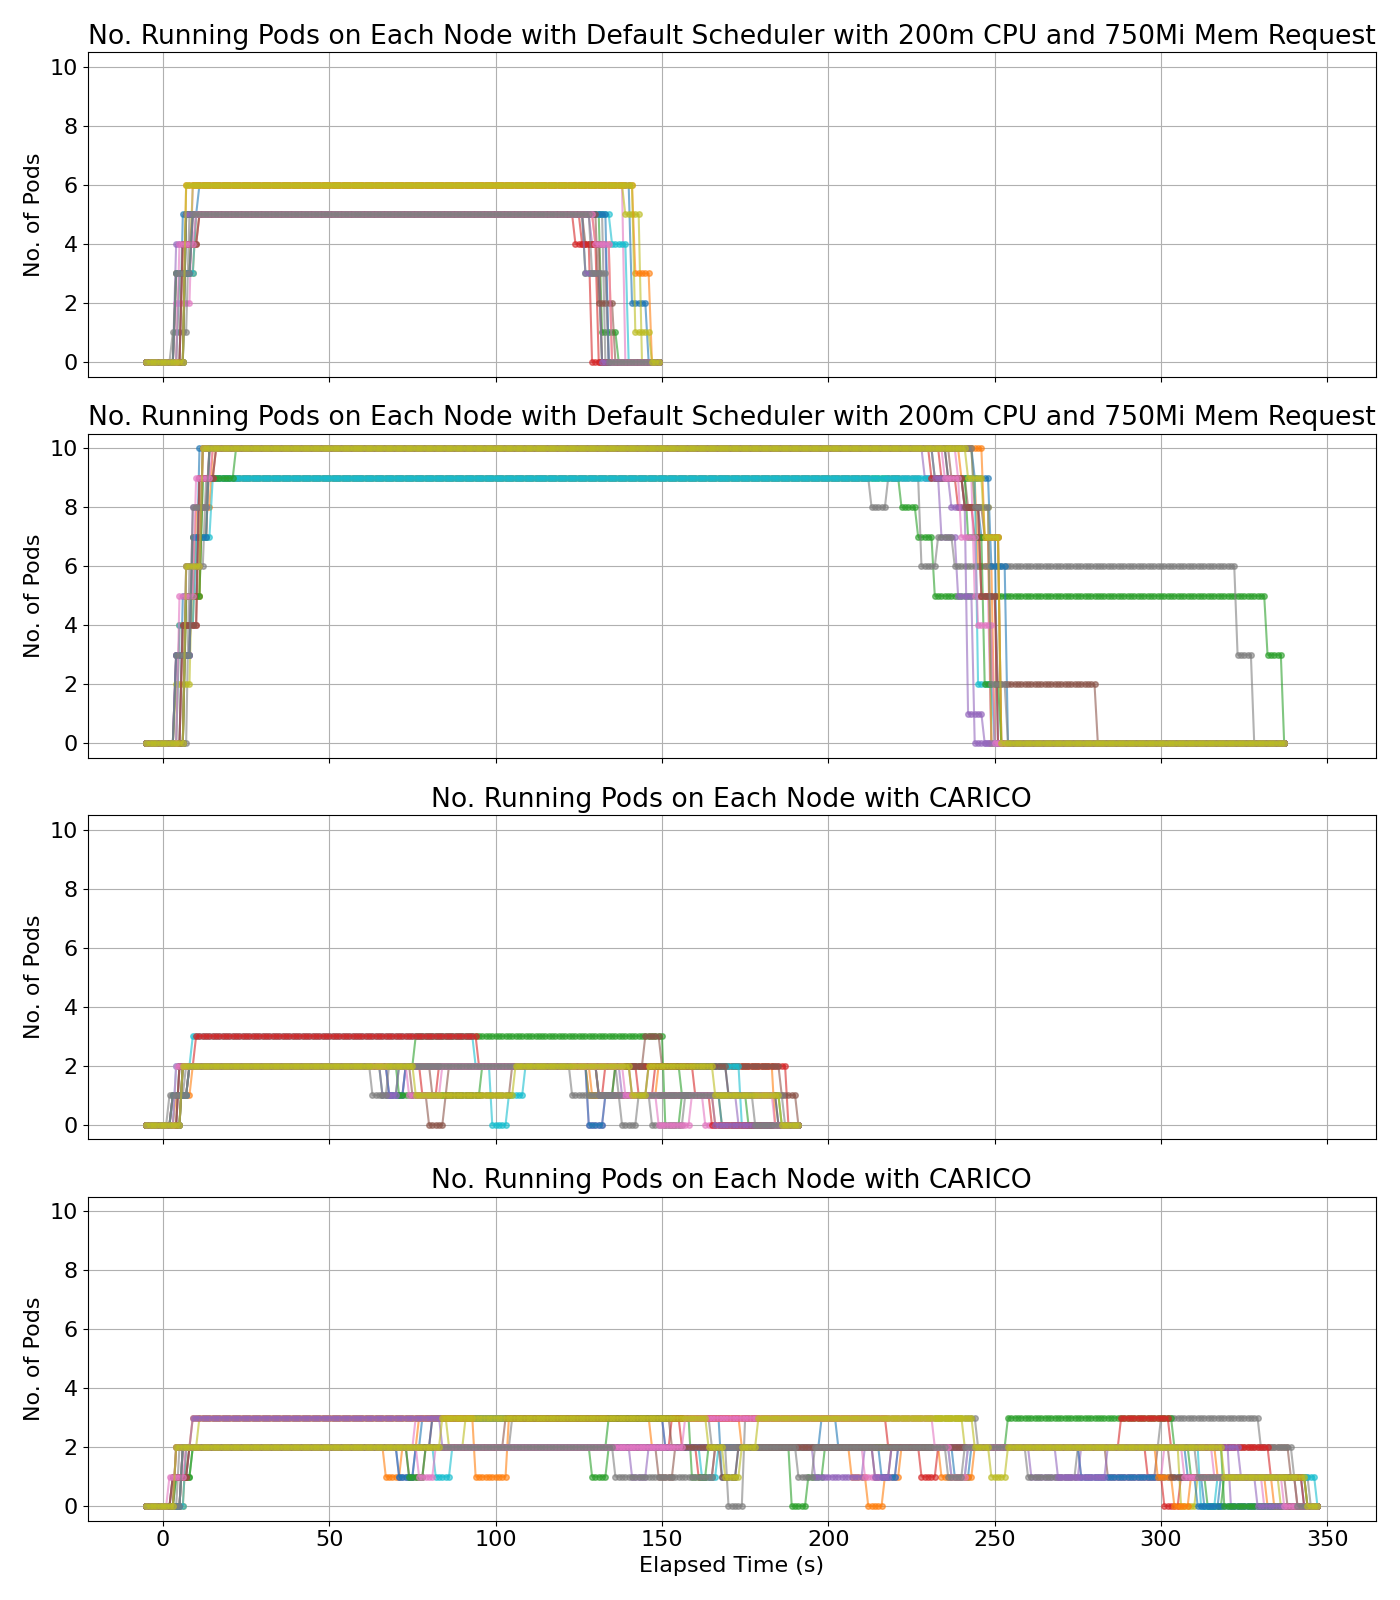
\includegraphics[width=\textwidth]{images/ml-running-pods.png}
    \caption{The number of ML Pods running on a Node during the
    execution of a Job with 100 and 200 Pods.}
    \label{fig:ml-pod-running}
\end{figure}
Figure \ref{fig:ml-pod-running} depicts the number of Pods running on each Node
at a given time. We can see how in the larger ML Job, the default scheduler is
able to allocate a majority of the Pods across the Nodes. Each Node advertises
$\approx$ 8GB of memory while each Pod requests 750MiB of Memory. All these Pods
end up competing for resources, and the overcontention increases individual
Pod completion time. The scheduler still has to wait for Pods to terminate to
free up memory. When space does become available, it is because a
stampede of Pods have terminated. While, the scheduler was able to now allocate
the remaining Pods, only a few Nodes are used while the rest become idle. This
second wave of Pods results in a slower throughput compared CARICO which ensures
1-3 Pods are always running on a Node.

\subsection{Resource Utilisation}
\begin{figure}[H]
    \centering
    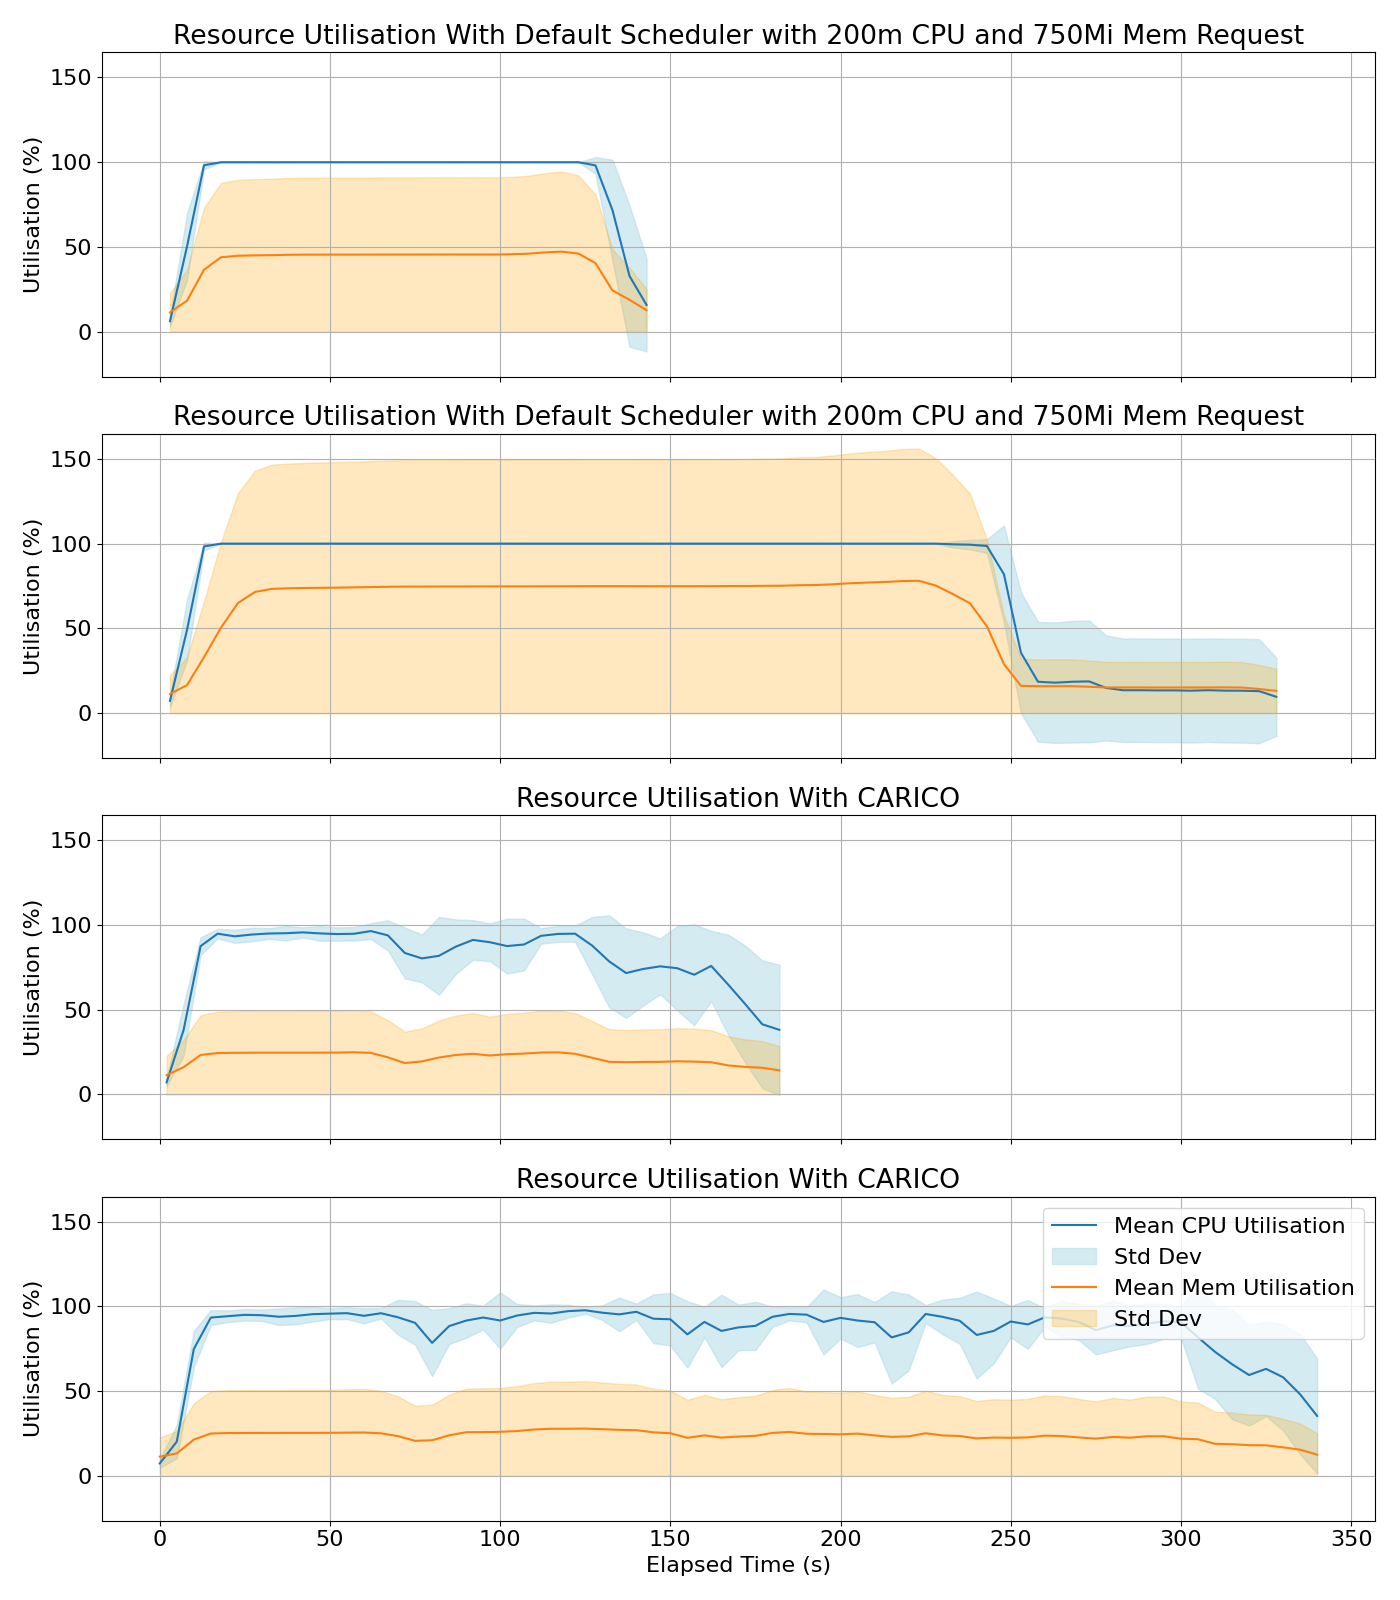
\includegraphics[width=\textwidth]{images/ml-util.png}
    \caption{The resource utilisation when scheduling a Job with 1000 Pods
    executing \texttt{bpi(2000)}. The top figure gives the resource utilisation
    when scheduling with the default Kubernetes scheduler. The bottom figure
    gives the resource utilisation when scheduling with \textsc{Carico}.}
    %\label{fig:ml-util}
\end{figure}

Figure \ref{fig:ml-pod-running} also helps to explain the resulting resource usage
depicted in Figure \ref{fig:ml-util}. While the ML workload is memory-intense,
it still contributes significantly to CPU utilisation. As the default scheduler
does not actively look at resource utilisation, it is able to allocate Pods to
Node's with fully-utilised CPUs. As a result, it achieves a higher memory usage
with both Jobs. However, we can also observe the effect of the second wave of
Pod allocations during the 200 Pod Job. During the last minute of the Job's
executing, the average CPU and Memory utilisation of the cluster have dropped to
$\approx$ 10\%; barely above their baseline utilisation.
On the other hand, CARICO is again limited by the Node's CPU metrics, achieving
a lower overall memory utilisation.

\section{Mixed Workloads}
\label{sec:eval-mixed}
In this experiment, I deployed the two Jobs defined above: a short-lived
CPU-focused workload and a longer running ML workload. This experiment evaluates
how \textsc{Carico} handles more than one type of workload.

\subsection{Throughput}
To thoroughly evaluate \textsc{Carico} in this scenario, I varied the distribution of
Pods from each Job. The observed Job Completions are given in Table
\ref{tab:mixed-throughput}.

\begin{table}[H]
\centering
    \begin{tabular}{|l|c|c|c|}
    \hline
    \textbf{Scheduler} & \multicolumn{2}{c|}{\textbf{Job Size}} &
        \textbf{Job Completion (s)} \\ \cline{2-3}
        &  \texttt{bpi(2000)} & \texttt{ML} & \\
    \hline
        Default & 500 & 20 & 105.7 $\pm$ 10.6 \\
        \textsc{Carico} & 500 & 20 & 88.7 $\pm$ 2.5 \\
        Default & 250 & 50 & 118 $\pm$ 4.58 \\
        \textsc{Carico} & 250 & 50 & 115.7 $\pm$ 0.58 \\
        Default & 100 & 100 & 149 $\pm$ 0.0 \\
        \textsc{Carico} & 100 & 100 & 192 $\pm$ 4.0 \\
    \hline
    \end{tabular}
    \caption{Job Completion of multi-resource Job deployments with different Pod
    counts. For the default scheduler, \texttt{bpi(2000)} Pods requested 100
    milliseconds of CPU and ML Pods requested 200 milliseconds CPU and 750Mi of
    memory}
    \label{tab:mixed-throughput}
\end{table}
The Job Completions from the experiment are given in Table
\ref{tab:mixed-throughput}. CARICO achieves a higher throughput during the
500-20 and 250-50 combined workloads. However, the final 100-100, we see how the
limiting throughput is now governed by the throughput achieved with the
memory-centric workload.

\subsection{Pod Completions}
Due to \textsc{Carico}'s lackluster throughput, I decided to investigate distribution of
Pods across Nodes and how it impacted Pod Completion times.

\begin{table}[H]
\centering
    \begin{tabular}{|l|c|c|c|c|c|c|c|c|}
    \hline
        \bfseries Scheduler & \bfseries Job & \bfseries Mean & \bfseries Std. &
        \bfseries Min. & \bfseries 25\% & \bfseries Median & \bfseries 75\% & \bfseries Max. \\
    \hline
        Kubernetes & \texttt{pi-2000} & 28.78 & 7.52 & 7.00 & 27.00 & 30.00 & 33.00 & 45.00 \\
        Kubernetes & ML & 65.25 & 10.53 & 49.00 & 58.25 & 64.00 & 75.25 & 82.00 \\
        \textsc{Carico} & \texttt{pi-2000} & 7.40 & 1.14 & 5.00 & 7.00 & 7.00 & 8.00 & 11.0 \\
        \textsc{Carico} & ML & 34.50 & 7.39 & 22.00 & 27.50 & 36.00 & 40.25 & 44.00 \\
    \hline
    \end{tabular}
    \caption{Pod Completion of multi-resource Job deployments with different Pod
    counts. For the default scheduler, \texttt{bpi(2000)} Pods requested 100
    milliseconds of CPU and ML Pods requested 200 milliseconds CPU and 750Mi of
    memory}
    \label{tab:mixed-pod-completions}
\end{table}

Table \ref{tab:mixed-pod-completions} gives the Pod Completion Distribution
during an execution of the 500-20 Job combination. We can observe that the
Pod Completion times for both Jobs is significantly higher with the default
scheduler compared to CARICO. This shows how CARICO is still able to achieve a
low-tailed Pod Completion time when scheduling workloads with different resource
requests.

TODO: SHOULD I ONLY INVESTIGATE WORKLOADS WE HAVE SEEN BEFORE SO THAT I CAN
COMPARE THE CHANGE IN DISTRIBUTION

\begin{figure}[H]
    \centering
    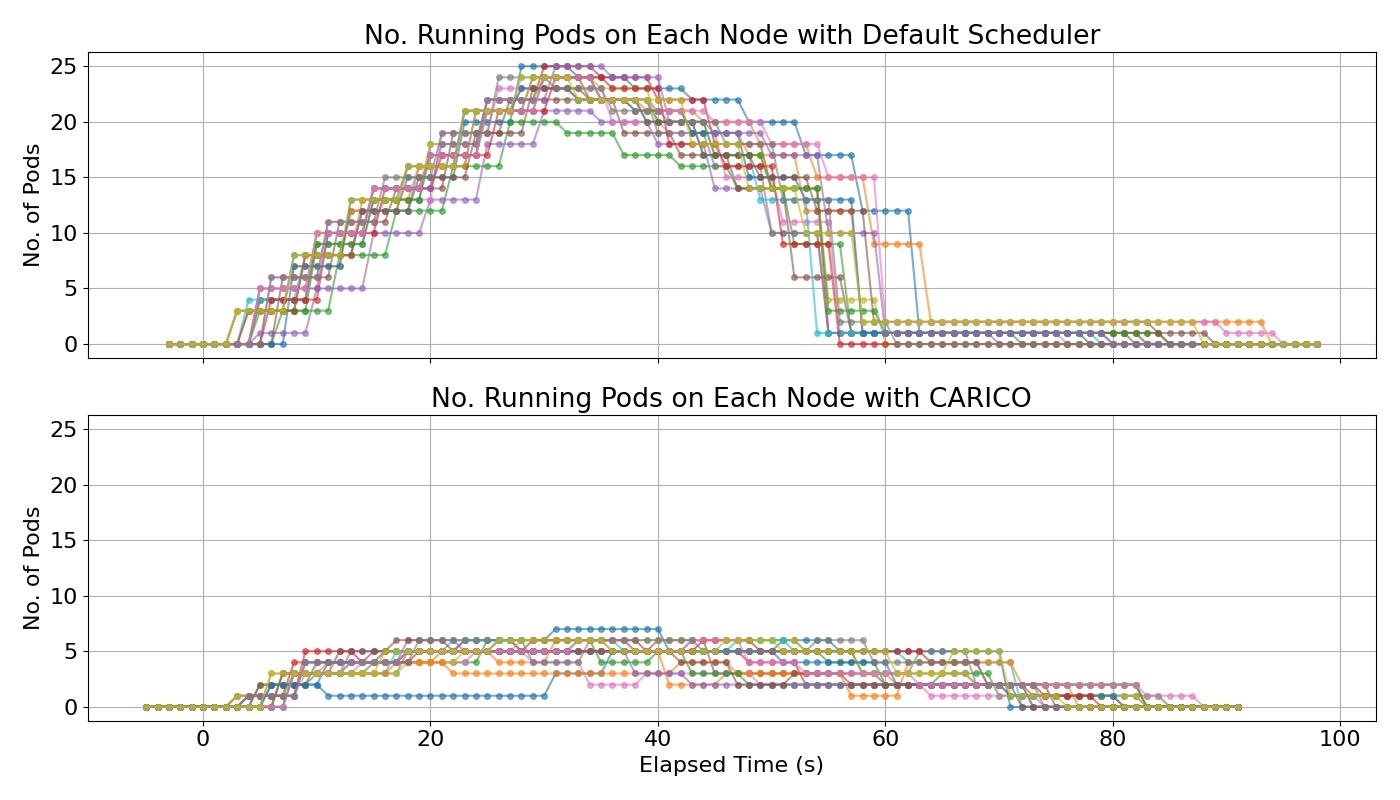
\includegraphics[width=\textwidth]{images/mixed-running-pods.png}
    \caption{The number of Pods running on a Node during the
    500-20 Job combination.}
    \label{fig:mixed-pod-running}
\end{figure}

Figure \ref{fig:mixed-pod-running} depicts the number of Pods running on each Node
at a given time. Like in \ref{fig:ml-pod-running}, the default scheduler ends up
with long-running Pods on small percentage of the Nodes in the cluster. The
default scheduler see that the Node's have enough advertised capacity, and
therefore, allocate all the Pods as they arrive. This again results in a
stampede of completions, and only a few Nodes continue to do work. However,
CARICO's rate of Pod allocation remains consistent, ensuring that Nodes have a
close to constant number of Pods.

\subsection{Resource Utilisation}

\begin{figure}[H]
    \centering
    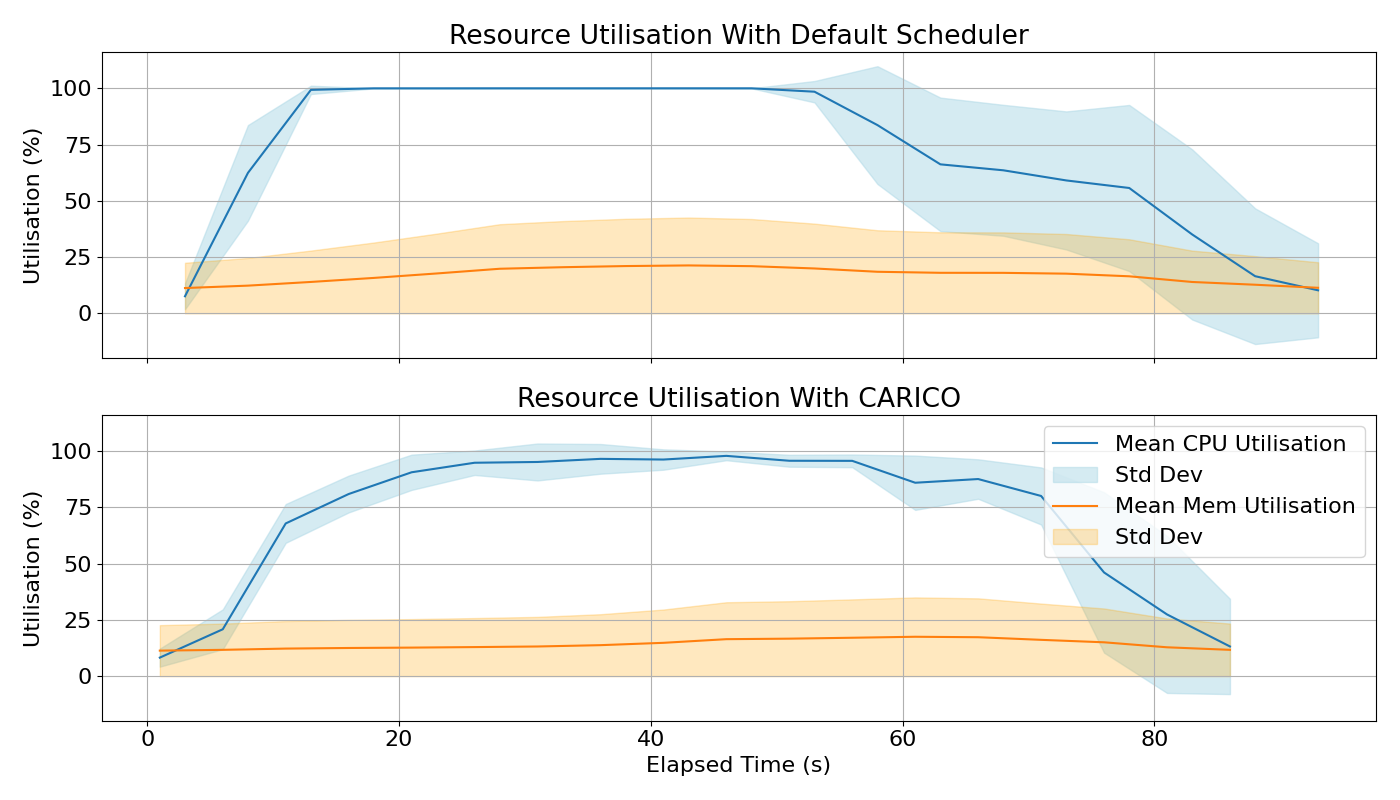
\includegraphics[width=\textwidth]{images/mixed-util.png}
    \caption{The resource utilisation when scheduling a Job with 1000 Pods
    executing \texttt{bpi(2000)}. The top figure gives the resource utilisation
    when scheduling with the default Kubernetes scheduler. The bottom figure
    gives the resource utilisation when scheduling with \textsc{Carico}.}
    \label{fig:mixed-util}
\end{figure}

Figure \ref{fig:mixed-util} shows the resource utilisation running the 500-20
combined Jobs. For the same reasons as with the  ML workload, the default
scheduler ends up with a low resource utilisation for the
latter portion of the Job exeuction. Instead, CARICO achieves a more consistent
resource utilisations, experiencing less of a fall in CPU utilisation near the
end of the Job. In this scenario, CARICO achieves a more efficient allocation of
resources.

\section{Workload Isolation}
\label{sec:workload-isolation}
To evaluate \textsc{Carico}'s QoS, I investigated how its scheduling decisions impact the
performance of already running Pods. For this experiment, I had a Pod running on
a worker Node, while another Pod periodically sent HTTP GET requests. This
polling Pod would then measure latency of the response. I then scheduled a Job
of 1000 Pods executing \texttt{bpi(2000)} across the cluster and measured how
the response latency changed. In the default schedulers case, each Pod requested
100 milliseconds of CPU time.

\begin{table}[h!]
\centering
    \begin{tabular}{|l|c|c|c|c|c|c|}
    \hline
    \textbf{Scenario} & \multicolumn{6}{c|}{\textbf{Response Latency (ms)}} \\
    \cline{2-7}
    & \textbf{Min} & \textbf{Med} & \textbf{P90} & \textbf{P95} & \textbf{P99} & \textbf{Max} \\
    \hline
    Baseline & 0.99 & 3.04 & 3.78 & 4.00 & 4.47 & 8.32 \\
    Default Scheduler & 1.07 & 10.06 & 18.61 & 22.28 & 28.82 & 54.49\\
    \textsc{Carico}  & 1.00 & 2.48 & 6.09 & 7.82 & 10.53 & 17.39\\
    \hline
    \end{tabular}
    \caption{The distribution of a servers response latency when different
    schedulers attempt to allocate a 1000 Pod Job across the server.}
    \label{tab:impacted-latency}
\end{table}

Table \ref{tab:impacted-latency} contains the measured distribution of the
response latency from the server. It shows how scheduling with the default
scheduler using 100m CPU requests, resulting a significant shift in latency
distribution. The median more than doubles and the distribution greatly shifted
towards the tail: the maximum latency was $\approx \times7$ larger. On the other
hand, when scheduling with CARICO, the median latency actually decreased.
Furthermore, while the tail distribution did increase, the max latency was only
$\approx \times2$ bigger.

\section{Limitation}
\begin{tcolorbox}[boxsep=0mm,left=2.5mm,right=2.5mm]
    \textbf{Limitations:} {\em In this section, I will go over the limitations
    of the system. I will highlight how certain metrics like CPU-Utilisations
    don't give any more information once saturated. I will also have to mention
    how due to the sub-linear pod completion time, the Kubernetes scheduler is
    able to achieve higher job throughput by packing more pods into nodes.
    }
\end{tcolorbox}

\section{Summary}
\begin{tcolorbox}[boxsep=0mm,left=2.5mm,right=2.5mm]
    \textbf{Summary:} {\em In this section, I will summarise the results of my
    evaluation section, highlighting key findings and reasoning.
    }
\end{tcolorbox}



\chapter{Conclusion and Future Work}

% As you might imagine: summarizes the dissertation, and draws any
% conclusions. Depending on the length of your work, and how well you
% write, you may not need a summary here.
%
% You will generally want to draw some conclusions, and point to
% potential future work.
%

\section{Summary}
The goal of this dissertation was to implement a telemetric-only Kubernetes
scheduler using the theory behind PRONTO as a spring-board. I based the design
of the scheduler behind PRONTO because of its federated nature and its use of
contention-based metrics.


This dissertation resembles little to what was in the Project Proposal, and I
feel this tells a lot about this project. A telemetric-only Kubernetes scheduler
was a novel and inetresting
presented an interesting and novel


\section{Future Work}


\label{lastcontentpage} % end page count here

\bibliographystyle{unsrturl}
\bibliography{report}

\appendix
\chapter{Required Lemmas for Model Interpretation}

\section{Proof: The First Left Singular Vector of Non-Negative Matrices as a
Pseudo Weighted Average}
\label{app:vector-to-avg}
Let $\mathbf{A}$ be an $m \times n$ matrix with non-negative elements $0 \leq
a_{ij} \leq 1$. Let $u_1$ be the first left singular vector and $\sigma_1$ the
corresponding singular value of $\mathbf{A}$.

\subsection{Fundamental Representation of $u_1$}
The vector $u_1$ is an eigenvector of $\mathbf{AA}^T$ associated with the
largest eigenvalue $\sigma_1^2$: $\mathbf{AA}^T = \sigma_1^2 u_1$. Let $a_j$
denote the $j$-th column of $\mathbf{A}$. Then $\mathbf{AA}^T = \sum_{j=1}^n a_j
a_j^T$. Substituting this into the eigenvalue equation and assuming $\sigma_1
\neq 0$: $\big( \sum_{j = 1}^n a_j a_j^T\big) u_1 = \sigma_1^2 u_1 \implies
\sum_{j=1}^n a_j (a_j^T u_1) = \sigma_1^2 u_1$. Thus $u_1$ can be expressed as a
linear combination of the columns of $\mathbf{A}$:
\[ u_1 = \sum_{j=1}^n \bigg(\frac{a_j^T u_1}{\sigma_1^2}\bigg) a_j =
\sum_{j=1}^n w_j a_j, \text{  where } w_j = \frac{a_j^T u_1}{\sigma_1^2} \]

\subsection{Contribution of Columns to $u_1$}
The magnitude of each weight $w_j$ is given by:
\[ |w_j| = \frac{|a_j^T u_1|}{\sigma_1^2} = \frac{\parallel a_j\parallel
|\cos(\theta_j)|}{\sigma_1^2}\]
where $\theta_j$ is the angle between column $a_j$ and $u_1$. Columns $a_j$ with
larger norms $\parallel a_j \parallel$ or those more parallel to $u_1$ (i.e.
$|\cos(\theta_j)| \approx 1$) will have weights $w_j$ of greater magnitude.
Consequently, these "larger" or more aligned columns contribute more
significantly to the sum defining $u_1$ and thus to its direction

\subsection{Non-Uniqueness of $u_1$ and Relation to Perron-Frobenius Theorem}
The singular vectors in SVD are not unique: if $\mathbf{A} =
\mathbf{U}_1\Sigma\mathbf{V}_1^T = \mathbf{U}_2\Sigma\mathbf{V}_2^T$ then
$\Sigma_1 = \Sigma_2$ but $\mathbf{U}_1 = \mathbf{U}_2\mathbf{B}_a$ and
$\mathbf{V}_1 = \mathbf{V}_2\mathbf{B}_b$ for some block diagonal unitary
matrices $\mathbf{B}_a, \mathbf{B}_b$~\cite{eftekhari2019moses}.

Since $\mathbf{A}$ has non-negative entries ($a_{ij} \geq 0$), $\mathbf{AA}^T$
is a non-negative matrix. By the Perron-Frobenius theorem, there exists an
eigenvector $u_1^+$ corresponding to the eigenvalue $\sigma_1^2$ whose
components $u_{1i}^+$ are all non-negative ($u_{1i}^+ \geq 0$). The first left
singular vector $u_1$ obtained from SVD must then be $u_1 = bu_1^+$ where $b =
\pm 1$

\subsection{Interpretation as a Pseudo Weighted Average}
\begin{itemize}
    \item \textbf{Case 1:} $b = 1 \implies u_1 = u_1^+$.\\
    In this case, $a_j^Tu_1 = a_j^Tu_1^+ = \sum_i a_{ij}u_{1i}^+ \geq 0$ (as
    $a_{ij} \geq 0, u_{1i}^+ \geq 0$).\\
    The weights $w_j = (a_j^Tu_1)/\sigma_1^2$ are therefore non-negative ($w_j
    \geq 0$).\\
    $u_1 = \sum w_ja_j$ becomes a conic combination of the non-negative column
    vectors $a_j$. This $u_1$ (itself non-negative) acts as a pseudo weighted
    average, representing a principal direction within the cone spanned by the
    $a_j$. Columns contributing larger non-negative $w_j$ pull $u_1$ more
    strongly in their direction.
    \item \textbf{Case 2:} $b = -1 \implies u_1 = -u_1^+$.\\
    Here, $a_j^Tu_1 = a_j^T(-u_1^+) =  - a_j^T(u_1^+) \leq 0$.\\
    The weights $w_j = (a_j^Tu_1)/\sigma_1^2$ are non-positive ($w_j \leq 0$).\\
    While $u_1 = \sum w_ja_j$ now involves non-positive weights for non-negative
    vectors $a_j$, the magnitudes $|w_j| = (a_j^Tu_1)/\sigma_1^2$ remain the
    same as in Case 1. Thus, columns $a_j$ that are ``larger" or more aligned
    with $u_1^+$ still contribute with greater magnitude to the sum, determining
    the orientation of the line spanned by u.
\end{itemize}

\subsection{Conclusion}
The vector $u_1$ is a linear combination of the columns of $\mathbf{A}$, $u_1 =
\sum w_j a_j$. The magnitude of the coefficient $w_j$ for each column $a_j$ is
proportional to the projection of $a_j$ onto $u_1$ (scaled by $1/\sigma_1^2$).
This means the columns with larger norms or those more aligned with the
principal direction (the line spanned by $u_1$) contribute more significantly to
defining this direction.

Irrespective of the sign $b$ (determined by the SVD algorithm), the line along
which $u_1$ lies is shaped by this weighted aggregation.

\section{Proof: Monotonicity of the First Singular Value for Non-Negative Matrices}
\label{sec:app-monotonicity}
Let $\mathbf{A}$ and $\mathbf{B}$ be $m \times n$ matrices with real entries
such that $0 \leq a_{ij} \leq b_{ij} \leq 1$ for all $i,j$. We want to show that
$\sigma_1(\mathbf{A}) \leq \sigma_1(\mathbf{B})$, where $\sigma_1(\mathbf{M})$
denotes the first (largest) singular value of a matrix $\mathbf{M}$.

\subsection{Relating Singular Values to $\mathbf{M}^T\mathbf{M}$}
\label{sec:mono-one}
The square of the first singular value, $\sigma_1(\mathbf{M})^2$, is the largest
eigenvalue of the matrix $\mathbf{M}^T\mathbf{M}$. Since
$\mathbf{M}^T\mathbf{M}$ is a symmetric positive semi-definite matrix, its
largest eigenvalue is also its spectral radius, $\rho(\mathbf{M}^T\mathbf{M})$.
Thus, $\rho(\mathbf{A})^2 = \rho(\mathbf{A}^T\mathbf{A})$ and
$\rho(\mathbf{B})^2 = \rho(\mathbf{B}^T\mathbf{B})$.

\subsection{Comparing $\mathbf{A}^T\mathbf{A}$ and $\mathbf{B}^T\mathbf{B}$}
Let $\mathbf{M}_{\mathbf{A}} = \mathbf{A}^T\mathbf{A}$ and
$\mathbf{M}_{\mathbf{B}} = \mathbf{B}^T\mathbf{B}$. The $(j,k)$-th element of
thess matrices are:
\begin{align}
    (\mathbf{M}_{\mathbf{A}})_{jk} &= \sum_{i=1}^m a_{ij}a_{ik} \\
    (\mathbf{M}_{\mathbf{B}})_{jk} &= \sum_{i=1}^m b_{ij}b_{ik}
\end{align}

Since $0 \leq a_{ij} \leq b_{ij}$ for all $i,j$:
\begin{itemize}
    \item All $a_{ij}$ and $b_{ij}$ are non-negative
    \item Therefore, $a_{ij}a_{ik} \leq b_{ij}b_{ik}$ for all $i,j,k$. Summing
        over $i$:
        \[ \sum_{i=1}^m a_{ij}a_{ik} \leq \sum_{i=1}^m b_{ij}b_{ik} \]
        This implies $(\mathbf{M}_{\mathbf{A}})_{jk} \leq
        (\mathbf{M}_{\mathbf{B}})_{jk}$ for all $j,k$. Thus, $0 \leq
        \mathbf{M}_{\mathbf{A}} \leq \mathbf{M}_{\mathbf{B}}$ element-wise. Both
        $\mathbf{M}_{\mathbf{A}}$ and $\mathbf{M}_{\mathbf{B}}$ are matrices
        with non-negative entries.
\end{itemize}

\subsection{Monotonicity of Spectral Radius}
\label{sec:mono-three}
A standard result from Perron-Frobenius theory states that if $\mathbf{X}$ and
$\mathbf{Y}$ are non-negative matrices such that $\mathbf{X} \leq \mathbf{Y}$
element-wise ($\forall i,j. x_{ij} \leq y_{ij}$), then their spectral radii satisfy $\rho(\mathbf{X}) \leq
\rho(\mathbf{Y})$. Applying this result to $\mathbf{M}_{\mathbf{A}} =
\mathbf{A}^T\mathbf{A}$ and $\mathbf{M}_{\mathbf{B}} =
\mathbf{B}^T\mathbf{B}$:
\[ \rho(\mathbf{A}^T\mathbf{A}) \leq \rho(\mathbf{B}^T\mathbf{B}) \]

\subsection{Conclusion}
From Section \ref{sec:mono-one} and \ref{sec:mono-three}:
\[ \sigma_1(\mathbf{A})^2 \leq \sigma_1(\mathbf{B})^2 \]
Since the singular values are by definition non-negative ($\sigma_1(\mathbf{M})
\geq 0$):
\[ \sigma_1(\mathbf{A}) \leq \sigma_1(\mathbf{B}) \]
This shows that if the values of a non-negative matrix $\mathbf{A}$ are
increased (while remaining non-negative, e.g., elements between $0$ and $1$),
the first singular value of the resulting matrix $\mathbf{B}$ wil greater than
or equal to that of $\mathbf{A}$.

\section{Proof: First Singular Value Behaviour in Non-Negative Concatenated
Matrices}
\label{sec:app-concatenate}
This section proves the following statement:\\
Given two non-negative matrices $\mathbf{A} \in \mathbb{R}^{m \times n_1}$ and
$\mathbf{B} \in \mathbb{R}^{m \times n_2}$, the first singular value of the
concatenated matrix $\mathbf{C} = [\mathbf{A}, \mathbf{B}]$ is greater than or
equal to the maximum of the first singular values of $\mathbf{A}$ and
$\mathbf{B}$. That is,
\[ \sigma_1([\mathbf{A}, \mathbf{B}]) \geq \max(\sigma_1(\mathbf{A}),
\sigma_1(\mathbf{B})) \]

\subsection{Setup}
Let $\mathbf{A}$ be an $m \times n_1$ matrix and $\mathbf{B}$ be an $m \times
n_2$ matrix. The concatenated matrix $\mathbf{C} = [\mathbf{A}, \mathbf{B}]$ is
an $m \times (n_1 + n_2)$ matrix. The first singular value of any matrix
$\mathbf{M}$, denoted $\sigma_1(\mathbf{M})$, is defined as its spectral norm:
\[ \sigma_1(\mathbf{M}) = \parallel \mathbf{M} \parallel_2 = \max_{\parallel x
\parallel_2 = 1} \parallel \mathbf{M}x \parallel_2 \]
where $x$ is a unit vector.

\subsection{Relating $\sigma_1(\mathbf{C})$ to $\sigma_1(\mathbf{A})$}
\label{sec:bigger-than-A}
Let $v_{\mathbf{A}}^*$ be a unit vector in $\mathbb{R}^{n_1}$ such that
$\sigma_1(\mathbf{A}) = \parallel \mathbf{A}v_{\mathbf{A}}^* \parallel_2$. Such
a vector $v_{\mathbf{A}}^*$ is the right singular vector corresponding to
$\sigma_1(\mathbf{A})$.

Consider a vector $x_0 \in \mathbb{R}^{n_1 + n_2}$ constructs as $x_0 =
\begin{bmatrix} v_{\mathbf{A}}^* \\ 0_{n_2 \times 1} \end{bmatrix}$, where
$0_{n_2 \times 1}$ is the zero vector of dimensions $n_2$.\\
The squared norm of $x_0$ is $\parallel x_0 \parallel_2^2 = \parallel
v_{\mathbf{A}}^* \parallel_2^2 + \parallel 0_{n_2 \times 1} \parallel_2^2 = 1^2
+ 0  = 1$. Thus, $x_0$ is a unit vector.

By definitions of $\sigma_1(\mathbf{C})$:
\[ \sigma_1(\mathbf{C}) = \max_{\parallel x \parallel_2 = 1} \parallel
\mathbf{C}x \parallel_2 \]
Since $x_0$ is a specific unit vector, we have:
\[ \sigma_1(\mathbf{C}) \geq \parallel \mathbf{C}x_0 \parallel_2 \]
Computing $\mathbf{C}x_0$ gives:
\[ \mathbf{C}x_0 = [\mathbf{A}, \mathbf{B}] \begin{bmatrix} v_{\mathbf{A}}^* \\
0_{n_2 \times 1} \end{bmatrix} = \mathbf{A}v_{\mathbf{A}}^* + \mathbf{B} \dot
0_{n_2 \times 1} = \mathbf{A}v_{\mathbf{A}}^* \]
Therefore,
\[ \sigma_1(\mathbf{C}) \geq \parallel \mathbf{A}v_{\mathbf{A}}^* \parallel_2 =
\sigma_1(\mathbf{A})\]

\subsection{Relating $\sigma_1(\mathbf{C})$ to $\sigma_1(\mathbf{B})$}
\label{sec:bigger-than-B}
Similarly, let $v_{\mathbf{B}}^*$ be a unit vector in $\mathbb{R}^{n_2}$ such that
$\sigma_1(\mathbf{B}) = \parallel \mathbf{B}v_{\mathbf{B}}^* \parallel_2$. Such

Consider a vector $x_1 \in \mathbb{R}^{n_1 + n_2}$ constructs as $x_1 =
\begin{bmatrix} 0_{n_1 \times 1} \\ v_{\mathbf{B}}^* \end{bmatrix}$.\\
The squared norm of $x_1$ is $\parallel x_1 \parallel_2^2 = \parallel 0_{n_1
\times 1} \parallel_2^2 + \parallel v_{\mathbf{B}}^* \parallel_2^2 = 0 + 1^2 =
1$. Thus, $x_1$ is a unit vector.

Again, by definitions of $\sigma_1(\mathbf{C})$:
\[ \sigma_1(\mathbf{C}) \geq \parallel \mathbf{C}x_1 \parallel_2 \]
Computing $\mathbf{C}x_1$ gives:
\[ \mathbf{C}x_1 = [\mathbf{A}, \mathbf{B}] \begin{bmatrix} 0_{n_1 \times 1} \\
v_{\mathbf{B}}^* \end{bmatrix} = \mathbf{A} \dot 0_{n_1 \times 1} + \mathbf{B}
v_{\mathbf{B}}^* = \mathbf{B}v_{\mathbf{B}}^* \]
Therefore,
\[ \sigma_1(\mathbf{C}) \geq \parallel \mathbf{B}v_{\mathbf{B}}^* \parallel_2 =
\sigma_1(\mathbf{B})\]

\subsection{Conclusion}
From Sections \ref{sec:bigger-than-A} and \ref{sec:bigger-than-B}, we have shown
that $\sigma_1(\mathbf{C}) \geq \sigma_1(\mathbf{A})$ and $\sigma_1(\mathbf{C})
\geq \sigma_1(\mathbf{B})$. This implies that $\sigma_1(\mathbf{C})$ must be
greater than or equal to the maximum of these two values:
\[ \sigma_1([\mathbf{A}, \mathbf{B}]) \geq \max(\sigma_1(\mathbf{A}),
\sigma_1(\mathbf{B})) \]

\section{Damped Merging: First Singular Value Behaviour with Non-Negative
Weighted Concatenated Matrices}
\label{sec:app-scale}
This section proves the following statement:
Given two non-negative matrices $\mathbf{A} \in \mathbb{R}^{m \times n_1}$ and
$\mathbf{\mathbf{B}} \in \mathbb{R}^{m \times n_2}$ and non-negative scalar weights
$\gamma_{\mathbf{A}} = \sqrt{w_{\mathbf{A}}}$ and $\gamma_{\mathbf{\mathbf{B}}} =
\sqrt{w_{\mathbf{\mathbf{B}}}}$ such that $w_{\mathbf{A}} + w_{\mathbf{\mathbf{B}}} = 1$, the
resulting first singular value and the first left
singular vector of the concatenated matrix $\mathbf{C} = [\gamma_{\mathbf{A}}\mathbf{A},
\gamma_{\mathbf{\mathbf{B}}}\mathbf{\mathbf{B}}]$ has the following property:
\[ \min(P_{\mathbf{A}}(u_{\mathbf{C}}),P_{\mathbf{\mathbf{B}}}(u_{\mathbf{C}})) \leq \sigma_{\mathbf{C}}^2 \leq
\max(P_{\mathbf{A}}(u_{\mathbf{C}}),P_{\mathbf{\mathbf{B}}}(u_{\mathbf{C}})) \]
where $\sigma_{\mathbf{C}}$ and $u_{\mathbf{C}}$ correspond to the first singular value and first
left singular vector of $\mathbf{C}$, $P_{\mathbf{M}}(u)$ is the sum of squared scalar projections
of the columns in $\mathbf{M}$ onto $u$ (let $m_j$ be the $j$-th column of $\mathbf{M}$ $P_{\mathbf{M}}(u)
= \sum_{j=1}^n (u^T m_j)^2$).

\subsection{Expanding $\sigma_1(\mathbf{C})$}
By definition, $S_{\mathbf{C}} = \sigma_1(\mathbf{C})$ and $u_{\mathbf{C}}$ is the corresponding first
singular left vector. Thus, they satisfy the eigenvalue equation for $\mathbf{C}\mathbf{C}^T$:
\[ \mathbf{C}\mathbf{C}^Tu_{\mathbf{C}} = S_{\mathbf{C}}^2 u_{\mathbf{C}} \]
Pre-multiplying by $u_{\mathbf{C}}^T$:
\begin{align}
    u_{\mathbf{C}}^T(\mathbf{C}\mathbf{C}^T u_{\mathbf{C}}) &= u_{\mathbf{C}}^T(S_{\mathbf{C}}^2 u_{\mathbf{C}}) \\
    u_{\mathbf{C}}^T \mathbf{C}\mathbf{C}^T u_{\mathbf{C}} &= S_{\mathbf{C}}^2 (u_{\mathbf{C}}^T u_{\mathbf{C}})
\end{align}
Since $u_{\mathbf{C}}$ is a unit vector, $u_{\mathbf{C}}^T u_{\mathbf{C}} = \parallel u_{\mathbf{C}} \parallel_2^2 =
1$. So,
\[ S_{\mathbf{C}}^2 = u_{\mathbf{C}}^T \mathbf{C}\mathbf{C}^T u_{\mathbf{C}} \]
Now, lets express $\mathbf{C}\mathbf{C}^T$ in terms of $\mathbf{A}$ and $\mathbf{B}$:\\
The matrix $\mathbf{C} = [\gamma_{\mathbf{A}}\mathbf{A},\gamma_{\mathbf{B}}\mathbf{B}]$.\\
Then $\mathbf{C}^T = \begin{bmatrix} \gamma_{\mathbf{A}}\mathbf{A}^T \\ \gamma_{\mathbf{B}}\mathbf{B}^T \end{bmatrix}$.\\
So, $\mathbf{C}\mathbf{C}^T = [\gamma_{\mathbf{A}}\mathbf{A},\gamma_{\mathbf{B}}\mathbf{B}]\begin{bmatrix} \gamma_{\mathbf{A}}\mathbf{A}^T \\
\gamma_{\mathbf{B}}\mathbf{B}^T \end{bmatrix} = (\gamma_{\mathbf{A}}\mathbf{A})(\gamma_{\mathbf{A}}\mathbf{A}^T) +
(\gamma_{\mathbf{B}}\mathbf{B})(\gamma_{\mathbf{B}}\mathbf{B}^T)$
\[ \mathbf{C}\mathbf{C}^T = \gamma_{\mathbf{A}}^2\mathbf{A}\mathbf{A}^T + \gamma_{\mathbf{B}}^2\mathbf{B}\mathbf{B}^T \]
Substitute this expression for $\mathbf{C}\mathbf{C}^T$ into the equation for $S_{\mathbf{C}}^2$:
\begin{align}
    S_{\mathbf{C}}^2 &= u_{\mathbf{C}}^T (\gamma_{\mathbf{A}}^2\mathbf{A}\mathbf{A}^T + \gamma_{\mathbf{B}}^2\mathbf{B}\mathbf{B}^T)u_{\mathbf{C}} \\
    S_{\mathbf{C}}^2 &= \gamma_{\mathbf{A}}^2(u_{\mathbf{C}}^T\mathbf{A}\mathbf{A}^Tu_{\mathbf{C}}) + \gamma_{\mathbf{B}}^2(u_{\mathbf{C}}^T\mathbf{A}\mathbf{A}^Tu_{\mathbf{C}})
\end{align}
Using the definitions for $P_{\mathbf{A}}(u_{\mathbf{C}})$ and $P_{\mathbf{B}}(u_{\mathbf{C}})$:
\begin{itemize}
    \item $P_{\mathbf{A}}(u_{\mathbf{C}}) = u_{\mathbf{C}}^T\mathbf{A}\mathbf{A}^Tu_{\mathbf{C}}$ (sum of squared projections of columns of $\mathbf{A}$ onto $u_{\mathbf{C}}$
    \item $P_{\mathbf{B}}(u_{\mathbf{C}}) = u_{\mathbf{C}}^T\mathbf{B}\mathbf{B}^Tu_{\mathbf{C}}$ (sum of squared projections of columns of $\mathbf{B}$ onto $u_{\mathbf{C}}$
\end{itemize}
This means the equation becomes:
\[ S_{\mathbf{C}}^2 = \gamma_{\mathbf{A}}^2P_{\mathbf{A}}(u_{\mathbf{C}}) + \gamma_{\mathbf{B}}^2P_{\mathbf{B}}(u_{\mathbf{C}}) \]
We are given weights $\gamma_{\mathbf{A}}, \gamma_{\mathbf{B}}$ such that $\gamma_{\mathbf{A}}^2 \geq 0,
\gamma_{\mathbf{B}}^2 \geq 0$, and $\gamma_{\mathbf{A}}^2 + \gamma_{\mathbf{B}}^2 = 1$. This means that
$S_{\mathbf{C}}^2$ is a convex combination of the two values $P_{\mathbf{A}}(u_{\mathbf{C}})$ and
$P_{\mathbf{B}}(u_{\mathbf{C}})$.
A fundamental property of convex combinations is that they always lie between
the minimum and maximum of the values being combined.\\
Let $x = P_{\mathbf{A}}(u_{\mathbf{C}})$ and $y = P_{\mathbf{B}}(u_{\mathbf{C}})$. Then $S_{\mathbf{C}}^2 = \gamma_{\mathbf{A}}^2 x +
\gamma_{\mathbf{B}}^2 y$.\\
If $x \leq y$:
\begin{itemize}
    \item $\min(x,y) = x = (\gamma_{\mathbf{A}}^2 + \gamma_{\mathbf{B}}^2)x = \gamma_{\mathbf{A}}^2 x +
        \gamma_{\mathbf{B}}^2 x \leq \gamma_{\mathbf{A}}^2 x + \gamma_{\mathbf{B}}^2 y = S_{\mathbf{C}}^2$ (since
        $\gamma_{\mathbf{B}}^2 \geq 0$ and $x \leq y$).
    \item $\max(x,y) = y = (\gamma_{\mathbf{A}}^2 + \gamma_{\mathbf{B}}^2)y = \gamma_{\mathbf{A}}^2 y +
        \gamma_{\mathbf{B}}^2 y \geq \gamma_{\mathbf{A}}^2 x + \gamma_{\mathbf{B}}^2 y = S_{\mathbf{C}}^2$ (since
        $\gamma_{\mathbf{A}}^2 \geq 0$ and $x \leq y$).
\end{itemize}
A similar argument holds if $y \leq x$. Therefore:
\[ \min(P_{\mathbf{A}}(u_{\mathbf{\mathbf{C}}}),P_{\mathbf{\mathbf{B}}}(u_{\mathbf{\mathbf{C}}})) \leq \sigma_{\mathbf{\mathbf{C}}}^2 \leq
\max(P_{\mathbf{A}}(u_{\mathbf{\mathbf{C}}}),P_{\mathbf{\mathbf{B}}}(u_{\mathbf{\mathbf{C}}})) \]

\chapter{Evaluation Setup}

\section{Cluster Setup}

These experiments ran on a Kubernetes cluster containing 20 virtual machines
(VMs) running on the Xen hypervisor. One of the machines is used as the master
Node, and the rest are worker Nodes. The master Node contains all the Pods in
the control plane, and during the evaluation of \textsc{Carico}, it contains the \textsc{Carico}
Scheduler and Aggregation Server. Each VM advertises four Intel Xeon Gold 6142
CPUs \@ 2.60GHz with 8 GB of RAM running Ubuntu 24.04.2 LTS. Each CPU has a
single core with hyper-threading disabled. When running \texttt{kubectl describe
nodes}, each Node advertises $4000$ milliCPU seconds and 8GB of RAM.

During the evaluation, I use a Prometheus deployment \cite{} to collect various
statistics, such as running Pod count, resource utilisation and Kubernetes
object completions.

%
% For any practical projects, you should almost certainly have some kind
% of evaluation, and it's often useful to separate this out into its own
% chapter.

\section{Experimental Workloads}
During the experiments I used very short-lived workloads; workloads that take
less than a minute to complete. While data canters can expect to receive
longer-running workloads, using them in the evaluation was not feasible due to
the need to run experiments multiple times and limited time. Short-lived tasks
can still provide valuable insights into the performance of a scheduler as their
short completion time makes the impact of poor scheduling decisions more
significant and easier to observe.

During this evaluation, I used two types of workloads:
\begin{enumerate}
    \item \texttt{pi-2000}: A short-lived CPU-focused workload where a Pod
        computes the value of $\pi$ to 2000 decimal points.
    \item \texttt{sklearn}: A longer-running workload with a larger memory
        footprint. This Pod executes a script which uses
        \texttt{sklearn} which trains a small neural network classifier ($512$
        features, $16$ classes, $8$ hidden layers each containing $1024$
        neurons) on 5000 randomly generated samples before running inference on
        another set of 5000 randomly generated samples.
\end{enumerate}
Investigating metrics when running \texttt{pi-2000} and \texttt{sklearn} Jobs
separately demonstrates how \textsc{Carico} handles opposing resource usage
characteristics (CPU-focused vs memory-focused). Furthermore, when executing
both these Jobs concurrently, the difference in runtime helps investigate how
\textsc{Carico} also handles workloads with different running times.

% In this experiment, I use a Job that specifies Pods that performed a small ML
% workload. This workload uses a significant amount of memory, which unlike CPU,
% must be carefully handled. If we increase the number of processes on a
% fully-utilised CPU, it only results in each process having a smaller portion of
% CPU time and degrading its performance. On the other hand, memory is less
% forgiving as once memory runs out, the kernel begins OOM killing processes. This
% be detrimental to Job Completion, as terminated Pods results in wasted
% computations.
%




\label{lastpage}
\end{document}
